% !TEX TS-program = pdflatex
% !TEX encoding = UTF-8 Unicode

% This file is a template using the "beamer" package to create slides for a talk or presentation
% - Talk at a conference/colloquium.
% - Talk length is about 20min.
% - Style is ornate.

% MODIFIED by Jonathan Kew, 2008-07-06
% The header comments and encoding in this file were modified for inclusion with TeXworks.
% The content is otherwise unchanged from the original distributed with the beamer package.

\documentclass[1pt]{beamer}
\usefonttheme[onlymath]{serif}
\usepackage{media9}
% \usepackage{beamerthemeshadow}
\usepackage[slovene]{babel}
% or whatever
\setbeamercovered{transparent}
\usepackage{caption}
\captionsetup[figure]{labelformat=empty}% redefines the caption setup of the figures environment in the beamer class.
\usepackage{lmodern}
\usepackage{bm}
\usepackage{units}
\usepackage[utf8]{inputenc}
\usepackage{amsmath}
\usepackage[export]{adjustbox}
% \usepackage{fullpage}
\usepackage{mathrsfs}
\usepackage{amsfonts}
\usepackage{amssymb}
\usepackage{fancyhdr}
\usepackage{mathtools}

\newcommand{\iu}{{i\mkern1mu}}
\newcommand{\bra}[1]{\langle #1 \vert}
\newcommand{\ket}[1]{\vert#1\rangle}
\newcommand{\avg}[1]{\left\langle#1\right\rangle}
\newcommand{\norm}[1]{\left\Vert #1 \right\Vert}
\newcommand{\braket}[2]{\left\langle #1 \vert#2 \right\rangle}
\newcommand{\obraket}[3]{\left\langle #1 \vert #2 \vert #3 \right \rangle}
\usepackage{times}
% \usepackage[utf8]{fontenc}
\newcommand{\dd}{\,\mathrm{d}}
\newcommand{\ddd}{\mathrm{d}}
\newcommand{\ii}{\mathrm{i}}
\usepackage{mhchem}
\usepackage{units}
% Copyright 2004 by Till Tantau <tantau@users.sourceforge.net>.
%
% In principle, this file can be redistributed and/or modified under
% the terms of the GNU Public License, version 2.
%
% However, this file is supposed to be a template to be modified
% for your own needs. For this reason, if you use this file as a
% template and not specifically distribute it as part of a another
% package/program, I grant the extra permission to freely copy and
% modify this file as you see fit and even to delete this copyright
% notice. 
\mode<presentation>
{
\usetheme{AnnArbor}
\usecolortheme{beaver}
\setbeamertemplate{frametitle}[default][center]
\setbeamertemplate{headline}{}
}

\usepackage{bm}


\title[Spektralne lastnosti in MBL] % (optional, use only with long paper titles)
{Spektralne lastnosti modela $t$-$J$ in večdelčna lokalizacija}

%
\includegraphics[width=0.35\textwidth]{logo_fmf_uni-lj_en.pdf}\\[8ex] 

\author[Jan Šuntajs] % (optional, use only with lots of authors)
{Avtor: Jan Šuntajs \\ 
Mentor: prof. dr. Janez Bonča \\
Somentor: doc. dr. Lev Vidmar}
\centering
\titlegraphic{
\includegraphics[width=4cm]{logo_fmf_uni-lj_sl.pdf}
}

% - Give the names in the same order as the appear in the paper.
% - Use the \inst{?} command only if the authors have different
%   affiliation.

%\institute[University of Ljubljana, Faculty of Mathematics and Physics] % (optional, but mostly needed)
%{
%  \inst{1}%
%  Department of Computer Science\\
%  University of Somewhere
%  \and
%  \inst{2}%
%  Department of Theoretical Philosophy\\
%  University of Elsewhere}
% - Use the \inst command only if there are several affiliations.
% - Keep it simple, no one is interested in your street address.

%\date[CFP 2003] % (optional, should be abbreviation of conference name)
%{Conference on Fabulous Presentations, 2003}
% - Either use conference name or its abbreviation.
% - Not really informative to the audience, more for people (including
%   yourself) who are reading the slides online



% If you have a file called "university-logo-filename.xxx", where xxx
% is a graphic format that can be processed by latex or pdflatex,
% resp., then you can add a logo as follows:
%
% \pgfdeclareimage[height=0.8cm]{university-logo}{logo_fmf_uni-lj_en.pdf}
% \logo{\pgfuseimage{university-logo}}

% If you wish to uncover everything in a step-wise fashion, uncomment
% the following command: 

%\beamerdefaultoverlayspecification{<+->}


\begin{document}

\begin{frame}
  \titlepage
\end{frame}

% Structuring a talk is a difficult task and the following structure
% may not be suitable. Here are some rules that apply for this
% solution: 

% - Exactly two or three sections (other than the summary).
% - At *most* three subsections per section.
% - Talk about 30s to 2min per frame. So there should be between about
%   15 and 30 frames, all told.

% - A conference audience is likely to know very little of what you
%   are going to talk about. So *simplify*!
% - In a 20min talk, getting the main ideas across is hard
%   enough. Leave out details, even if it means being less precise than
%   you think necessary% - If you omit details that are vital to the proof/implementation,
%   just say so once. Everybody will be happy with that.

\begin{frame}{Predstavitev v štirih točkah}
\begin{enumerate}
	\only<1->{
	\onslide<2->{
	\item Nastop \textbf{večdelčne lokalizacije} (\textbf{MBL}) v modelu $t$-$J$ \vspace{10mm}}
	\onslide<3->{
	\item Vloga \textbf{spinskega} in \textbf{potencialnega} nereda \vspace{10mm}}
	\onslide<4->{
	\item Metoda: \textbf{polna numerična diagonalizacija} \vspace{10mm}}
	\onslide<5->{
	\item Indikatorji:\vspace{5mm}
		\begin{itemize}
			\item Povprečno razmerje razmikov med sosednjimi nivoji
			\item \textbf{Spektralni oblikovni faktor} (\textbf{SFF})
			\item Prepletenostna entropija \textbf{lastnih stanj}
		\end{itemize}}
		}
\end{enumerate}

\end{frame}


% \begin{frame}{Raziskave lokalizacijskih pojavov}
% Začetki segajo v leto 1958 ...
% \only<1->{\begin{figure}
% \centering{
% 
\includegraphics[width=0.9\textwidth]{and_orig_crop.pdf}}
% % \caption{}
% \end{figure}}
% \only<2->{
% ... danes - večdelčna lokalizacija (\textbf{MBL}) 
% \begin{figure}
% \centering{
% 
\includegraphics[width=0.45\textwidth]{mbl_crop.pdf}}
% \caption{Google Scholar: 789 citatov do septembra 2018}
% \end{figure}}
% \end{frame}

\begin{frame}{\textbf{MBL} - glavni poudarki}
\only<1->{
\onslide<2->{
\begin{minipage}{0.4\textwidth}
\begin{itemize}
\item \textbf{Zaprti} kvantni sistemi 
\end{itemize}
\end{minipage}\hfill
\begin{minipage}{0.55\textwidth}
\begin{figure}
\centering{
\includegraphics[trim=0 0 340 0,clip,width=0.87\textwidth]<2->{nandkishore_huse_reservoir.pdf}}
\caption{Nandkishore, Huse, 2015}
\end{figure}
\end{minipage}}\vspace{1mm}
\only<2->{	
	\onslide<3->{
	\begin{itemize}
		\item \textbf{Meddelčne interakcije}
	\end{itemize}
	}
}
\only<3->{
\onslide<4->{
\begin{minipage}{0.5\textwidth}
\begin{itemize}
\item Prisotnost \textbf{nereda} 
\end{itemize}
\end{minipage}\hfill
\begin{minipage}{0.4\textwidth}
\begin{figure}[r]

\includegraphics[trim=0 0 0 0,clip,width=0.6\textwidth, center]<4->{disorder_scheme.pdf}
% \caption{Nandkishore, Huse, 2015}
\end{figure}
\end{minipage}}}

\only<4->{	
	\onslide<5->{
	\begin{itemize}
		\item Odsotnost \textbf{TERMALIZACIJE} 
	\end{itemize}
	}
}
}
\end{frame}

\begin{frame}{Vsebina}
\begin{enumerate}
	\item Značilnosti MBL sistemov\vspace{2.5mm}
	\begin{itemize}
		\item Hipoteza termalizacije lastnih stanj (\textbf{ETH})\vspace{5mm}
	\end{itemize}
	\item Vpeljava modela $t$-$J$\vspace{5mm}

	\item Predstavitev numeričnih rezultatov\vspace{2.5mm}
	\begin{itemize}
		\item Statistika sosednjih energijskih nivojev
		\item \textbf{Spektralni oblikovni faktor} (\textbf{SFF})
		\item Prepletenostna entropija 
		\vspace{5mm}
	\end{itemize}
	\item Zaključek
\end{enumerate}
\end{frame}

\begin{frame}{Značilnosti MBL sistemov}
% \only<1->{
\onslide<2->{
\begin{minipage}{0.3\textwidth}
\begin{itemize}
\item \textbf{NEERGODIČNOST} \vspace{10mm}
\end{itemize}
\end{minipage}\hfill
\begin{minipage}{0.67\textwidth}
\begin{figure}
\centering{
\includegraphics[width=0.67\textwidth]<2->{abanin_thermalization_scheme.pdf}}
\caption{Abanin, Altman, Bloch, Serbyn, 2018}
\end{figure}
\end{minipage}}
% \only<2->{
\onslide<3->{
\begin{itemize}
% \item \textbf{NO} DC conductivity \vspace{7mm}

\item \textbf{PREPLETENOSTNA ENTROPIJA:}\vspace{0.25mm}
	\begin{itemize}
		\item \textbf{Površinsko skaliranje za lastna stanja}
		\item Logaritemsko naraščanje s časom
	\end{itemize}
\begin{figure}
\centering{
\includegraphics[width=0.6\textwidth]<3->{znid_pros_prel_excerpt.pdf}}
\end{figure}
\end{itemize}}
% \only<3->{
\onslide<4->{ 
\vspace{3mm}
\begin{itemize}
\item \textbf{POSEBNE LASTNOSTI ENERGIJSKIH SPEKTROV}	
\begin{itemize}
	\item Predmet naše numerične analize
	\end{itemize}
\end{itemize}}


\end{frame}
\begin{frame}{Hipoteza termalizacije lastnih stanj (\textbf{ETH})}
\onslide<1->{
Če sistem termalizira $\Longleftrightarrow$  \textbf{lastna stanja} $\ket{m}$ so \textbf{``TERMALNA''}\vspace{1mm}
$$\Bigg\Updownarrow$$\vspace{6mm}
Pričakovane vrednosti opazljivk so enake ansambelskim povprečjem:
$$\bra{m} \hat{O} \ket{m}=\langle \hat{O} \rangle_T$$ \\ \vspace{10mm}}
\onslide<2->{
ETH ne velja v \textbf{INTEGRABILNIH} in \textbf{MBL} sistemih}

\end{frame}

\begin{frame}{Model $t$-$J$}
\only<1>{
\begin{alertblock}{Hamiltonka}
$$H=-t\sum\limits_{i, \sigma} \left(\tilde{c}_{i,\sigma}^\dagger\tilde{c}_{i+1,\sigma} + c.c. \right) + J\sum\limits_i \pmb{S}_i\cdot\pmb{S}_{i+1} + \sum\limits_i h_iS_i^z + \sum\limits_{i,\sigma} u_i n_{i,\sigma}$$
\end{alertblock}
\begin{itemize}
 \item Projicirani fermionski operatorji: $\tilde{c}_{i,\sigma}=(1-n_{i,-\sigma})c_{i,\sigma}$ \vspace{5mm}
 \item $h_i, u_i$: spinski in vrzelni nered, škatlasti porazdelitvi s parametroma $W$ in $H$ \vspace{5mm}
 \item Preučujemo: 1D, PBC primer, $S^z=0$
\end{itemize}}
\only<2>{
\begin{figure}
\centering{
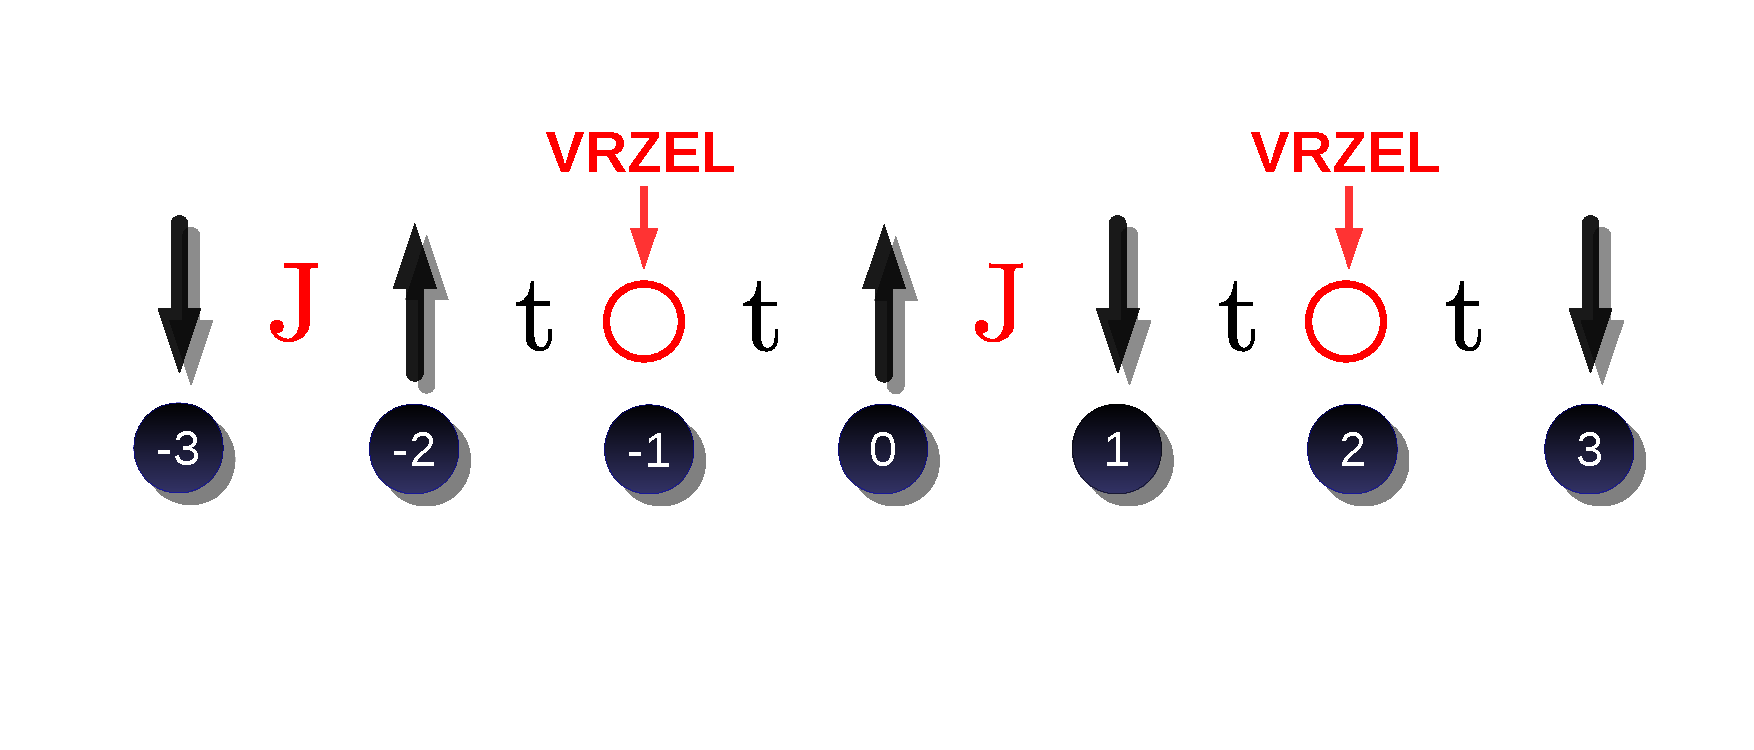
\includegraphics[width=0.5\textwidth]{tJ_scheme.pdf}}
\caption{Oznake: $L$ - št. mest, $N_h$ - št. vrzeli, $N_u$ - število spinov $\uparrow$	}
\end{figure}
\begin{figure}
\centering{
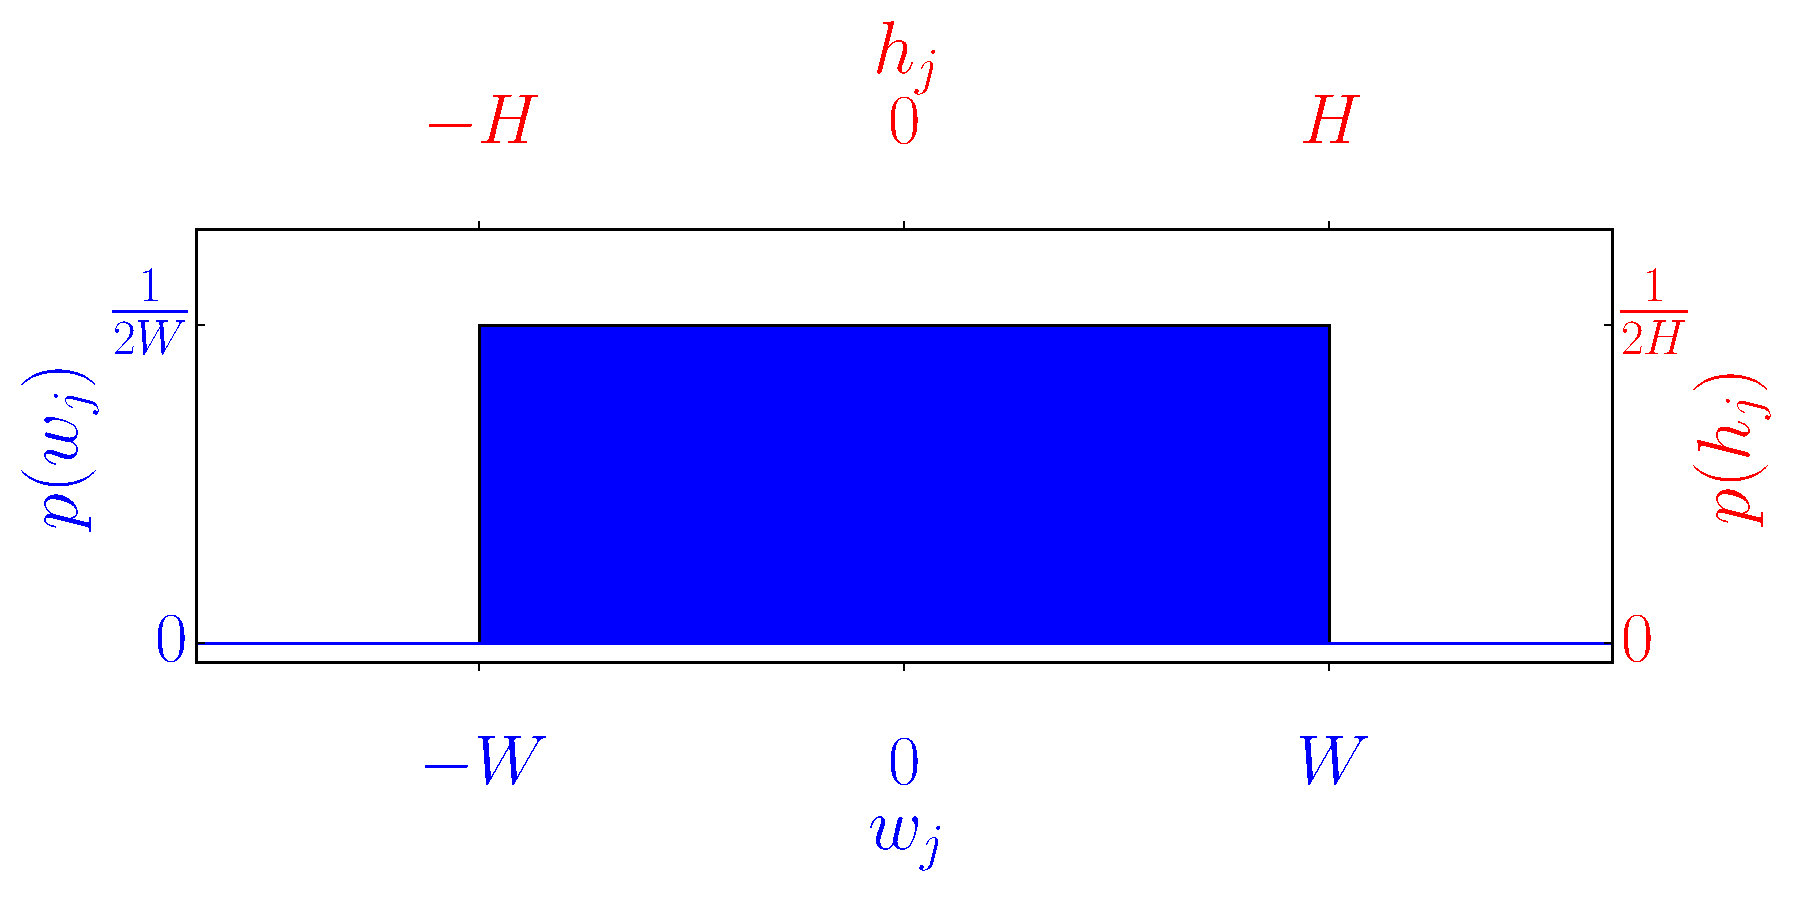
\includegraphics[width=0.5\textwidth]{prob_dist.pdf}}
\caption{Spinski ($W$) in vrzelni ($H$) nered}
\end{figure}
}
\end{frame}

\begin{frame}{Preučevanje spektralne statistike}
\only<1>{
\begin{itemize}
\item Preučujemo \textbf{porazdelitev razmikov} med sosednjimi nivoji v spektru hamiltonke \vspace{7mm}
\item Upoštevamo \textbf{teorijo naključnih matrik (RMT):} \vspace{5mm}
	\begin{itemize}
		\item \textbf{Ergodični} sistemi: spektralna statistika ustreza Gaussovemu ortogonalnemu ansamblu (\textbf{GOE}) \vspace{3mm}
		\item \textbf{MBL} sistemi: sosednji nivoji porazdeljeni v skladu s \textbf{Poissonovo} porazdelitvijo, med njimi ni odboja

	\end{itemize}\vspace{5mm}
% \item Further reading:
% 	\begin{itemize}
% 		\item Oganesyan, Huse, PRB \textbf{75}, 15511 (2007)
% 		\item Y.Y. Atas \emph{et. al.}, PRL \textbf{110}, 084101 (2013)
% 	\end{itemize}
\end{itemize}}

% \end{frame}

% \begin{frame}{Preučevanje spektralne statistike}
\only<2>{
Primeri statistik v ergodičnem, vmesnem in MBL režimu
\begin{figure}
\centering{
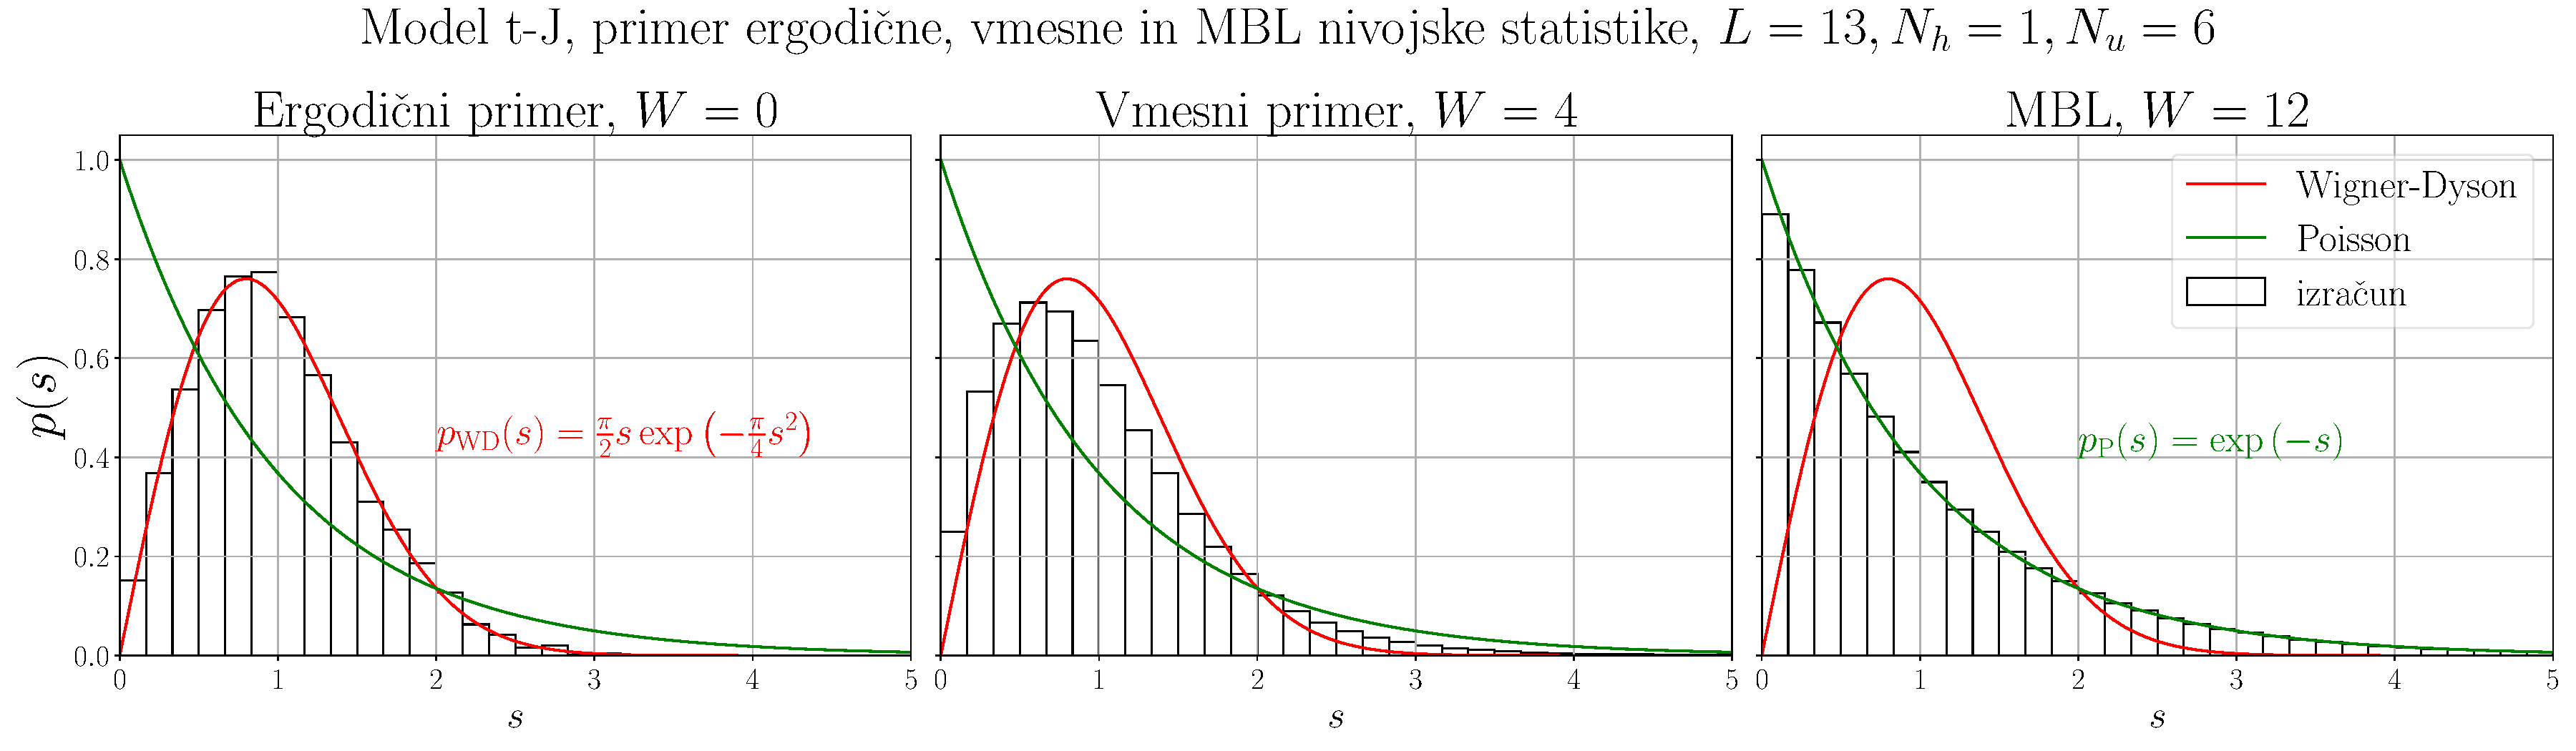
\includegraphics[trim=0 0 0 40,clip,width=1\textwidth]{unfolding_demo_three_slo.pdf}}
% \caption{$L$ - system size, $N_h$ - number of holes, $N_u$ - number of up spins.}
\end{figure}
\begin{minipage}{0.48\textwidth}
\centering \textbf{GOE:} Wigner-Dysonova porazdelitev
\end{minipage}\hfill
\begin{minipage}{0.48\textwidth}
\centering \textbf{MBL:} Poissonova porazdelitev 
\end{minipage}}
\end{frame}
\begin{frame}{Povprečno razmerje razmikov}
\begin{itemize}
	\onslide<1->{
	\item Razmiki med \textbf{sosednjimi} energijskimi nivoji:$$\delta_n=E_{n+1}-E_n \geq 0$$
	\item Definiramo \textbf{razmerje razmikov}:\vspace{3mm}
	$$0\leq r_n=\min\{\delta_n, \delta_{n-1}\}/\max\{\delta_n, \delta_{n-1}\}\leq 1$$}
	\onslide<2->{
	\item \textbf{KLJUČNO:} limitni povprečni vrednosti $\langle r \rangle$ sta dobro znani: \vspace{5mm} 
	% \begin{itemize}
		$$ \langle r \rangle_\mathrm{GOE}=0.5307, \hspace{5mm} \langle r\rangle_\mathrm{P}=2\ln2 - 1 \approx 0.3863 $$}
		% \item $\langle r \rangle_\mathrm{GOE}=0.5307$ \vspace{3mm}
		% \item $\langle r\rangle_\mathrm{P}=2\ln2 - 1 \approx 0.386$
	% \end{itemize}
\end{itemize}
\end{frame}
\begin{frame}{Rezultati}
\only<1>{
	\textbf{VPRAŠANJI:}\vspace{10mm}
	\begin{itemize}
		\item \textbf{Nastopi MBL za oba tipa nereda?}\vspace{10mm}
		\item \textbf{Kakšna je vloga dopiranja?}	
	\end{itemize}
}
\only<2,3>{
	Dopiranje z eno vrzeljo, $N_h=1$:
	\begin{figure}
	\centering{
	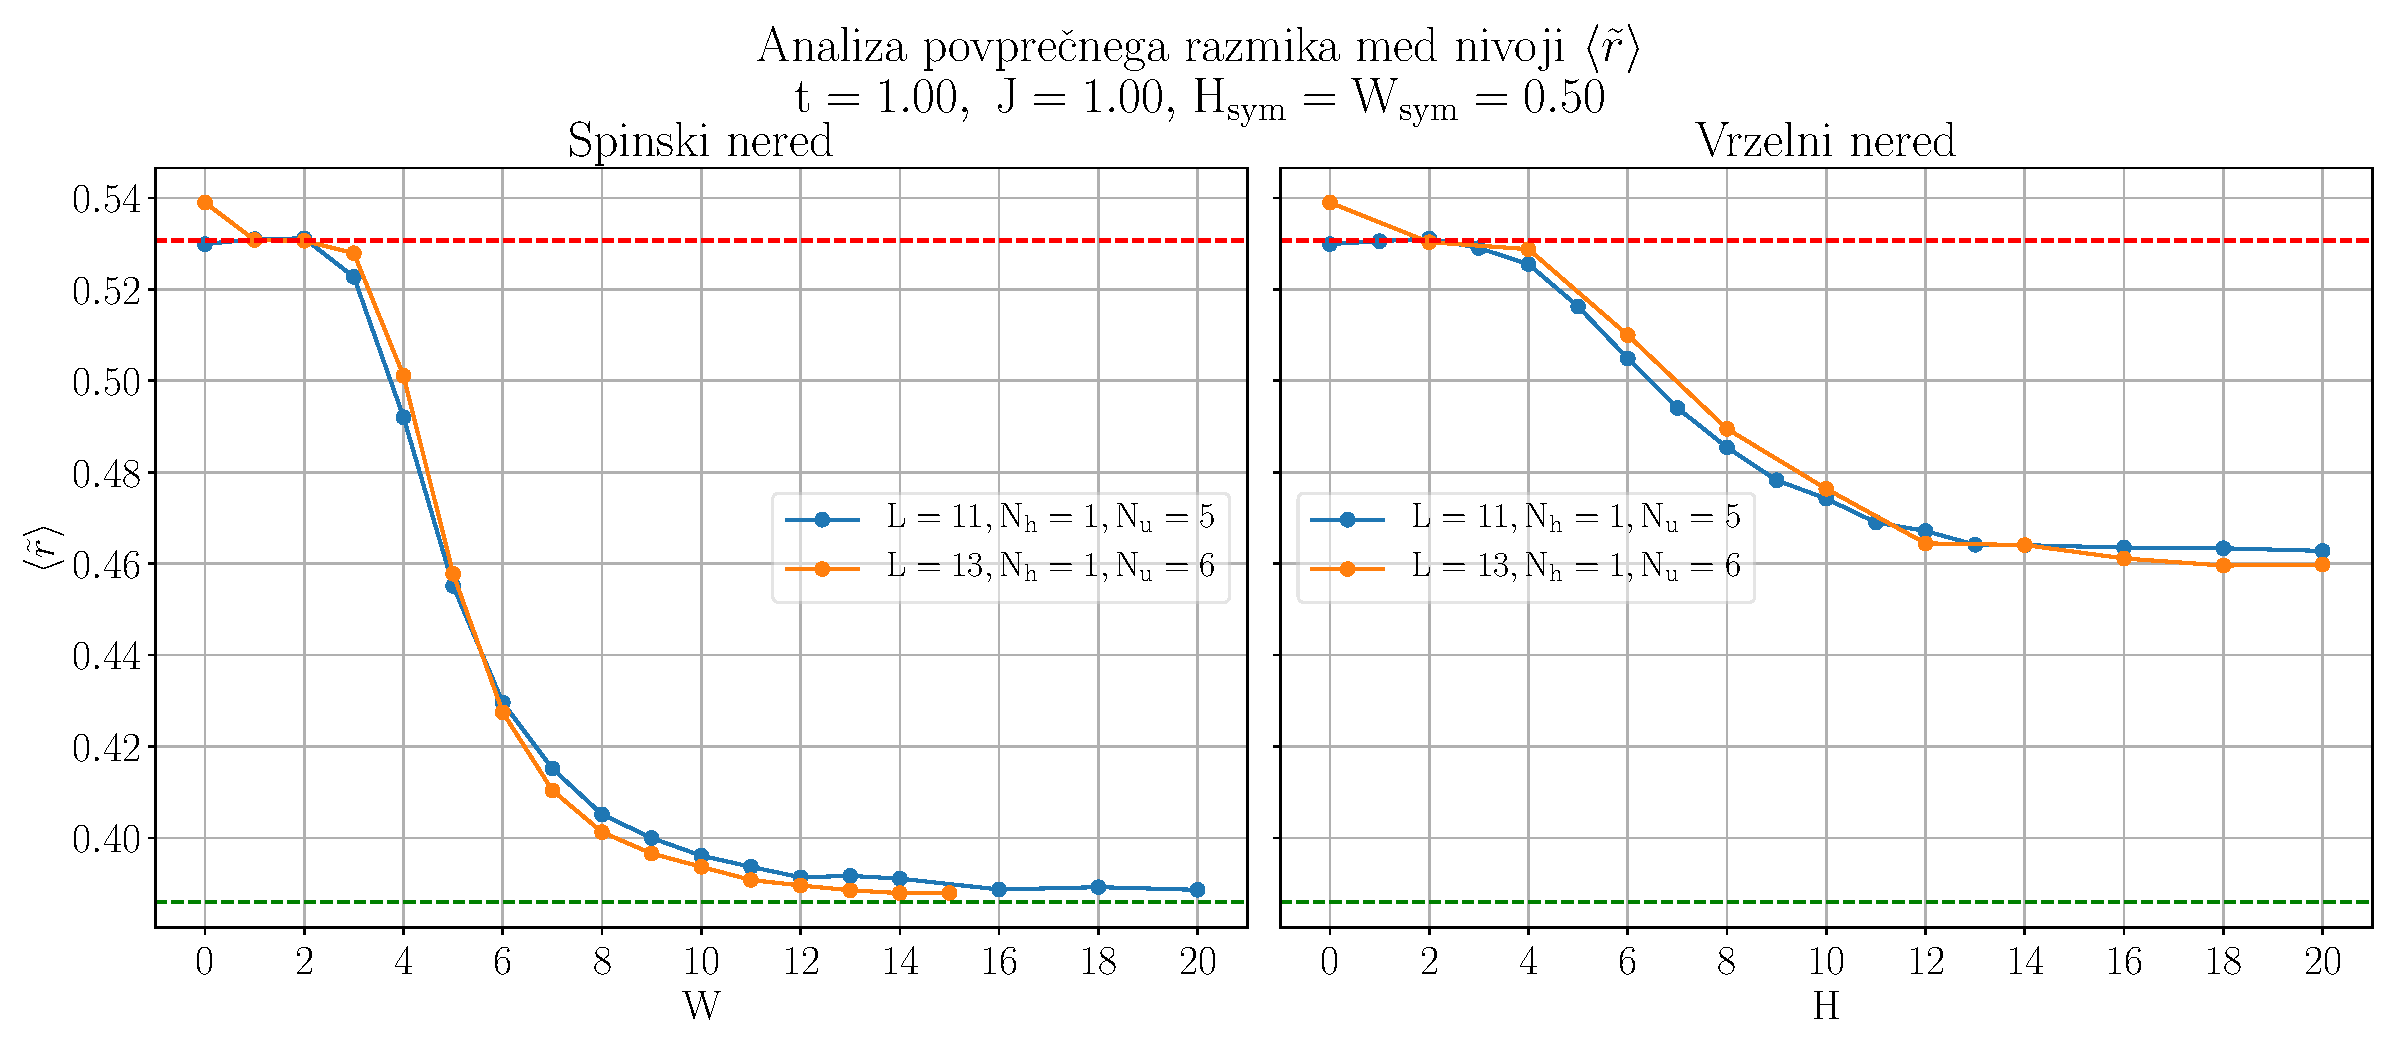
\includegraphics[trim=0 0 0 58,clip,width=1\textwidth]{double_plot_disorder_sym_break_13_1_6_slo.pdf}}
	\end{figure}
	\onslide<3->{
	\textbf{VRZELNI NERED: ni MBL}}}
\only<4,5>{
	Tretjinsko dopiranje, $N_h=L/3$:
	\begin{figure}
	\centering{
	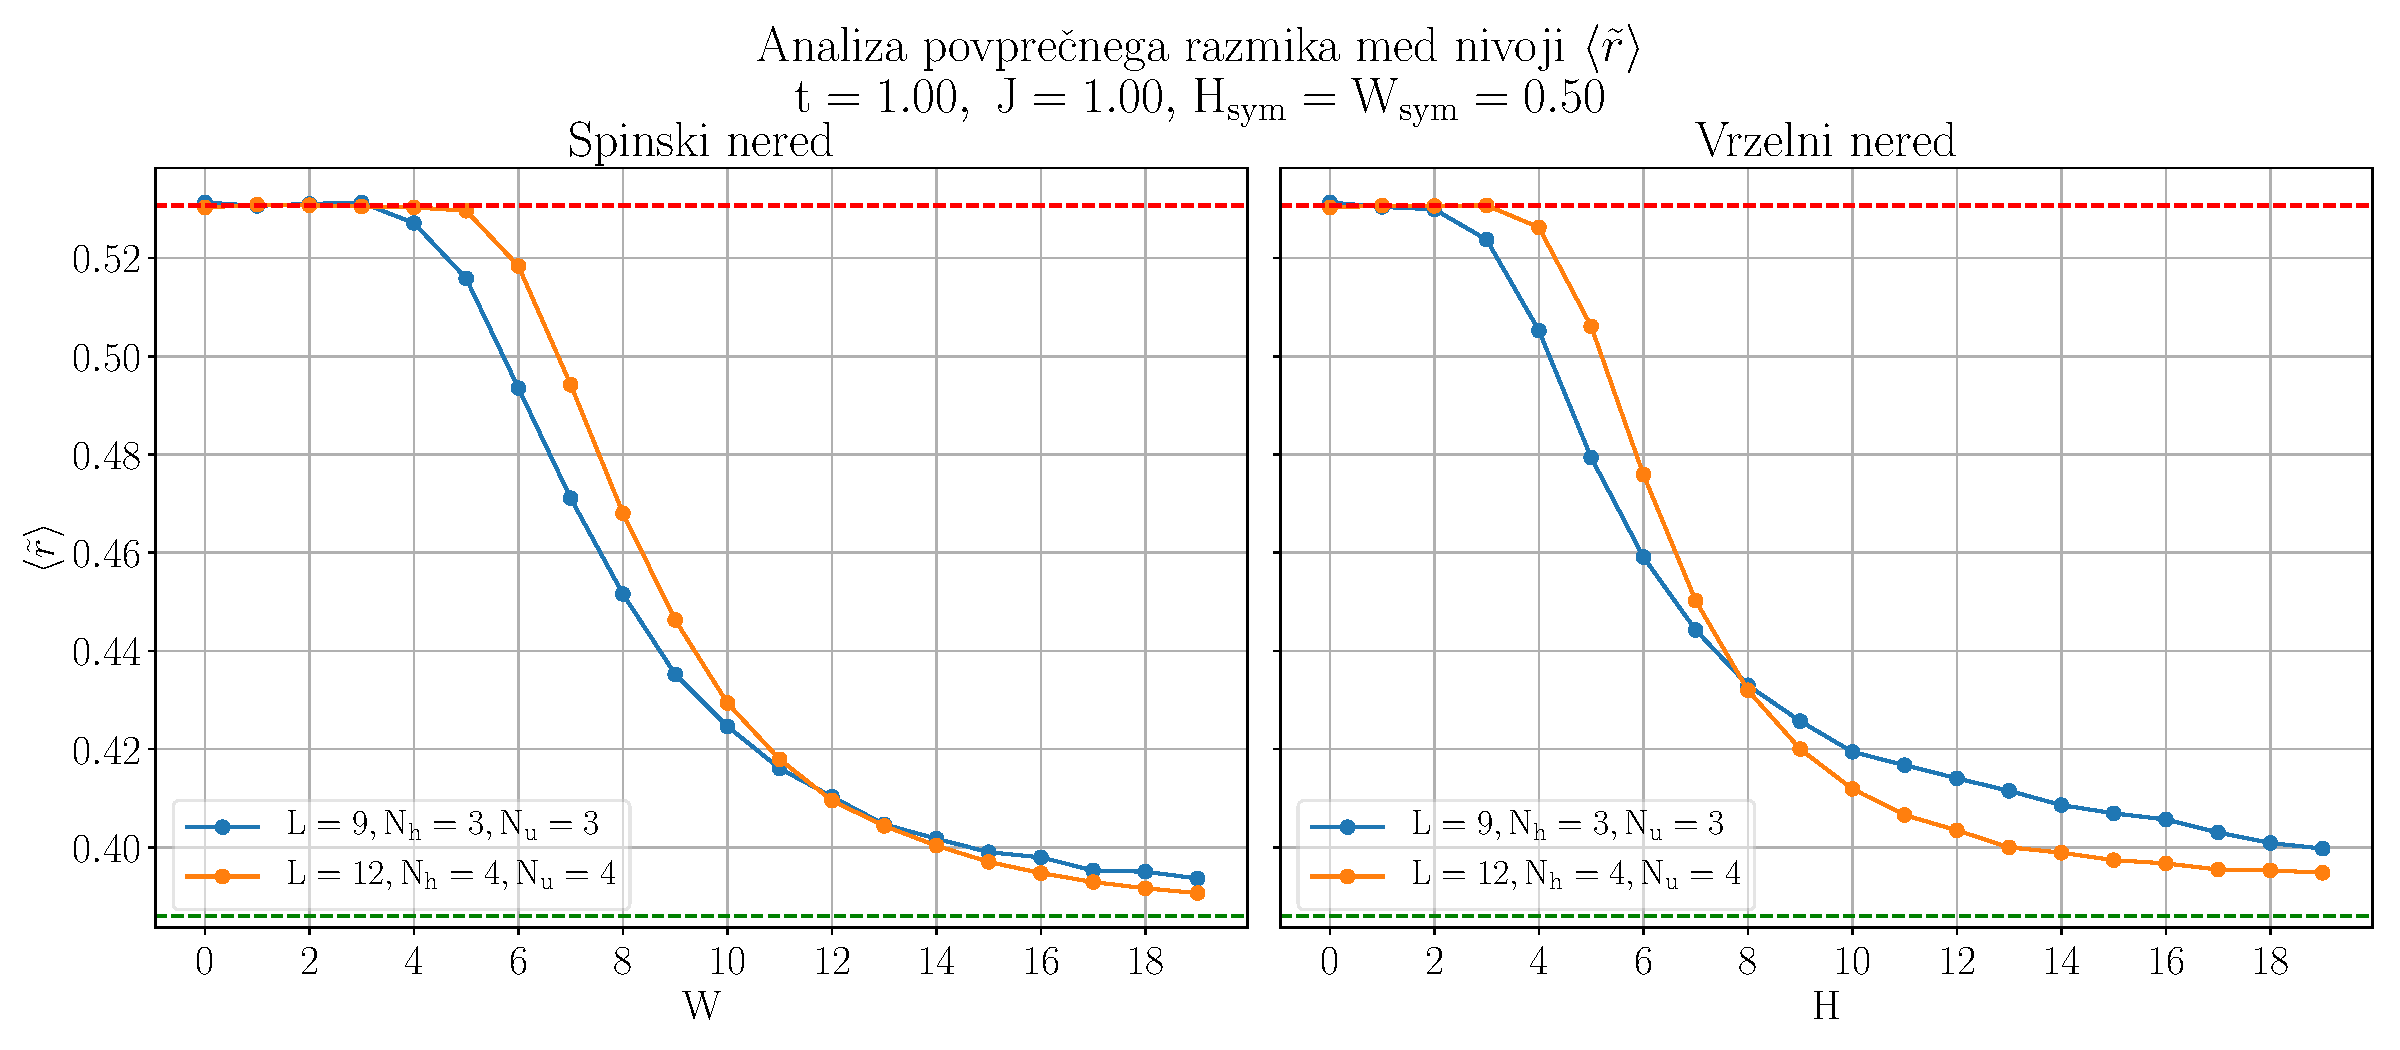
\includegraphics[trim=0 0 0 58,clip,width=1\textwidth]{double_plot_disorder_sym_break_12_4_4_slo.pdf}}
	\end{figure}
	\onslide<5->{
	\textbf{MBL za oba tipa nereda}}
}	

\only<6>{
	Oba tipa nereda hkrati\\
	\begin{minipage}[c]{0.48\textwidth}
	\begin{figure}
	\centering{
	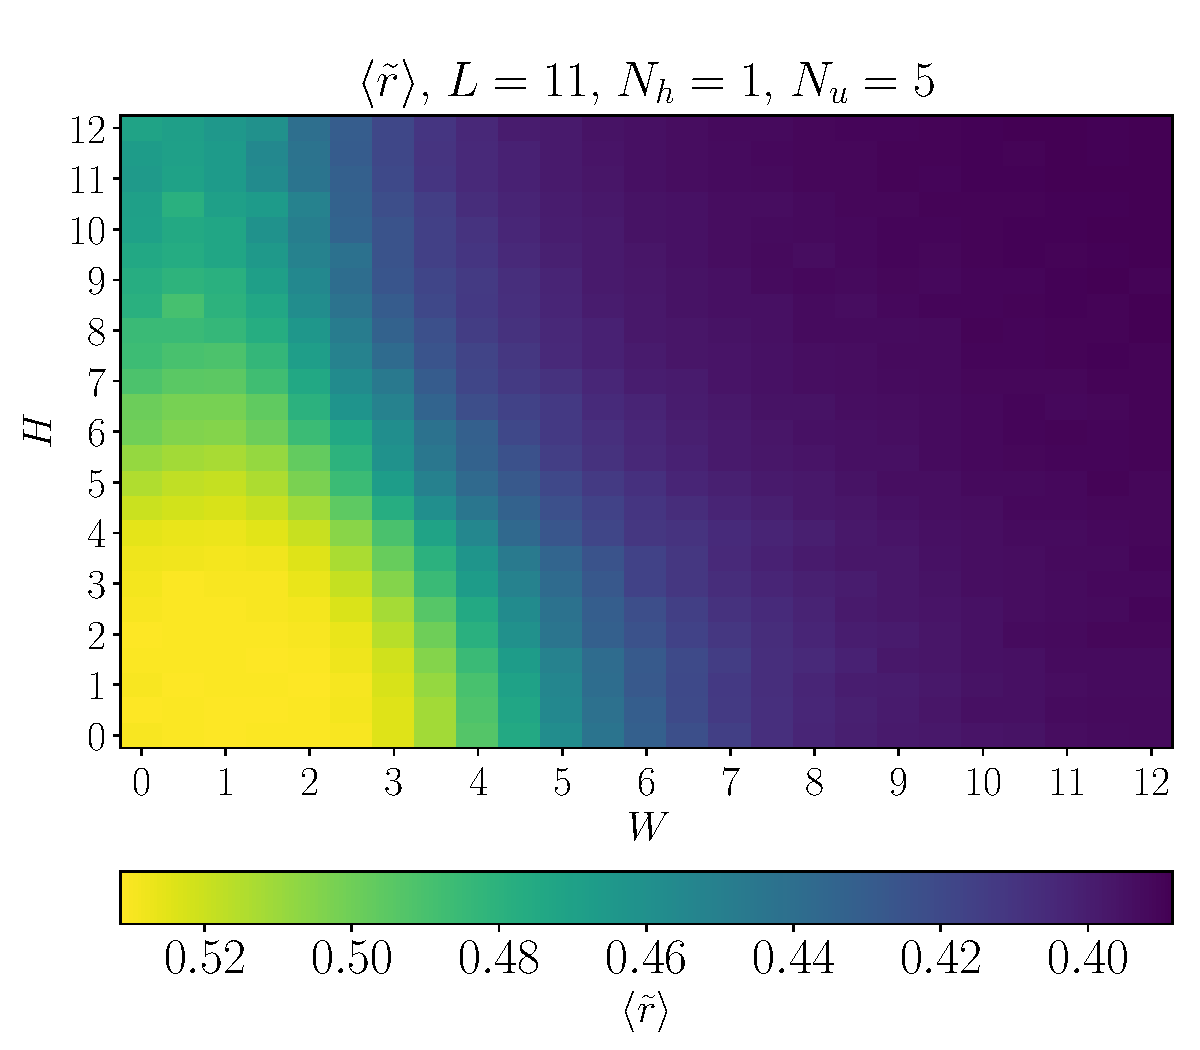
\includegraphics[width=1\textwidth]{r_density_11_1_5.pdf}}
	\caption{Ena vrzel.}
	\end{figure}
	\end{minipage}\hfill
	\begin{minipage}[c]{0.48\textwidth}
	\begin{figure}
	\centering{
	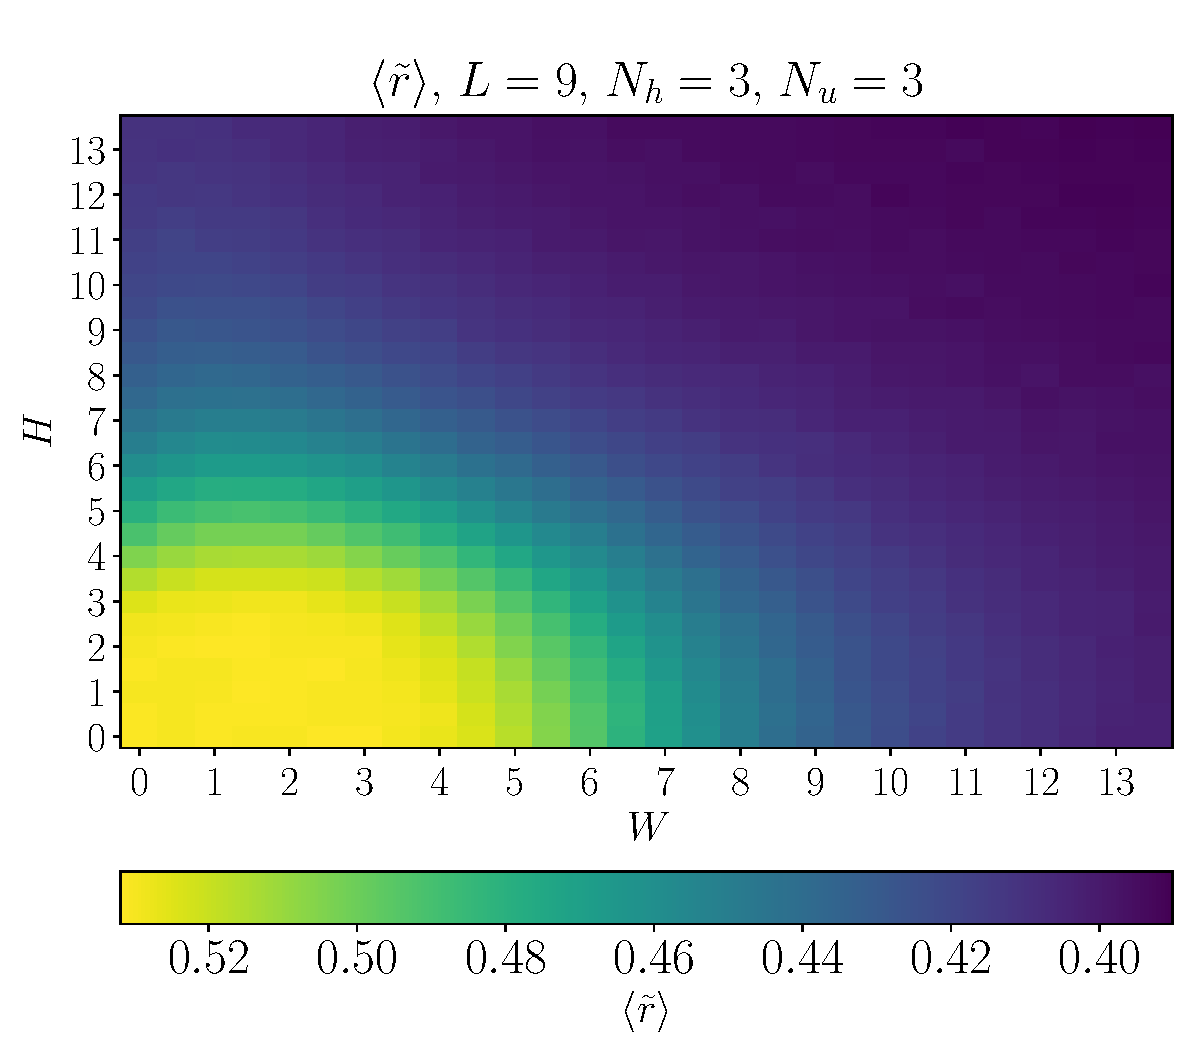
\includegraphics[width=1\textwidth]{r_density_9_3_3.pdf}}
	\caption{Tretjinsko dopiranje.}
	\end{figure}
	\end{minipage}
}



\end{frame}{}

\begin{frame}{Spektralni oblikovni faktor (SFF)}
\only<1,2>{
\begin{alertblock}{\centering{Definicija}}
$$
K(\tau)\coloneqq  \left\langle \frac{1}{N}\sum\limits_{i,j}^N \mathrm{e}^{-\iu \left(E_i - E_j\right) \tau}\right\rangle
$$
\end{alertblock}}
\only<2>{\vspace{20mm}
\begin{alertblock}{\centering{Povezani spektralni oblikovni faktor}}
$$
K_\mathrm{c}(\tau)\coloneqq  K(\tau) - \left|\left\langle \frac{1}{\sqrt{N}} \sum\limits_i \mathrm{e}^{-\iu E_i \tau}\right\rangle\right|^2
$$
\end{alertblock}}
\only<3,4>{
\begin{alertblock}{\centering{$K(\tau)$ v ergodičnem sistemu}}
\begin{equation*}\label{eq:ramp}
K_\mathrm{GOE}(\tau)=
\begin{cases}
2\tau - \tau \log\left(1 + 2\tau\right), \hspace{5mm} \tau \leq 1, \\
2 - \tau \log\left(\frac{2\tau + 1}{2\tau - 1}\right),\hspace{5mm} \tau >1.
\end{cases}
\end{equation*} 
\end{alertblock}}
\only<3>{\vspace{10mm}
\begin{alertblock}{\centering{$K(\tau)$ v MBL (in integrabilnih) sistemih}}
\begin{equation*}\label{eq:ramp}
K_\mathrm{}(\tau)=1
\end{equation*} 
\end{alertblock}
}
\only<4>{
\begin{figure}[H]
\centering{
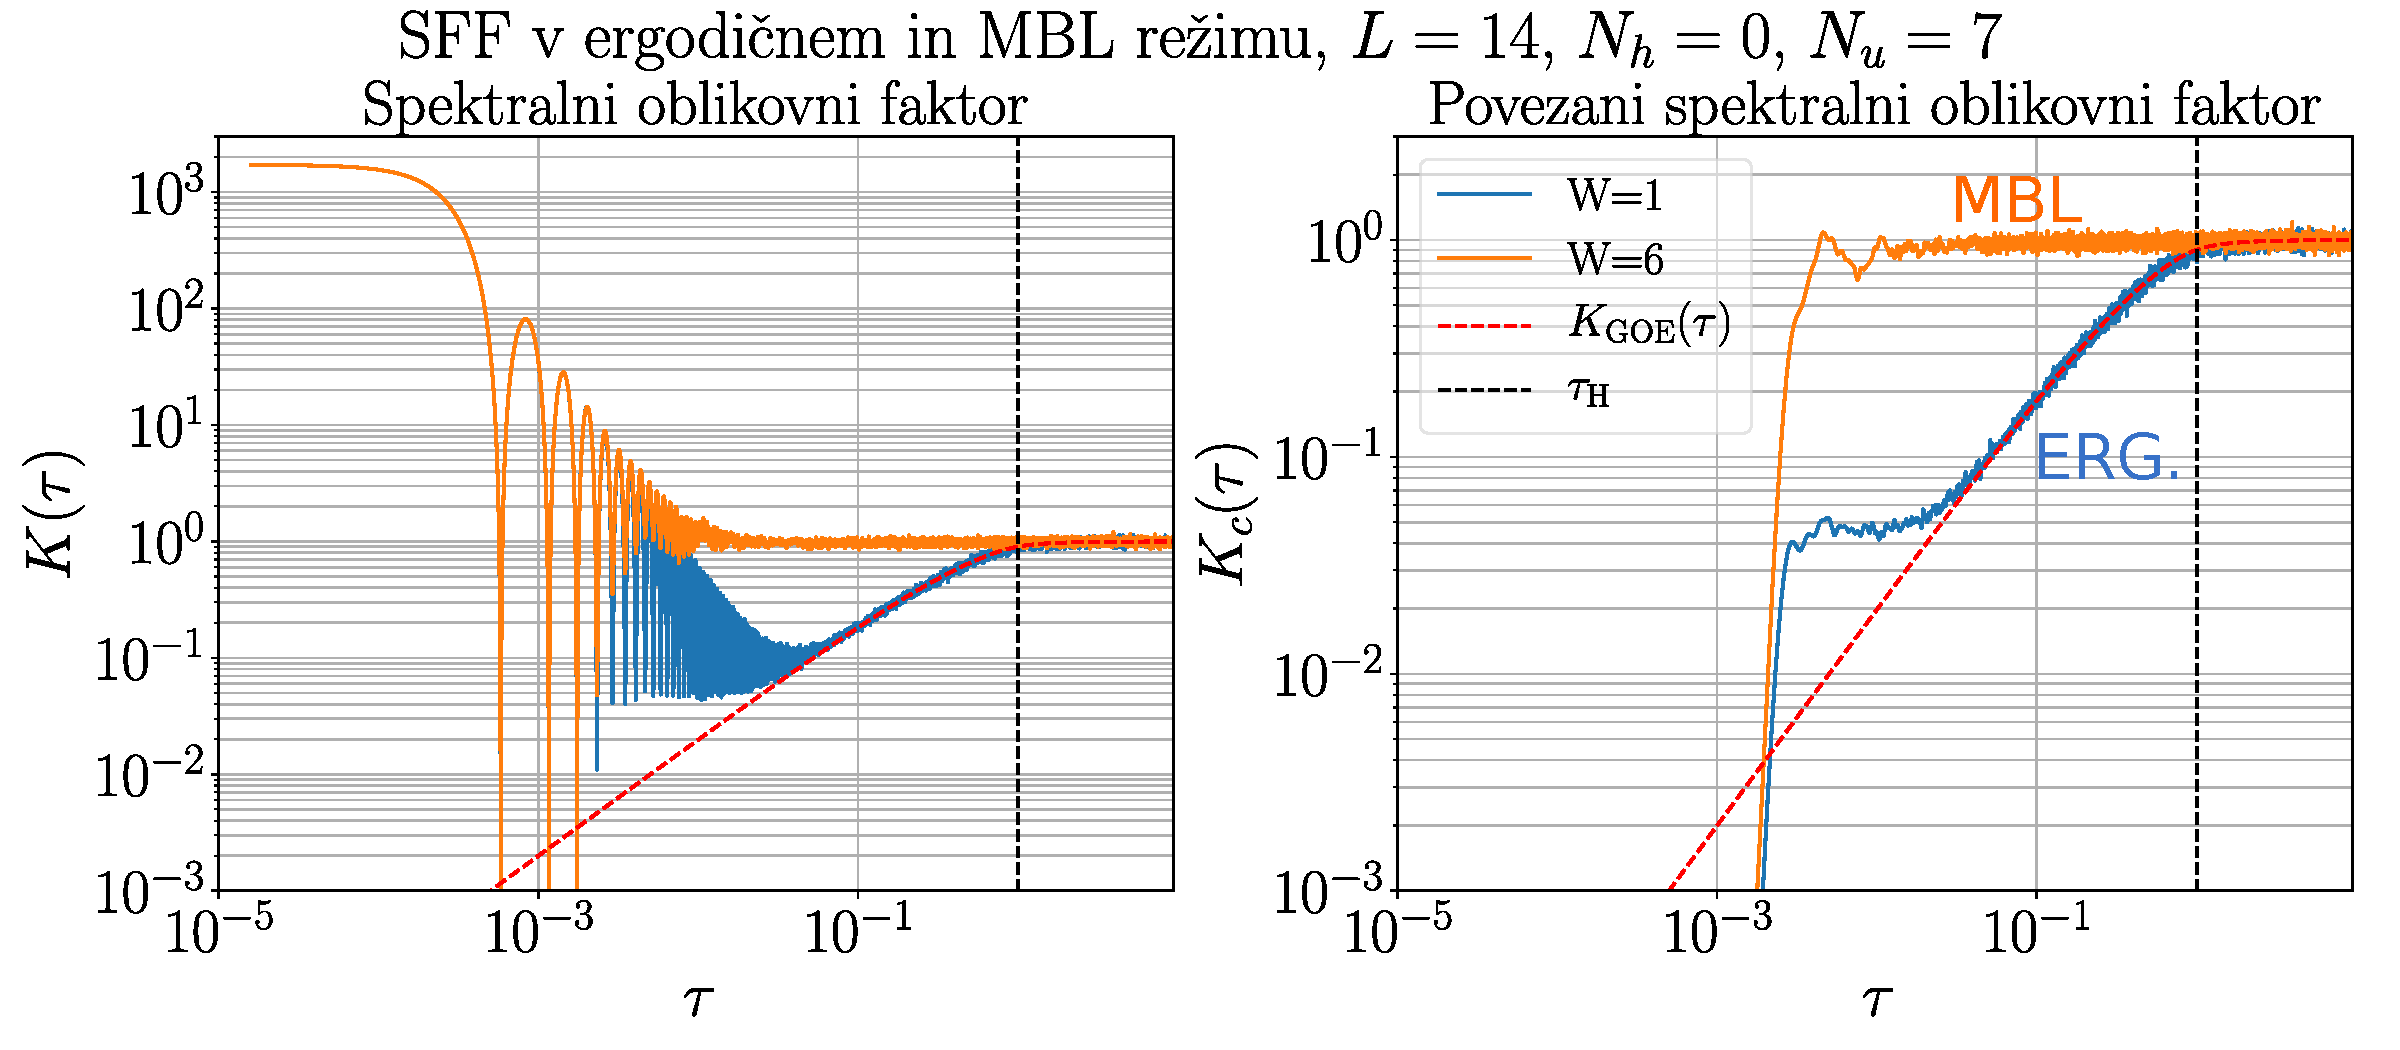
\includegraphics[width=1\textwidth]{scheme_sff_disorder_14_0_7.pdf}}
\caption{}
% \label{fig:scheme_sff_disorder_14_0_7}
\end{figure}  	
}
\end{frame}
\begin{frame}{SFF - rezultati}
\only<1,2>{
Ena vrzel - $L=11, N_h=1, N_u=5$\\\vspace{7mm}
\begin{minipage}[c]{0.48\textwidth}
\begin{figure}[H]
\centering{
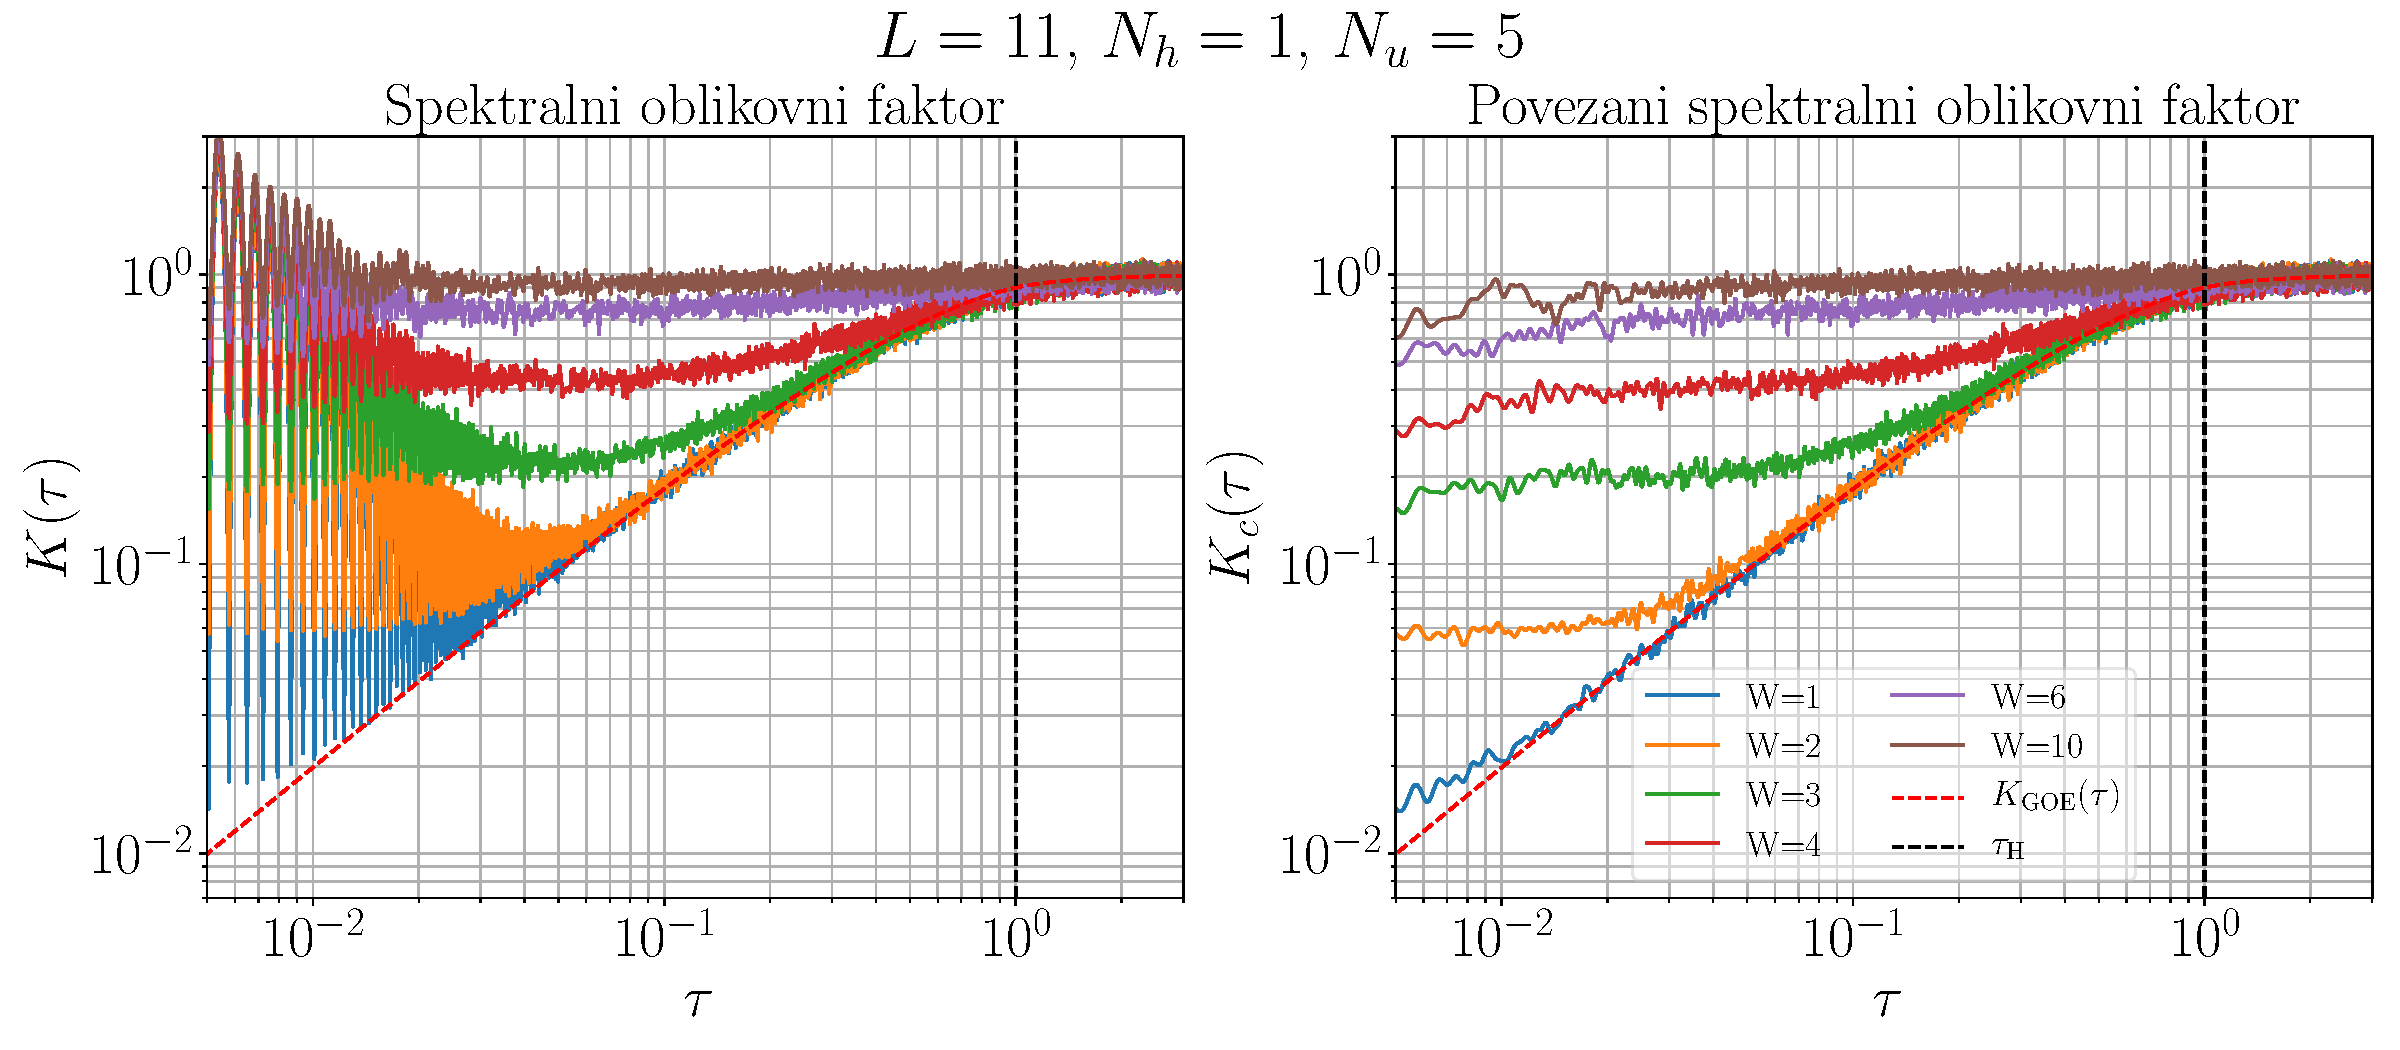
\includegraphics[trim=570 0 0 33,clip,width=1\textwidth]{W_sweep_sff_disorder_11_1_5.pdf}}
\caption{Spinski nered.}
% \label{fig:scheme_sff_disorder_14_0_7}
\end{figure} 
\end{minipage}\hfill
\begin{minipage}[c]{0.48\textwidth}
\begin{figure}[H]
\centering{
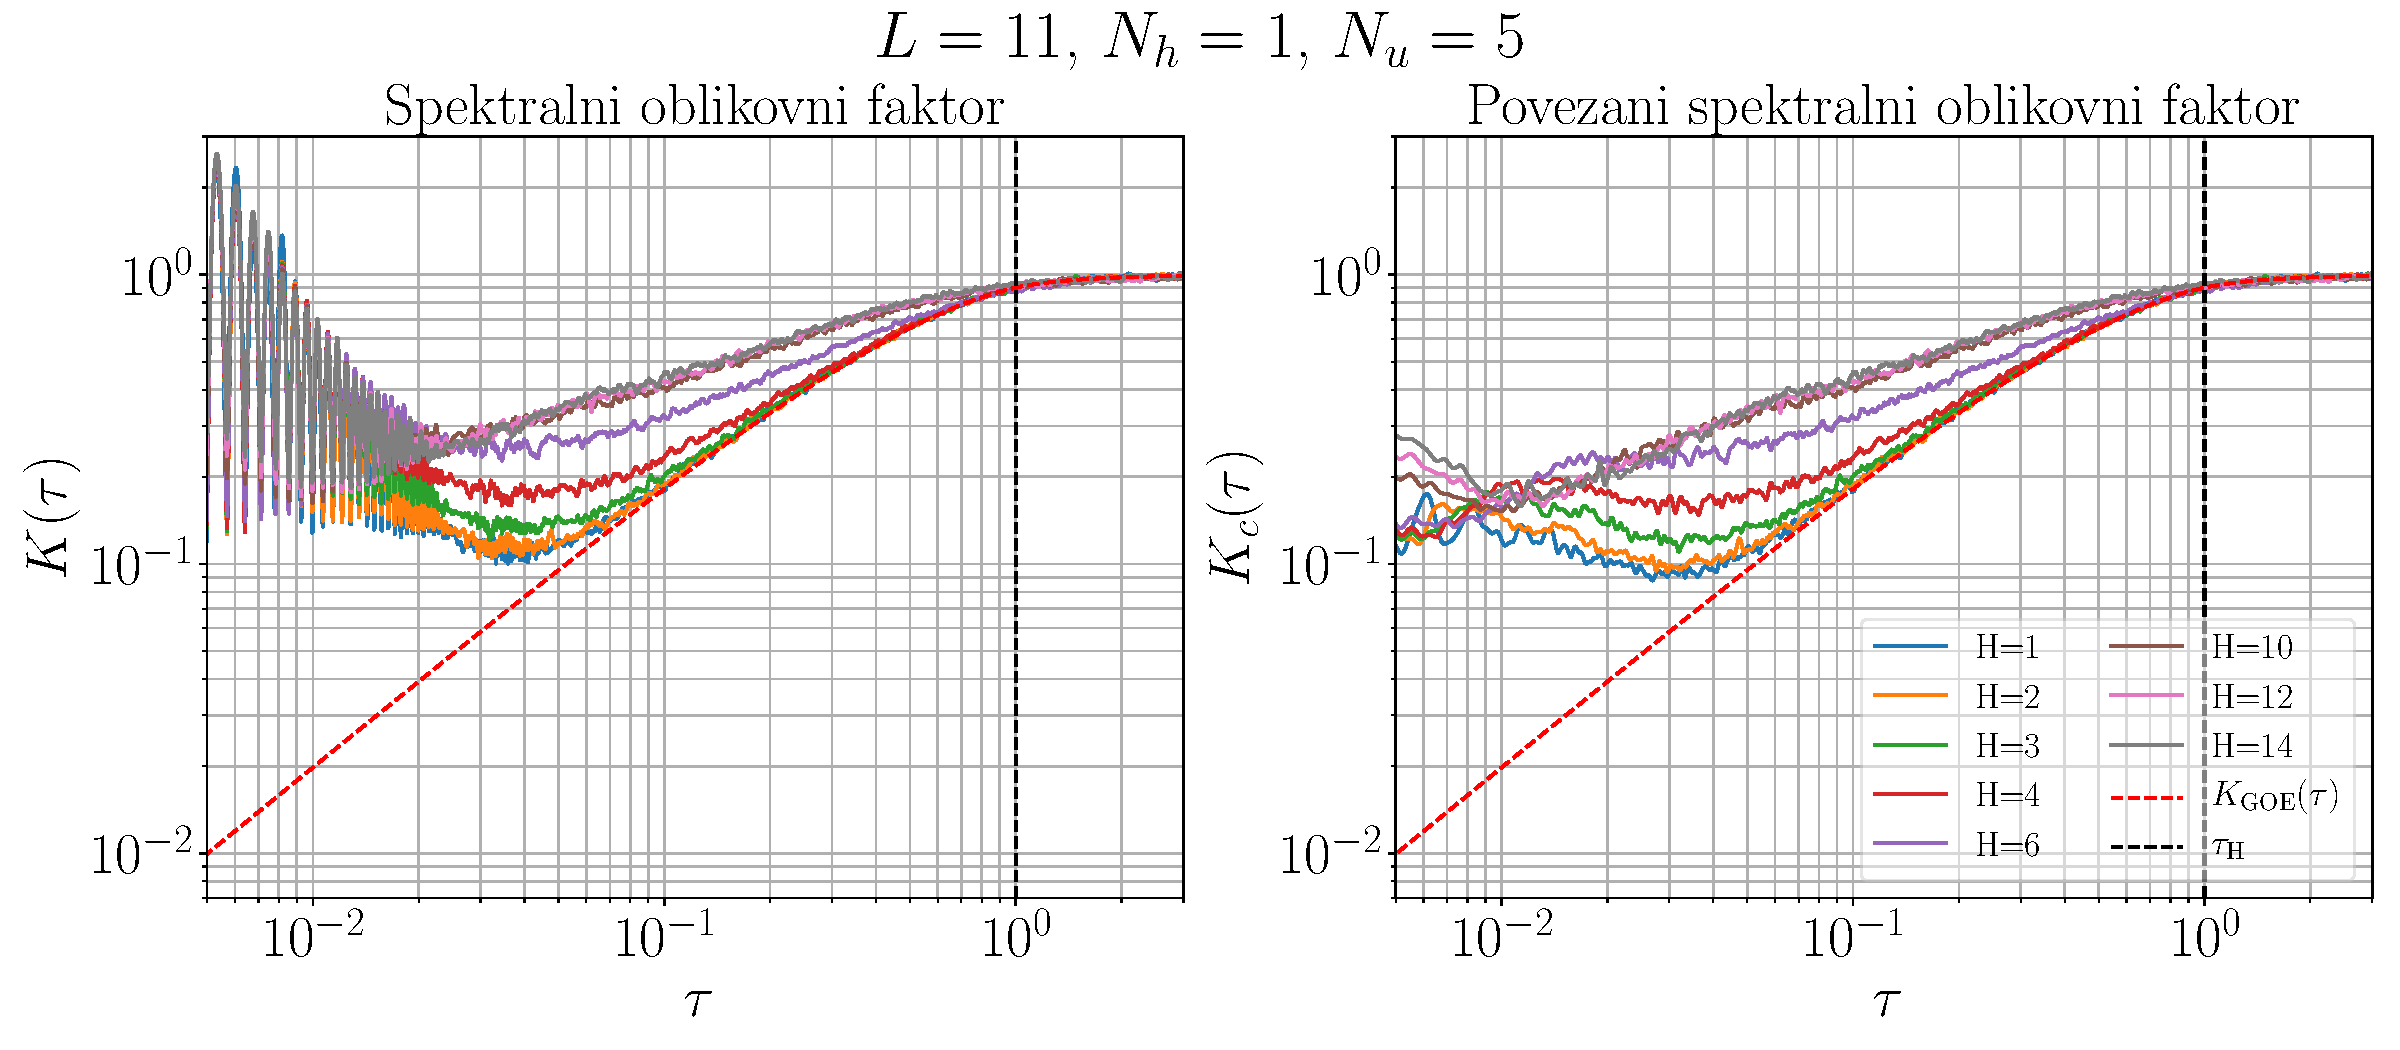
\includegraphics[trim=570 2 0 33,clip,width=1\textwidth]{H_sweep_sff_disorder_11_1_5.pdf}}
\caption{Vrzelni nered - \textbf{ni MBL}.}
% \label{fig:scheme_sff_disorder_14_0_7}
\end{figure} 
\end{minipage}
}
\only<2>{\textbf{Za vrzelni nered NI PREHODA - vmesno obnašanje.}}
\only<3,4>{
Tretjinsko dopiranje - $L=9, N_h=3, N_u=3$\vspace{7mm}
\begin{minipage}[c]{0.48\textwidth}
\begin{figure}[H]
\centering{
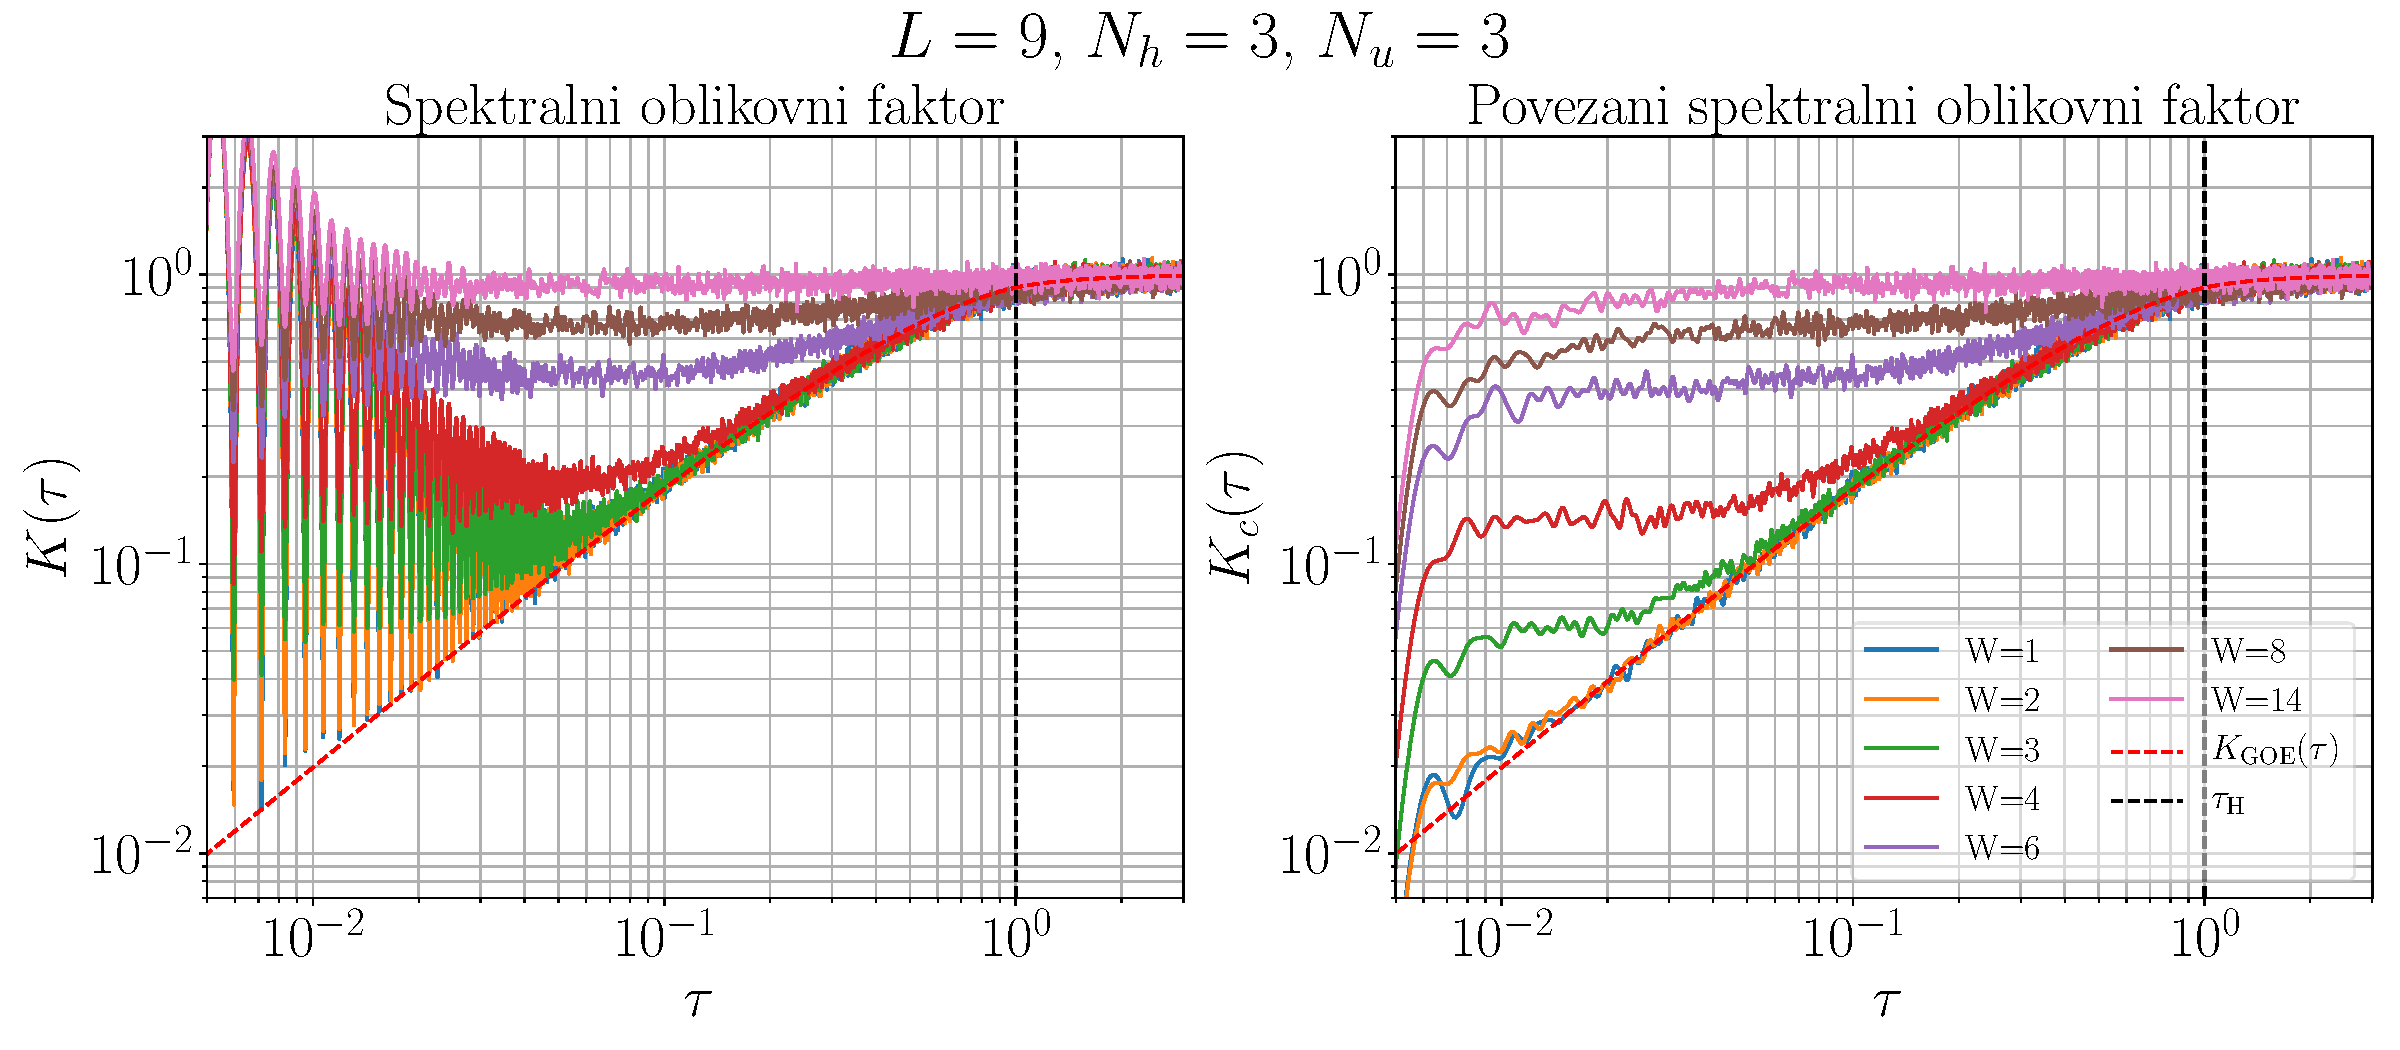
\includegraphics[trim=570 0 0 33,clip,width=1\textwidth]{W_sweep_sff_disorder_9_3_3.pdf}}
\caption{Spinski nered.}
% \label{fig:scheme_sff_disorder_14_0_7}
\end{figure} 
\end{minipage}\hfill
\begin{minipage}[c]{0.48\textwidth}
\begin{figure}[H]
\centering{
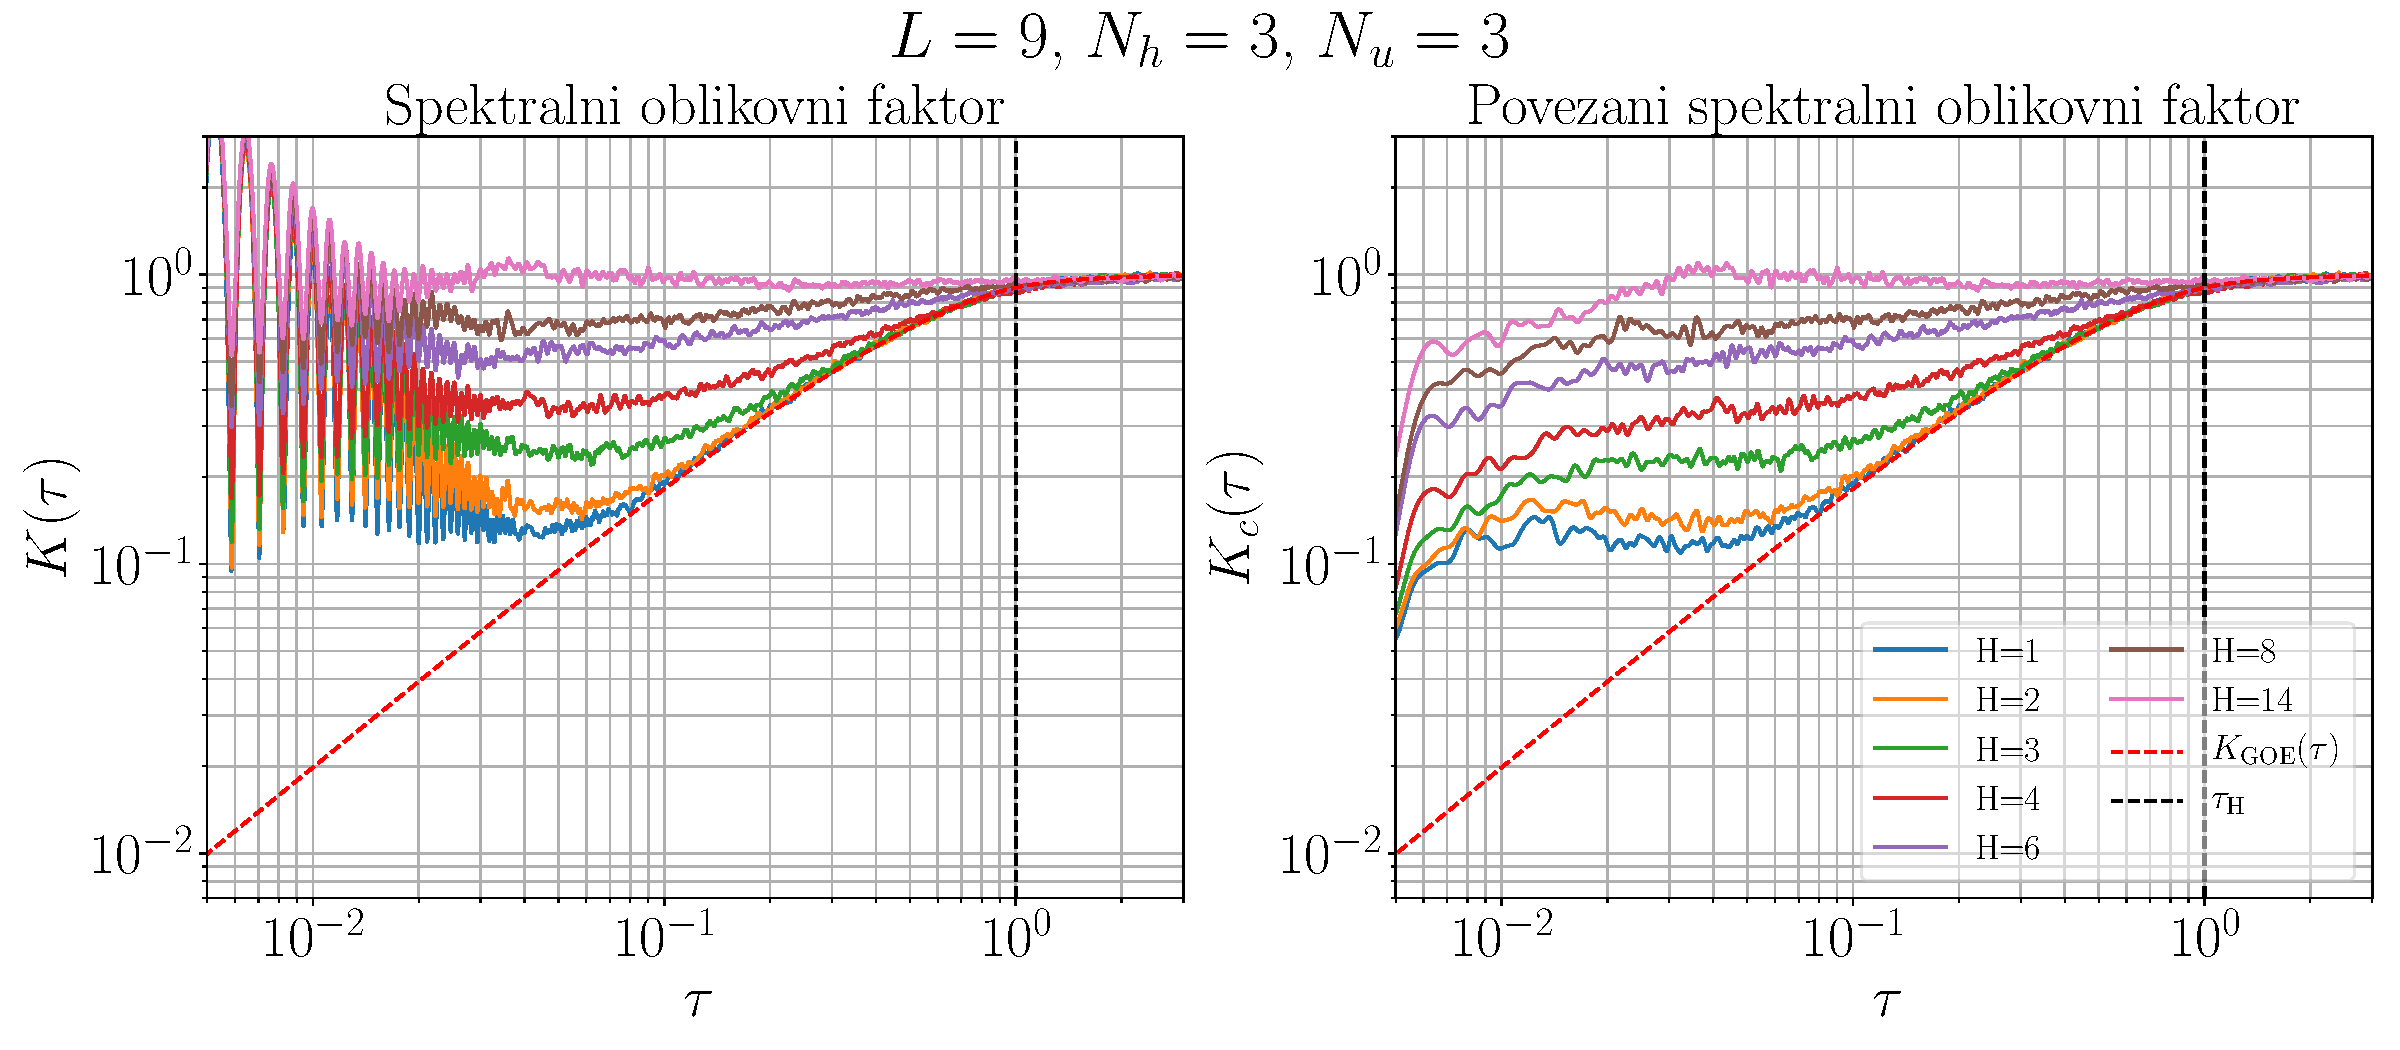
\includegraphics[trim=570 2 0 33,clip,width=1\textwidth]{H_sweep_sff_disorder_9_3_3.pdf}}
\caption{Vrzelni nered.}
% \label{fig:scheme_sff_disorder_14_0_7}
\end{figure} 
\end{minipage}
}
\only<4>{\textbf{Prehod v MBL za oba tipa nereda.}}

\end{frame}






% \begin{frame}{Anderson localization}
% What began in 1958 ...
% \only<1->{\begin{figure}
% \centering{
% 
\includegraphics[width=0.9\textwidth]{and_orig_crop.pdf}}
% % \caption{}
% \end{figure}}
% \only<2->{
% ... still remains relevant today
% \begin{figure}
% \centering{
% 
\includegraphics[width=0.8\textwidth]{huse_crop.pdf}}
% % \caption{}
% \end{figure}}
% \end{frame}
% \begin{frame}{MBL - the current ``hot topic''}
% % \begin{itemize}
% % % \item \textbf{Many-body localization (MBL)} - includes \textbf{INTERACTIONS}
% % \vspace{10mm}
% % \end{itemize}
% \begin{minipage}[c]{0.6\textwidth}
% Published in 2015:
% \begin{figure}
% \centering{
% 
\includegraphics[width=1\textwidth]{mbl_crop.pdf}}
% \caption{672 citations as of April 2018 acc. to Google Scholar.}
% \end{figure}
% \end{minipage}
% % \begin{minipage}[c]{0.38\textwidth}
% % \begin{itemize}
% % \vspace{5mm}
% % \item not our today's topic
% % \end{itemize}
% % \end{minipage}
% \end{frame}



% \begin{frame}{What is Anderson localization all about?}
% \begin{minipage}[c]{0.9\textwidth}
% \begin{itemize}
% \item Conduction in \textbf{NON-INTERACTING} systems with \textbf{DISORDER}
% \vspace{15mm}
% \item Describes the role of \textbf{IMPURITIES}
% \vspace{15mm}
% \item Completely different than the \textbf{Drude} model:
% $$ \sigma \propto l, \hspace{10mm} l: \text{the mean-free path}$$
% \end{itemize}
% \end{minipage}
% \end{frame}

% \begin{frame}{Anderson localization - the predictions}
% \only<1->{
% \centering{
% \begin{itemize}
% \item for some disorder: \hspace{5mm}
% $ \sigma = 0$ \vspace{5mm}
% \item seminal paper by \textbf{P. W. Anderson (1958)} \cite{Anderson}\vspace{5mm}
% \item Nobel prize in \textbf{1977}
% \end{itemize}}\vspace{2mm}}
% \only<2->{
% \begin{minipage}[c]{0.94\textwidth}

% \begin{figure}
% \centering{
% 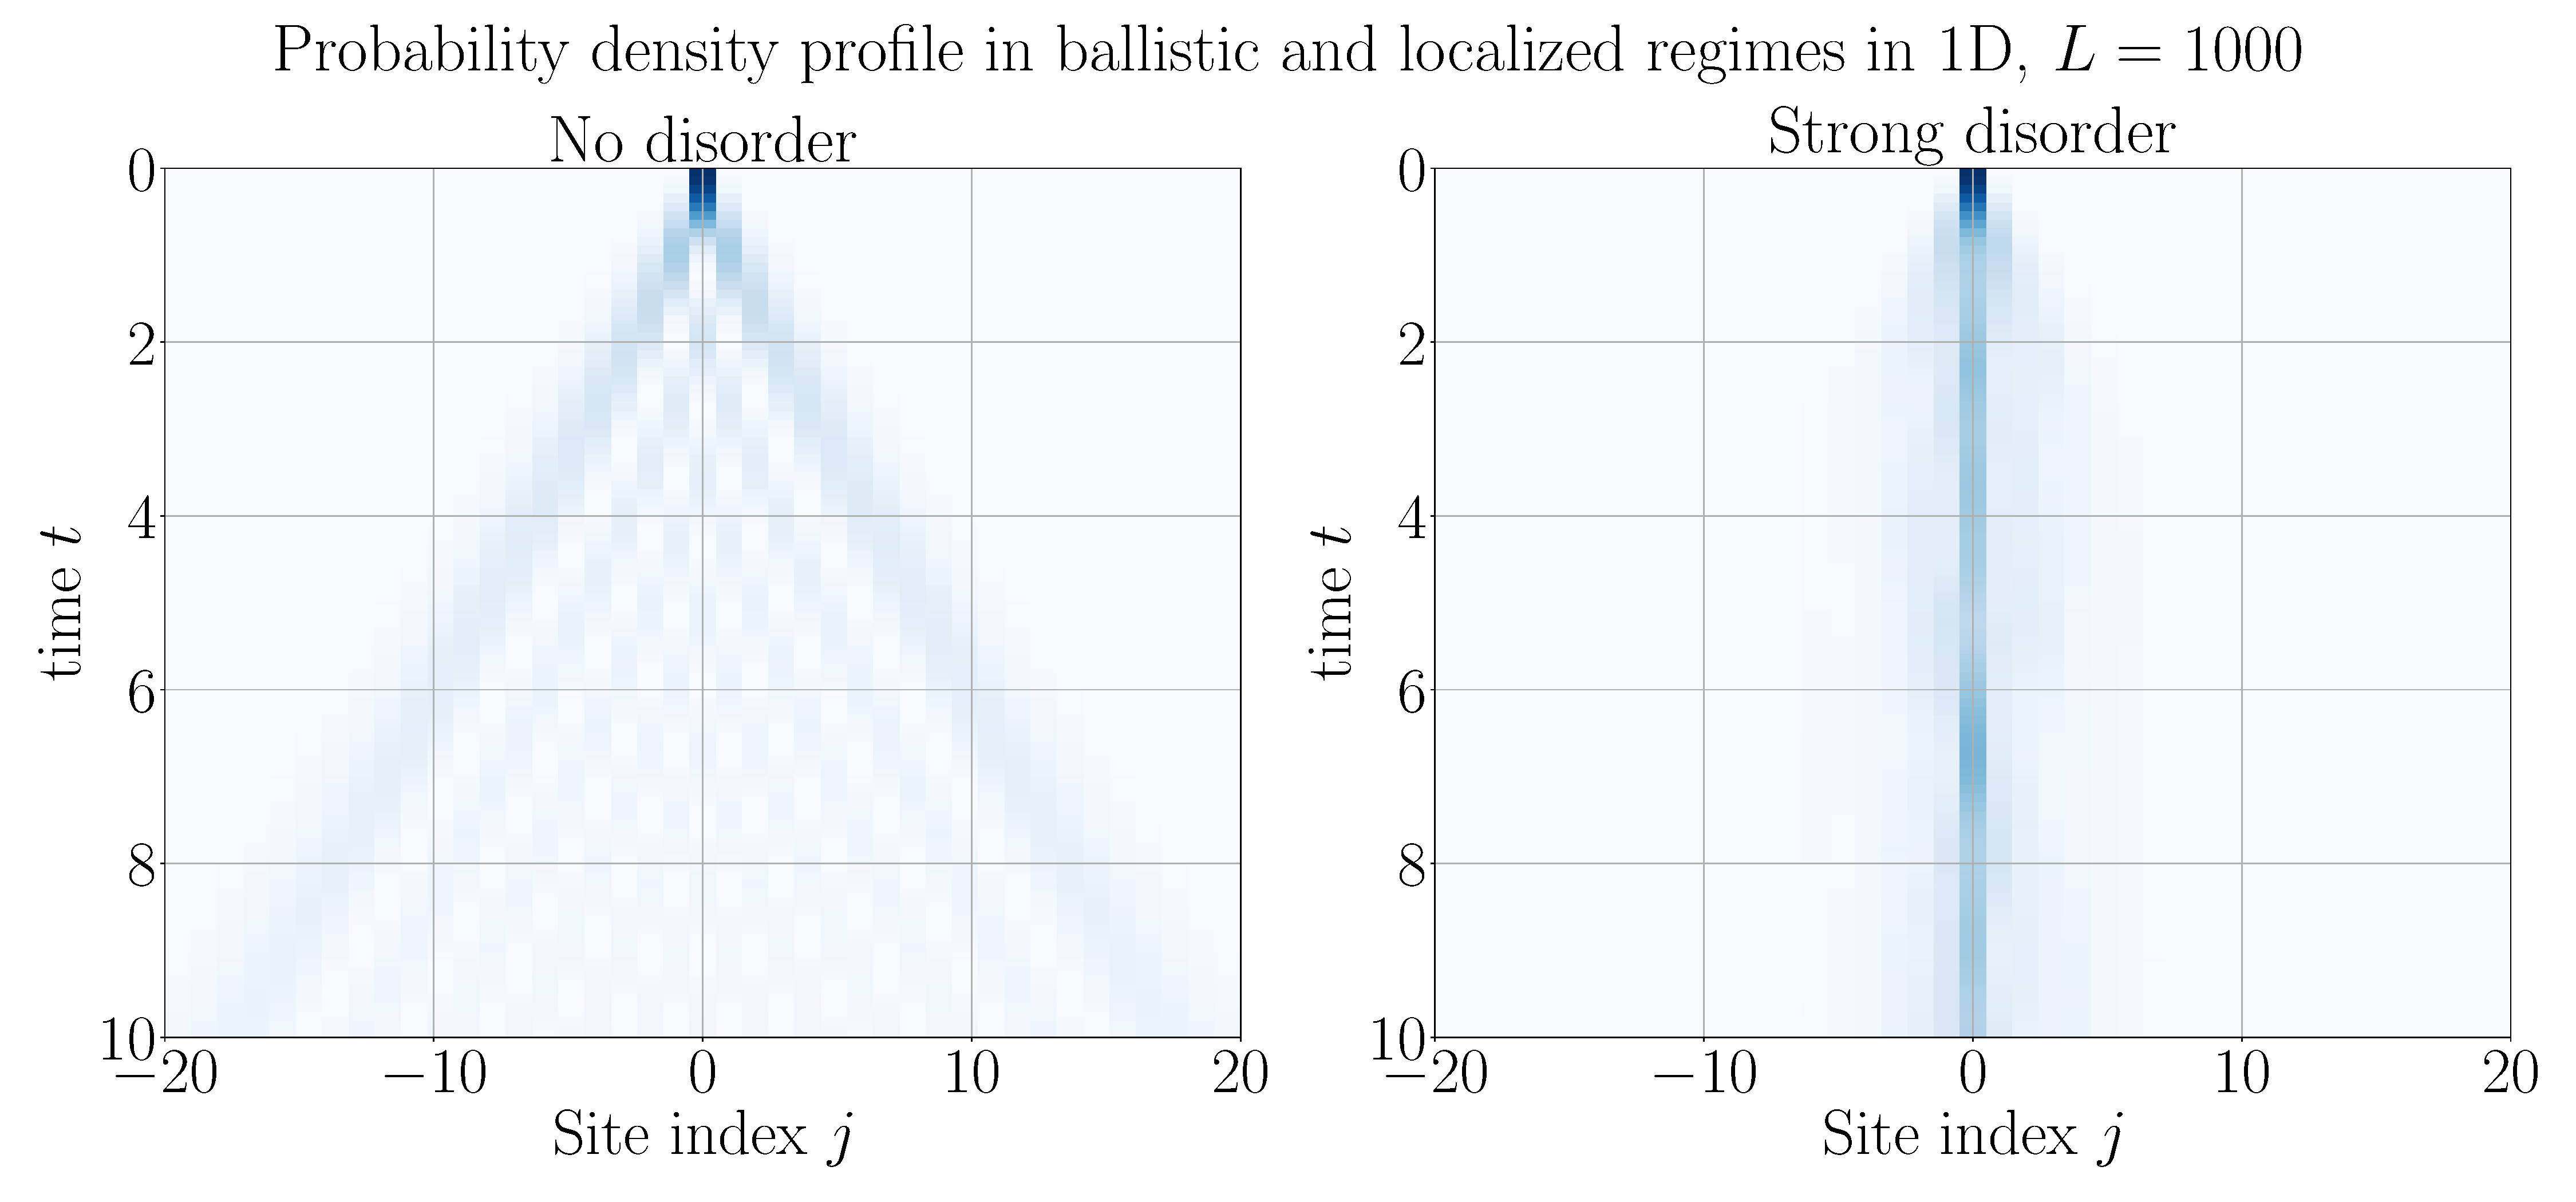
\includegraphics[width=1\textwidth]{1D_Anderson_localization_Seminar_scaling_analysis_D1_shape_1000_light_cone_double_presentation.pdf}}
% % \caption{1D dynamics with no disorder and with strong disorder.}
% \end{figure}
% \end{minipage}}
% \end{frame}



% % \begin{frame}{The model in a nutshell}
% % % \begin{alertblock}{The model Hamiltonian}
% % % \begin{equation*}\label{eq:ising_hamiltonian}
% % % H_I=-J\sum\limits_i \hat{\sigma}_i^z\hat{\sigma}_{i+1}^z - h_{\perp}\sum\limits_i \hat{\sigma}_{i}^x.
% % % \end{equation*}
% % % \end{alertblock}{}

% % % \begin{minipage}[c]{0.49\textwidth}
% % % \begin{figure}
% % % \centering{
% % % \includegraphics[width=1\textwidth]{Sachdev_phase_diagram.pdf}}
% % % \caption{The phase diagram.}
% % % \end{figure}
% % % \end{minipage}
% % % \begin{minipage}[c]{0.4\textwidth}
% % % \begin{figure}
% % % \centering{
% % % \includegraphics[width=1\textwidth]{zigzag_chain.jpg}}
% % % \caption{The schematic of cobalt niobate}
% % % \end{figure}
% % % \end{minipage}\hfill

% % \end{frame}

% \begin{frame}{The basics}
% \begin{minipage}[c]{0.5\textwidth}
% \begin{itemize}
% \item \textbf{DISORDER} $\rightarrow$ \textbf{(eigen)}states can localize
% \vspace{10mm}
% \item A localized state:
% $$|\psi(\mathbf{r})| \sim \exp\left(|\mathbf{r} - \mathbf{r}_0 |/\xi \right)$$
% \vspace{5mm}
% \item explains \textbf{vanishing} transport
% \vspace{10mm}
% % \item An \textbf{interference} phenomenon.
% \end{itemize}
% \end{minipage}
% \begin{minipage}[c]{0.4\textwidth}
% \centering
% Localization:
% \begin{figure}
% \centering{
% 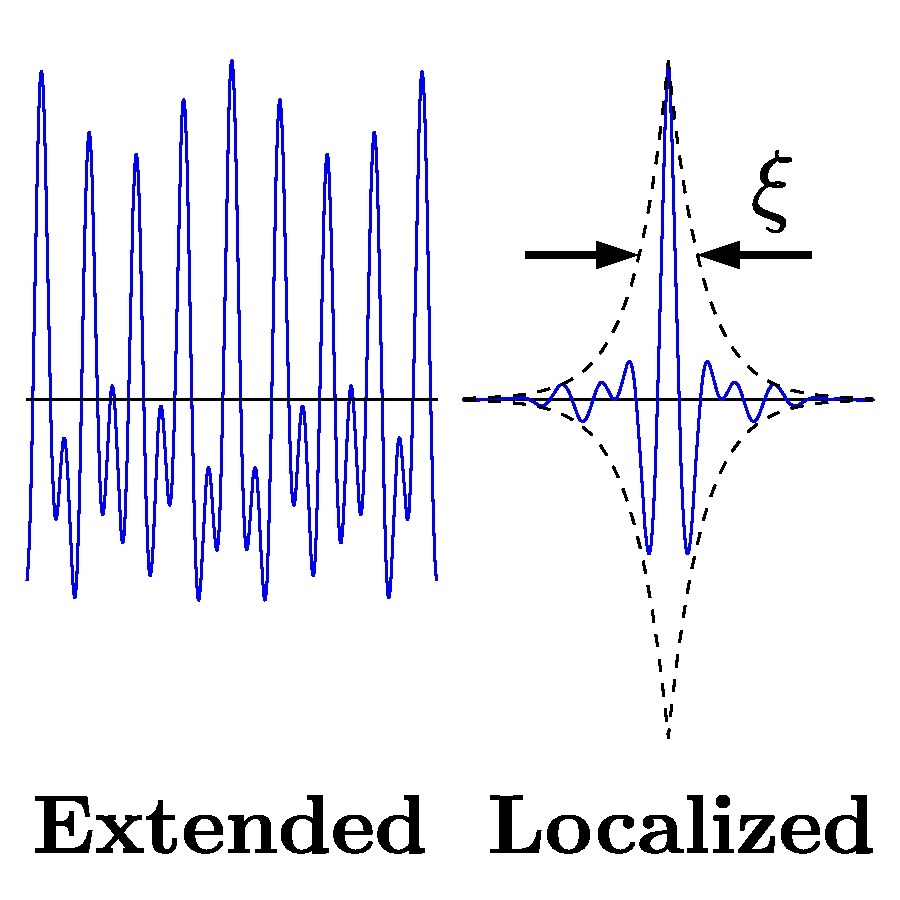
\includegraphics[width=1\textwidth]{diff_loc_ext1_modified.pdf}}
% % \caption{Extended and localized states.}
% \end{figure}
% \end{minipage}
% \end{frame}

% \begin{frame}{The important keynotes}
% \begin{minipage}[c]{0.9\textwidth}
% \begin{itemize}
% \item An \textbf{interference} phenomenon
% \vspace{12mm}		
% \item Strong \textbf{dimensionality} dependence
% \vspace{12mm}
% \item Energy dependence $\rightarrow$ the \textbf{mobility edge}

% % USE THIS LAST BULLET POINT TO INTRODUCE THE NEXT SLIDE
% \end{itemize}
% \end{minipage}
% \end{frame}


% \begin{frame}{The scaling theory  }
% \begin{itemize}
% \item scaling of the \textbf{conductance} $g$ of 
% a \textbf{hypercube} $L^d$ \vspace{3mm} \cite{scaling}
% \end{itemize}
% \begin{minipage}[c]{0.38\textwidth}
% \begin{itemize}
% % \vspace{15mm}
% \onslide<2->{\item \textbf{Ohmic} conductor:
% $$g=\sigma L^{d-2}$$}
% \vspace{5mm} 
% \onslide<3->{\item \textbf{Localized} regime:
% $$g\propto \exp(-L)$$}
% % \item \textbf{QPT} at $h_{\perp_c}=J$
% \end{itemize}
% \end{minipage}\hfill
% \begin{minipage}[c]{0.6\textwidth}
% \begin{figure}
% \centering{
% 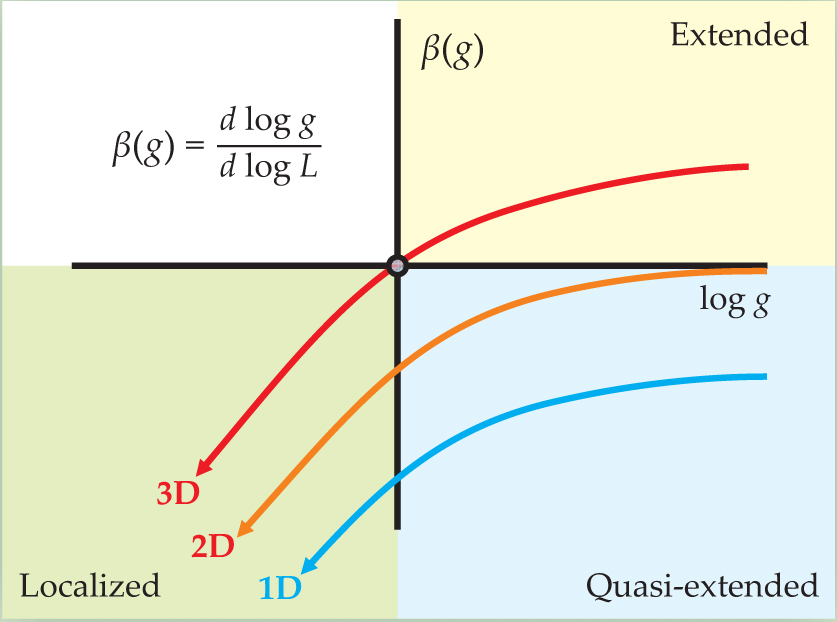
\includegraphics[width=1\textwidth]{beta_diagram.jpg}}
% \caption{Transition between ext. and loc. states is only possible in 3D. Taken from \cite{50yearsof}.}
% \end{figure}
% \end{minipage}
% \end{frame}
% \begin{frame}{The scaling theory}
% \begin{minipage}[c]{0.36\textwidth}
% \begin{alertblock}{\centering\textbf{1D, 2D}}
% \centering localization for any finite disorder
% \end{alertblock}\vspace{0.65cm}
% \begin{alertblock}{\centering\textbf{3D}}
% \centering localization for some critical disorder
% \end{alertblock}\vspace{0.35cm}
% \end{minipage}\hfill
% \begin{minipage}[c]{0.6\textwidth}
% \vspace{5mm}
% \begin{figure}
% \centering{
% 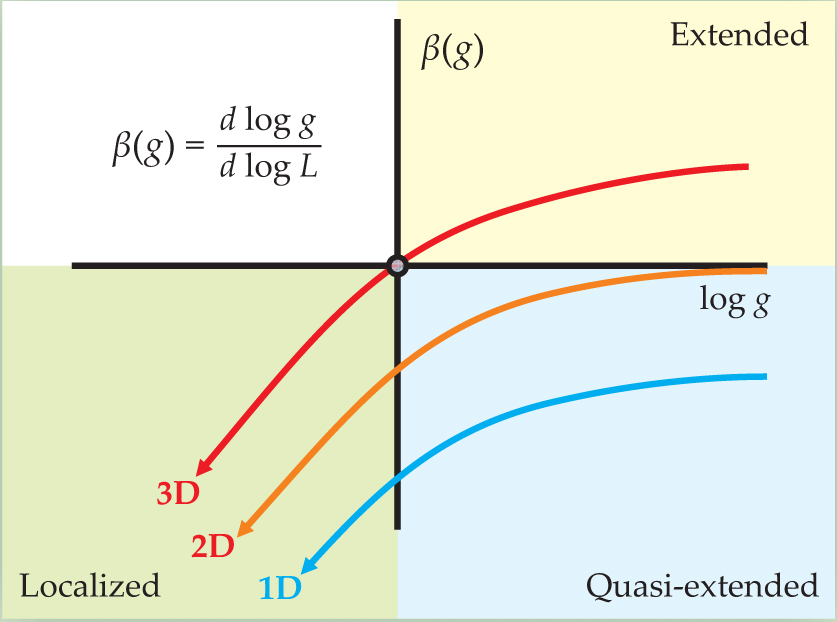
\includegraphics[width=1\textwidth]{beta_diagram.jpg}}
% \caption{Transition between ext. and loc. states is only possible in 3D. Taken from \cite{50yearsof}.}
% \end{figure}
% \end{minipage}
% \end{frame}

% \begin{frame}{The mobility edge}

% \begin{figure}
% \centering{
% 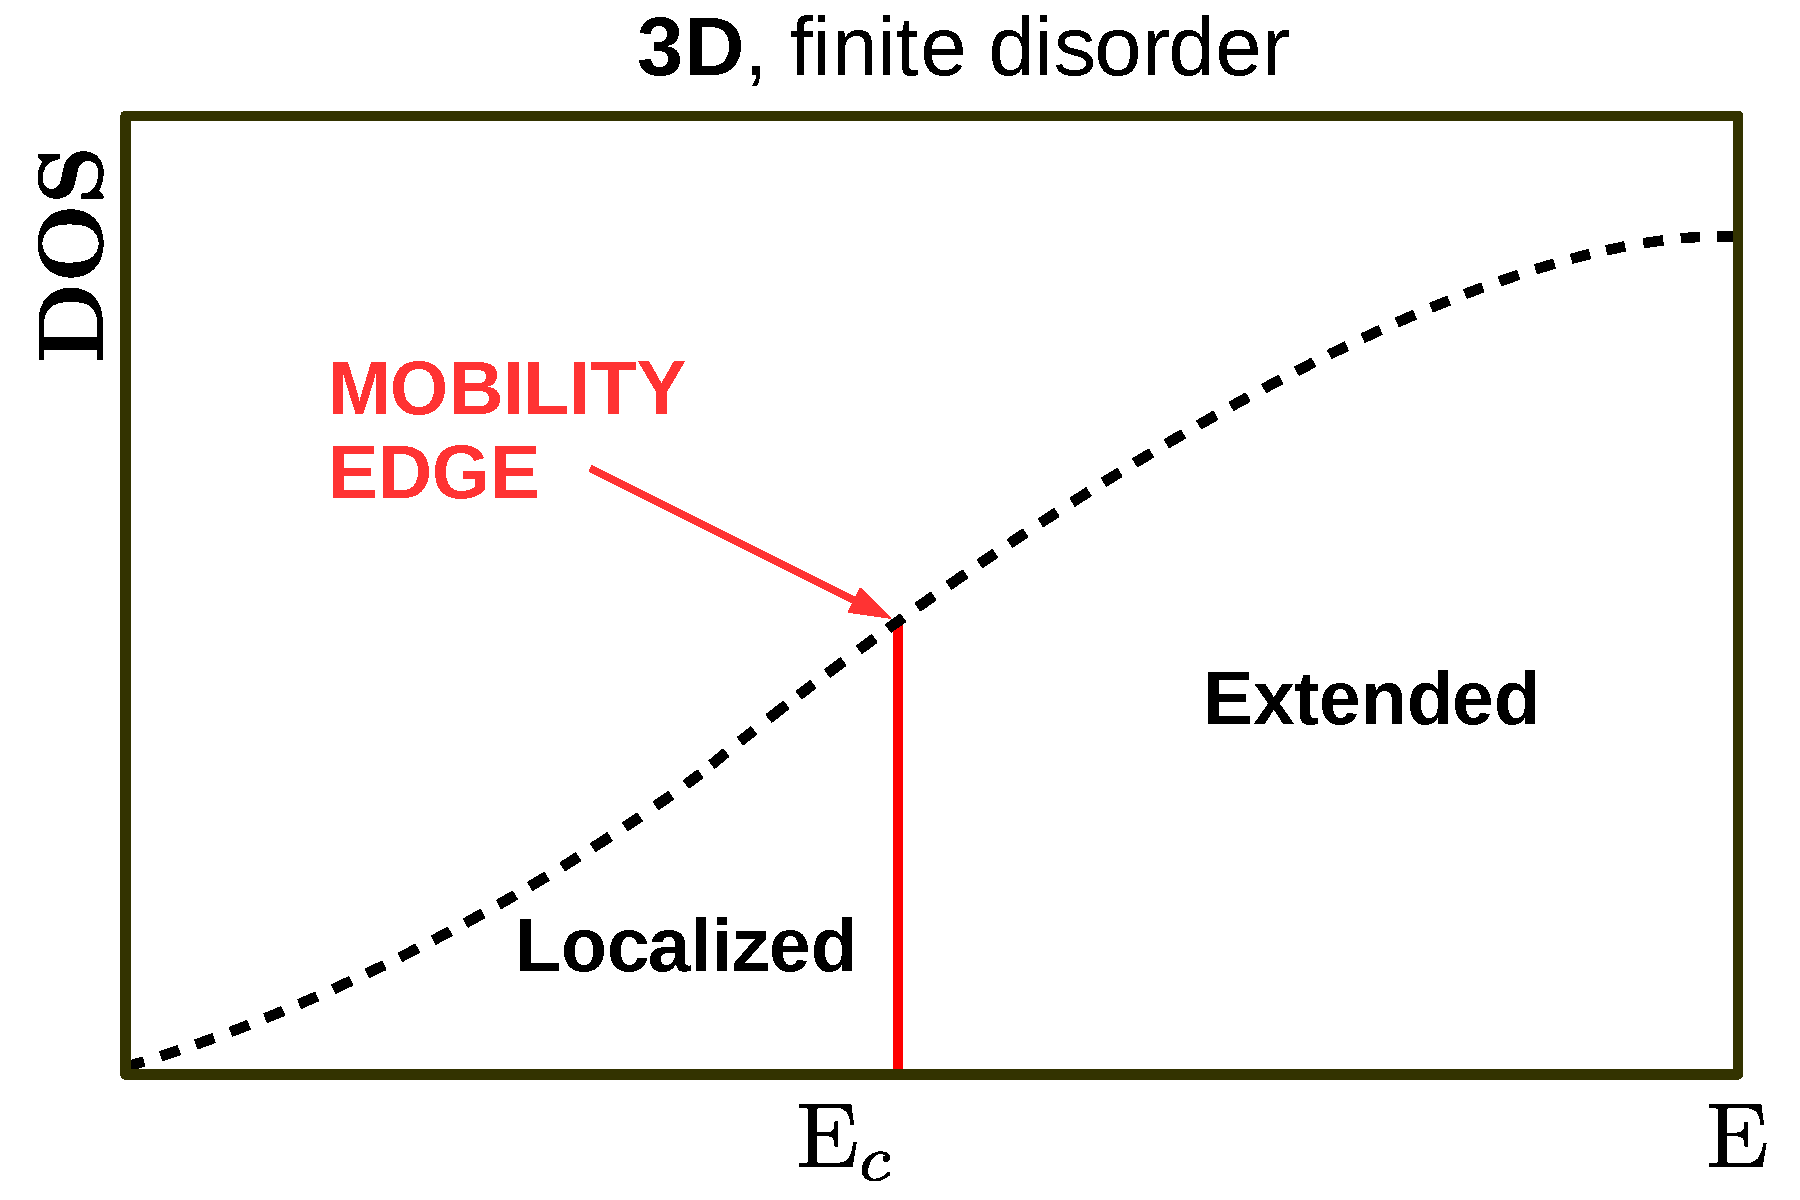
\includegraphics[width=1\textwidth]{mob_edge_schematic.pdf}}
% %\caption{Single-excitation dispersion relation}
% \end{figure}


% \end{frame}

% % \begin{frame}{The models of disorder}
% % \begin{minipage}[c]{0.57\textwidth}
% % \begin{itemize}
% % \item somehow distorting the \textbf{ideal crystal}\vspace{8mm}  
% % \end{itemize}
% % \begin{alertblock}{\centering\textbf{A generic Hamiltonian}}
% % $$
% % H=\frac{\hat{p}^2}{2m} + \sum\limits_{j=1}^N V_j(\mathbf{r}-\mathbf{R}_j)
% % $$
% % \end{alertblock}\vspace{10mm}
% % \begin{itemize}
% % \item we consider the \textbf{Anderson model}
% % \end{itemize}
% % \end{minipage}\hfill
% % \begin{minipage}[c]{0.4\textwidth}
% % \begin{figure}
% % \centering{
% % 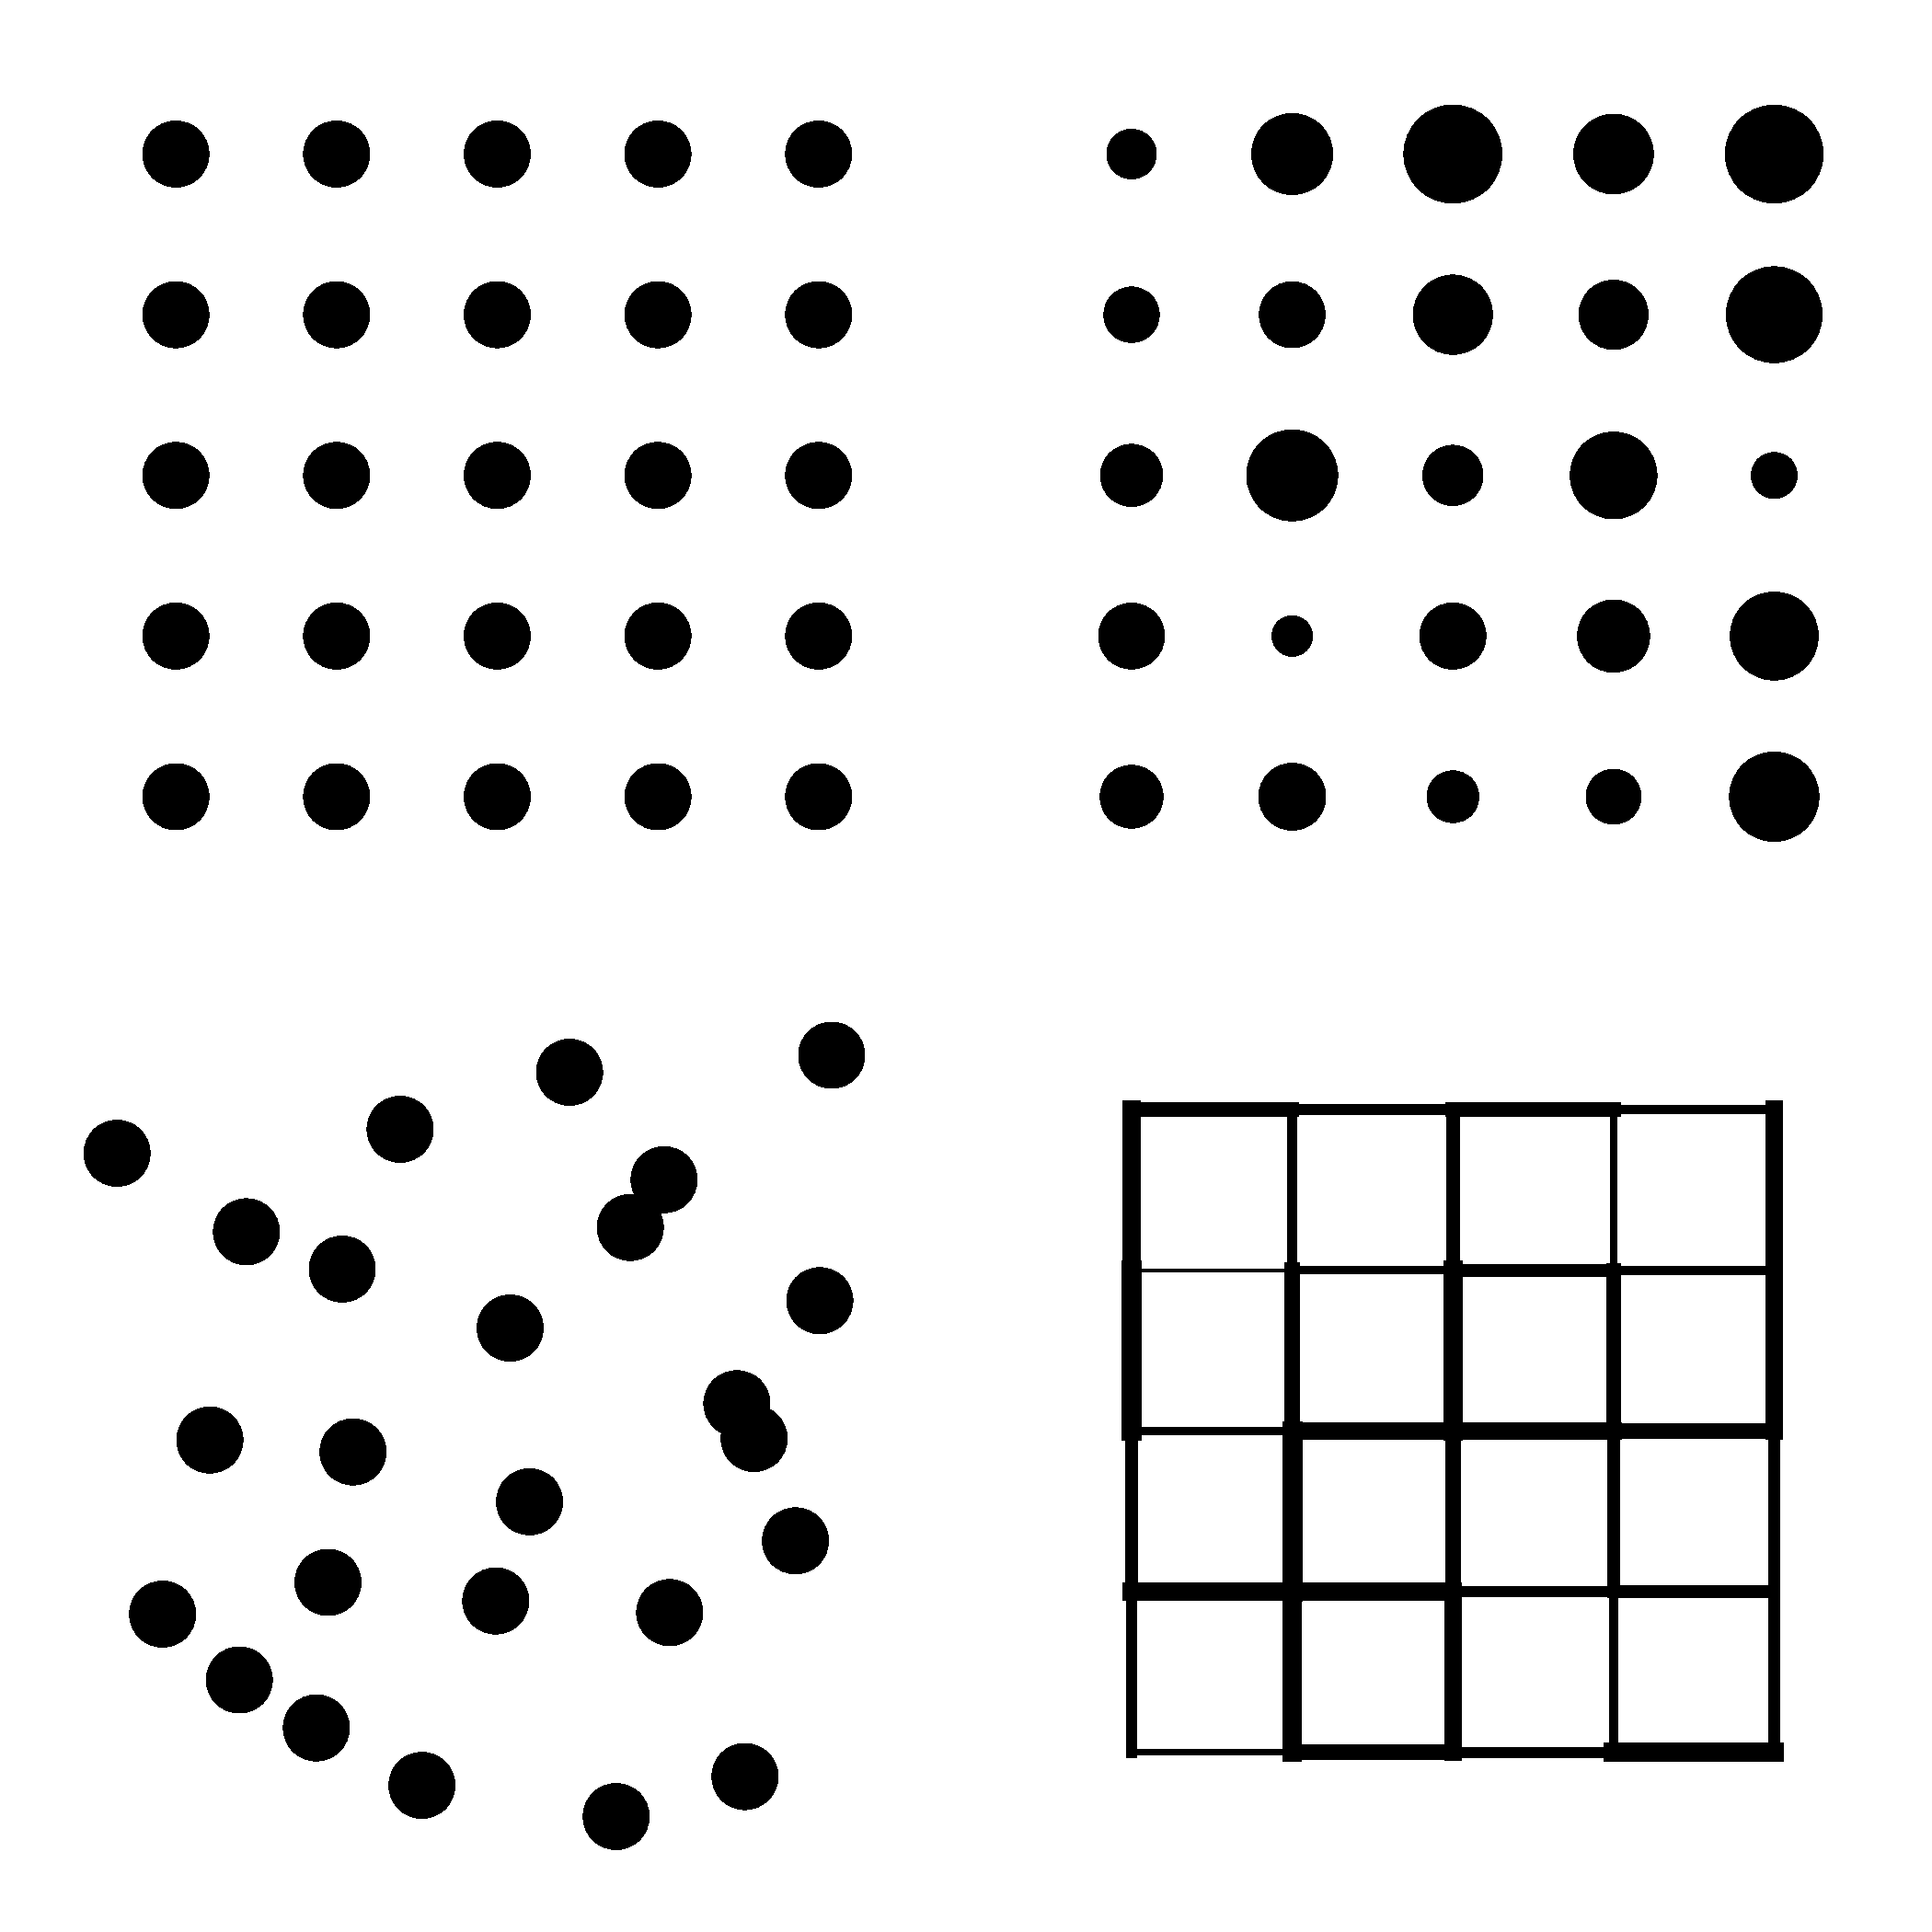
\includegraphics[width=1\textwidth]{disorder_scheme.pdf}}
% % \caption{Ideal crystal, compositional, structural and kinetic disorder. Adapted acc. to \cite{Kramer}.}
% % \end{figure}
% % \end{minipage}
% % \end{frame}

% \begin{frame}{Our model - the \textbf{Anderson model}}
% \begin{alertblock}{The Anderson Hamiltonian \cite{Anderson}}
% \begin{equation*}\label{eq:ising_hamiltonian}
% H=\sum\limits_j \varepsilon_j c^\dagger_jc_j - V\sum\limits_{\text{n.n.}} c^\dagger_{i}c_j + \text{h.c.}
% \end{equation*}
% \end{alertblock}{}
% \begin{minipage}[c]{0.48\textwidth}
% \begin{alertblock}{Probability distribution of $\varepsilon_j$}
% \begin{equation*}\label{eq:ising_hamiltonian}
% p(\varepsilon_j)=\frac{1}{2W}\Theta(W-|\varepsilon_j|)
% \end{equation*}
% \end{alertblock}{}
% \begin{figure}
% \centering{
% 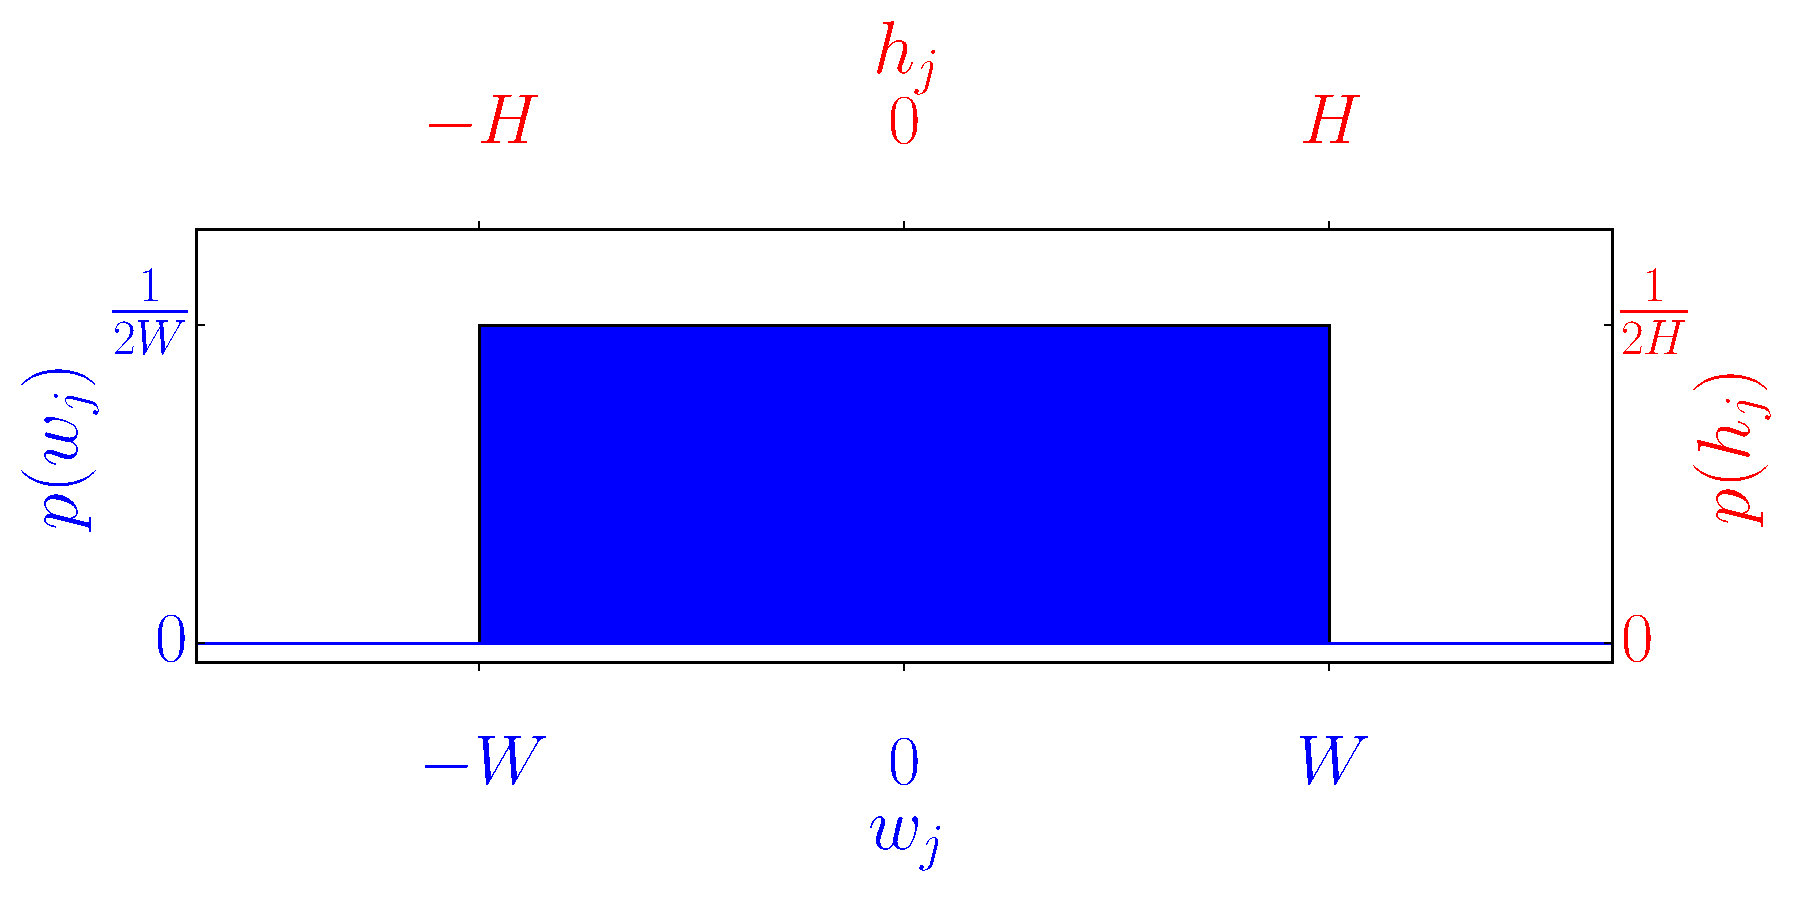
\includegraphics[width=1\textwidth]{prob_dist.pdf}}
% % \caption{The model in 2D.}
% \end{figure}
% \end{minipage}\hfill
% \begin{minipage}[c]{0.45\textwidth}
% \begin{figure}
% \centering{
% 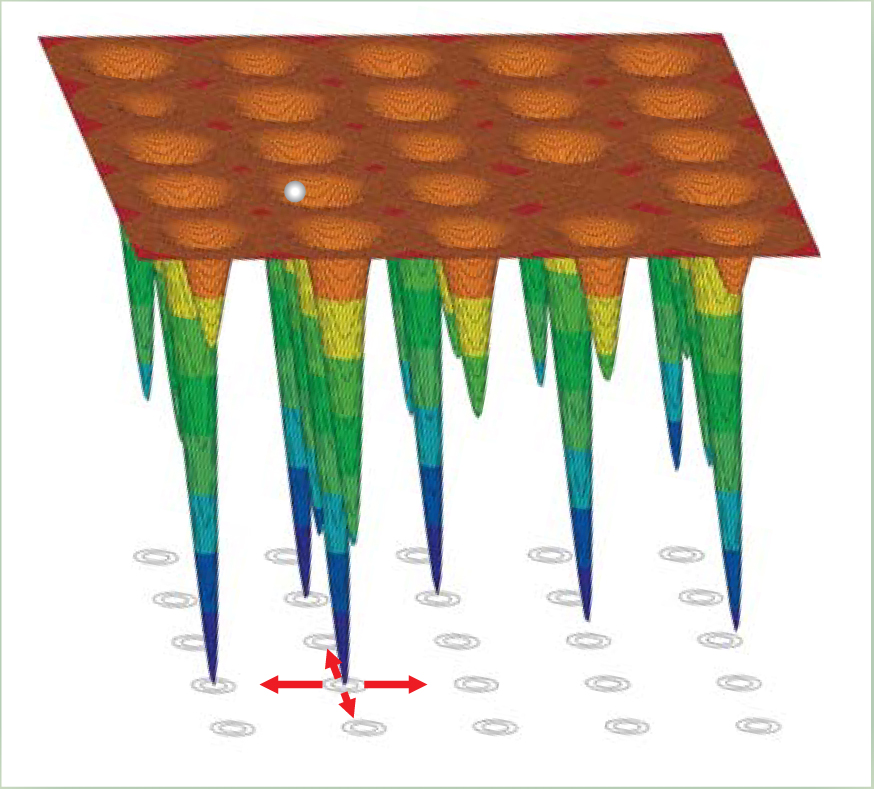
\includegraphics[width=1\textwidth]{hopping_picture_50years.jpg}}
% \caption{The model in 2D. Taken from \cite{50yearsof}.}
% \end{figure}
% \end{minipage}\hfill
% \end{frame}
% \begin{frame}{The Anderson model}

% % \begin{minipage}{0.38\textwidth}
% % \begin{figure}
% % \centering{
% % 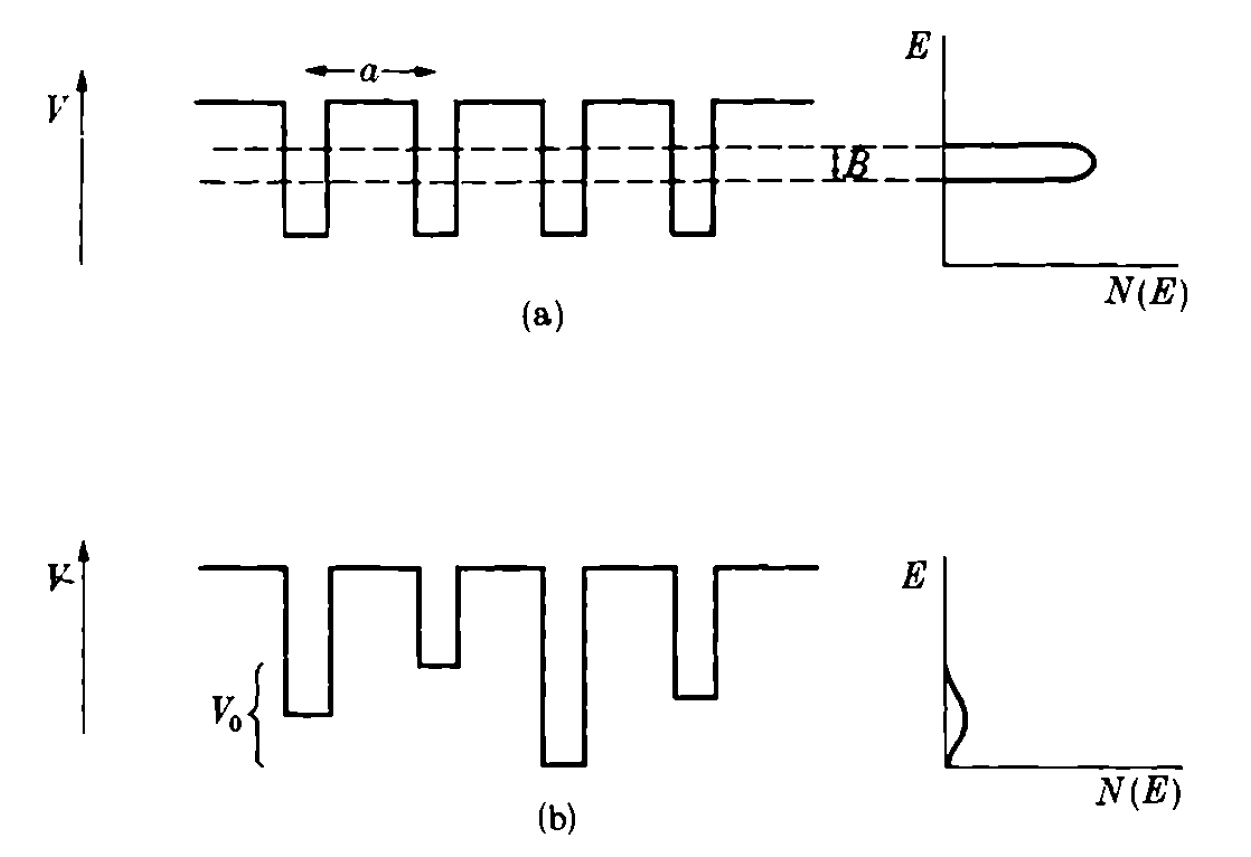
\includegraphics[width=1\textwidth]{bands.png}}
% % %\caption{Single-excitation dispersion relation}
% % \end{figure}
% % \end{minipage}\hfill\vspace{5mm}
% % \begin{minipage}{0.6\textwidth}
% % \begin{itemize}
% % 	\item Two mobility edges in 3D
% % \end{itemize}
% % \end{minipage}\\
% % \begin{minipage}{0.38\textwidth}
% % % Two mobility edges in 3D
% % \end{minipage}\hfill\vspace{5mm}
% % \begin{minipage}{0.7\textwidth}
% % \begin{figure}
% % \centering{
% % 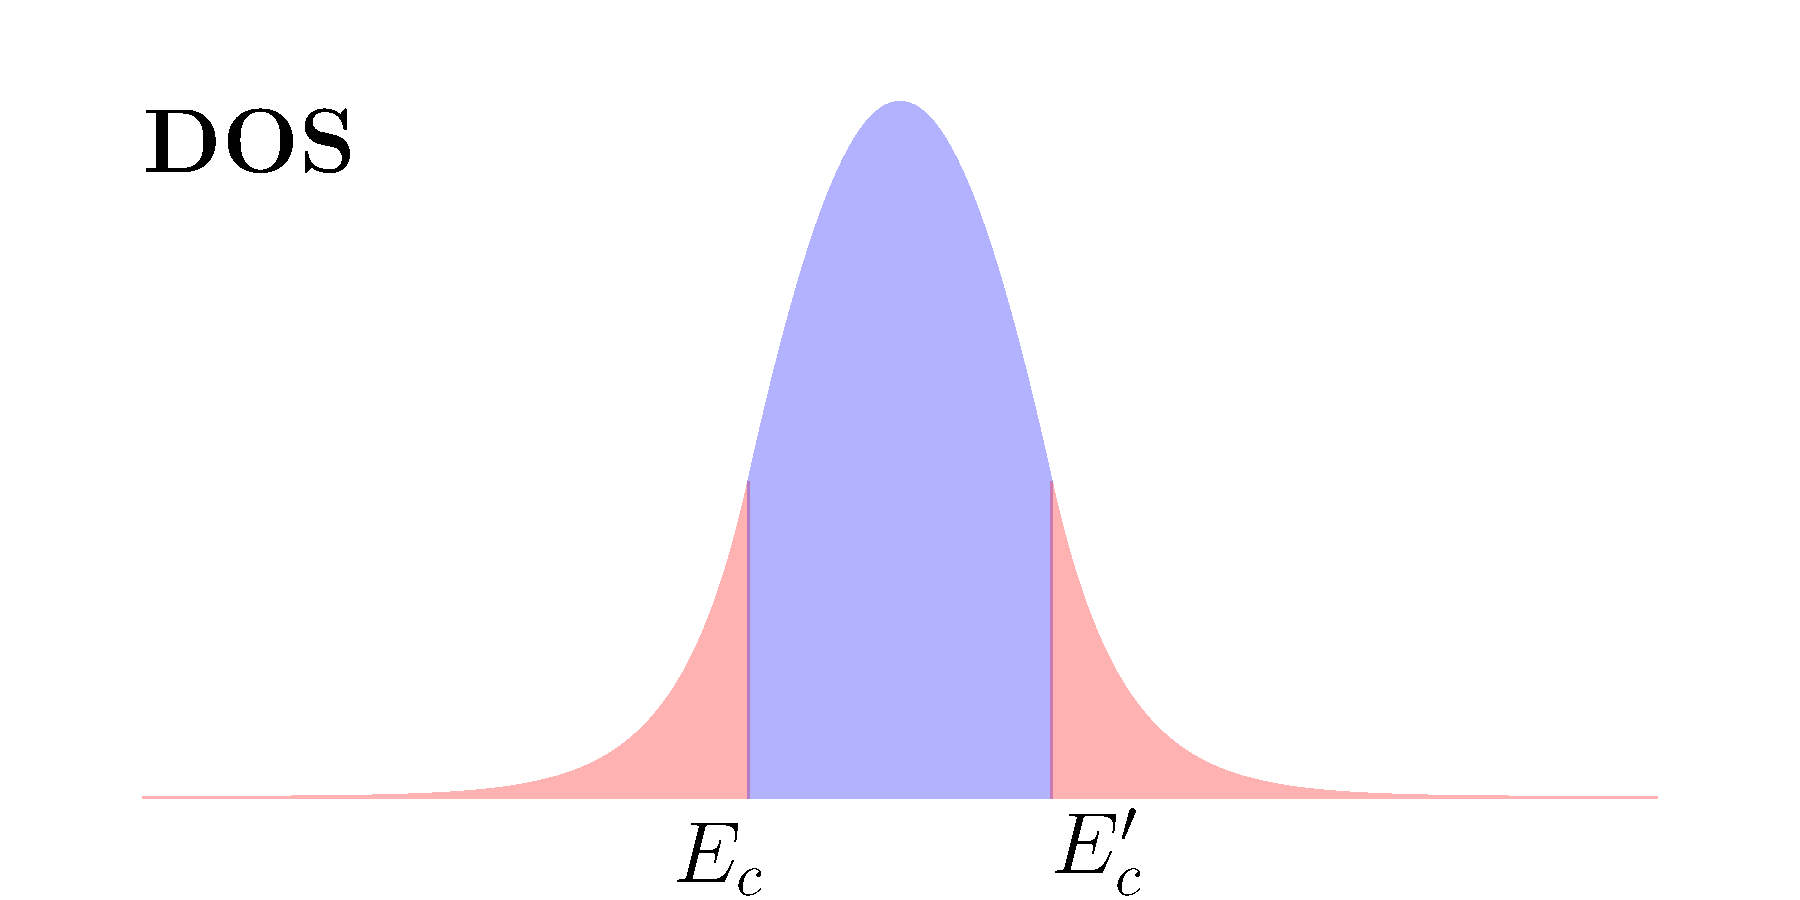
\includegraphics[width=1\textwidth]{mobility_edge_DOS.pdf}}
% % %\caption{The continuum splits into discrete states.}
% % \end{figure}
% % \end{minipage}

% \begin{itemize}
% 	\centering \item Two mobility edges in 3D
% \end{itemize}
% \begin{figure}
% \centering{
% 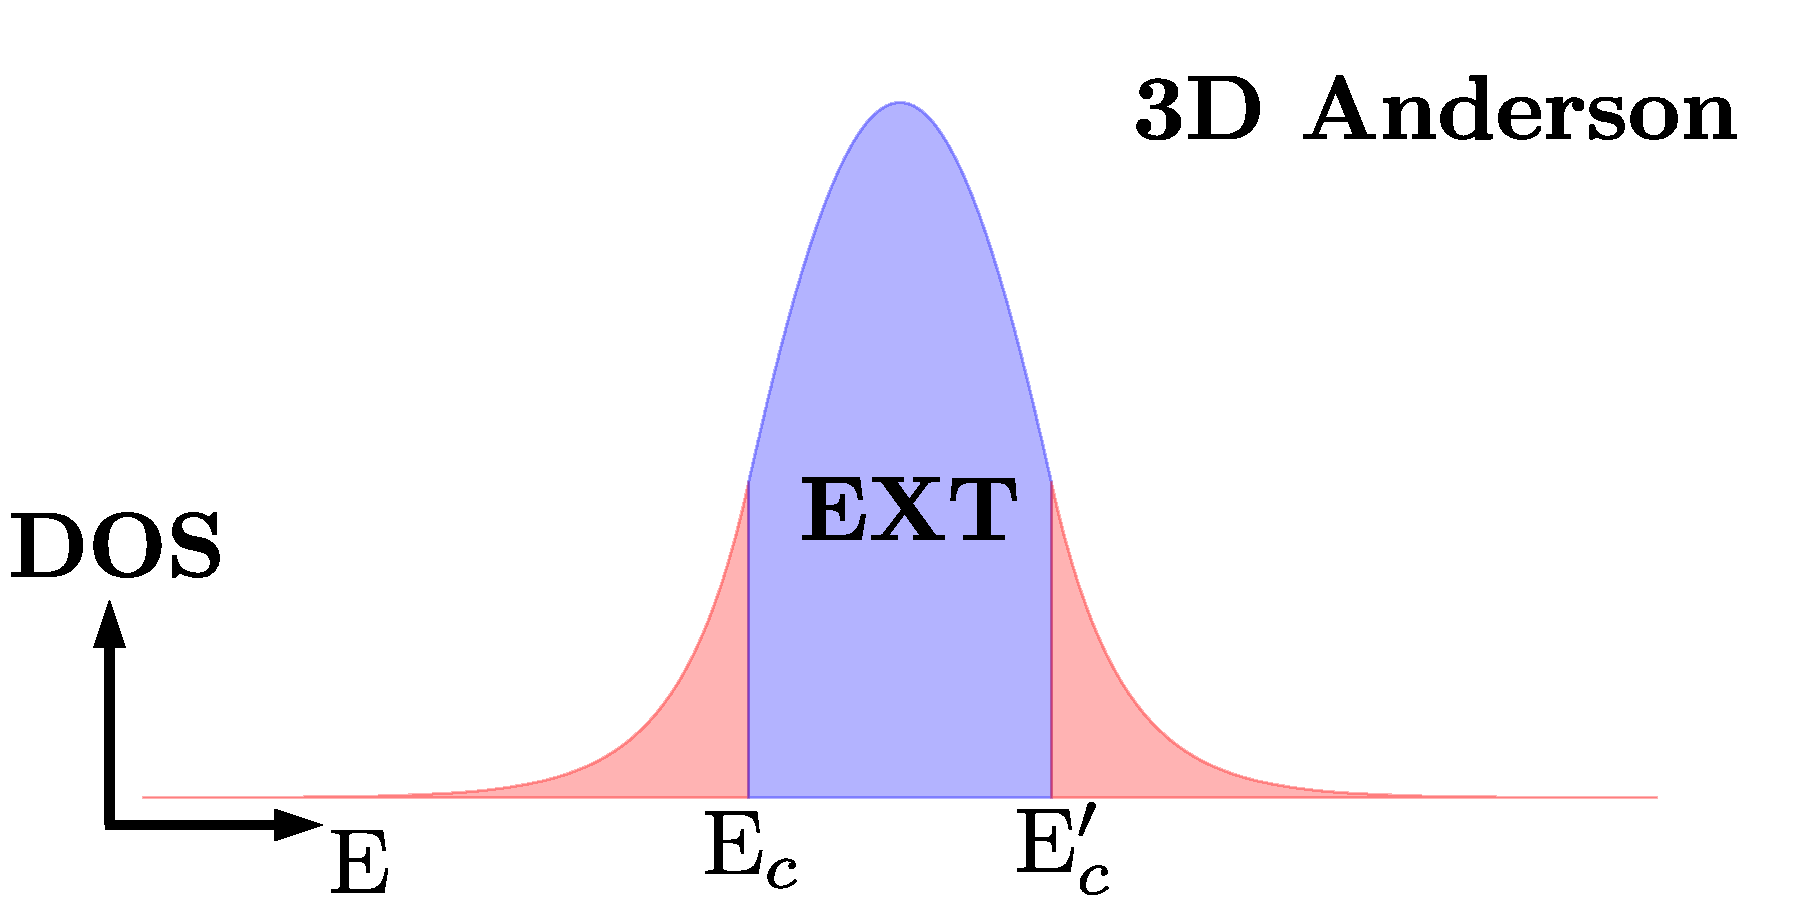
\includegraphics[width=1\textwidth]{mobility_edge_DOS_modified.pdf}}
% %\caption{The continuum splits into discrete states.}
% \end{figure}
% \end{frame}

% \begin{frame}{My work - the numerical simulations}
% \begin{itemize}
% \item How to extract features of the Anderson localization numerically?\vspace{5mm}
%  \begin{itemize}
% 	\item implementation in 1D, 2D and 3D \vspace{2mm}
% 	\item calculations were run at the F-1 cluster at IJS \vspace{2mm}
% 	\item Full diagonalization and time evolution calculations
% \end{itemize}\vspace{5mm}
% \item Two localization criteria: \vspace{5mm}
% \begin{itemize}
% 	\item the \textbf{inverse participation ratio} (IPR)\vspace{2mm}
% 	\item the \textbf{absence of diffusion}
% \end{itemize}
% \end{itemize}
% \end{frame}

% \begin{frame}{Localization criteria - the IPR}
% \begin{alertblock}{The definition}
% \begin{equation*}
% P^{-1}=\sum\limits_\mathbf{r} |\psi(\textbf{r})|^4, \hspace{5mm} \norm{\psi}=1.
% \end{equation*}
% \end{alertblock}{}\vspace{5mm}
% \begin{itemize}
% 	\item sum over the lattice sites
% 	\end{itemize}\vspace{5mm}
% \begin{alertblock}{\centering{If $L$ large enough}}
% $$
% P^{-1} \propto\begin{cases}
% &1/L^d, \hspace{5mm} \text{extended} \\
% &\text{const}, \hspace{5mm} \text{localized} 
% \end{cases}
% $$ 
% % smaller for extended states, larger for extended ones \vspace{10mm}
% % \item Full Hamiltonian diagonalization needed 
% \end{alertblock}{}
% % \begin{figure}
% % \centering{
% % 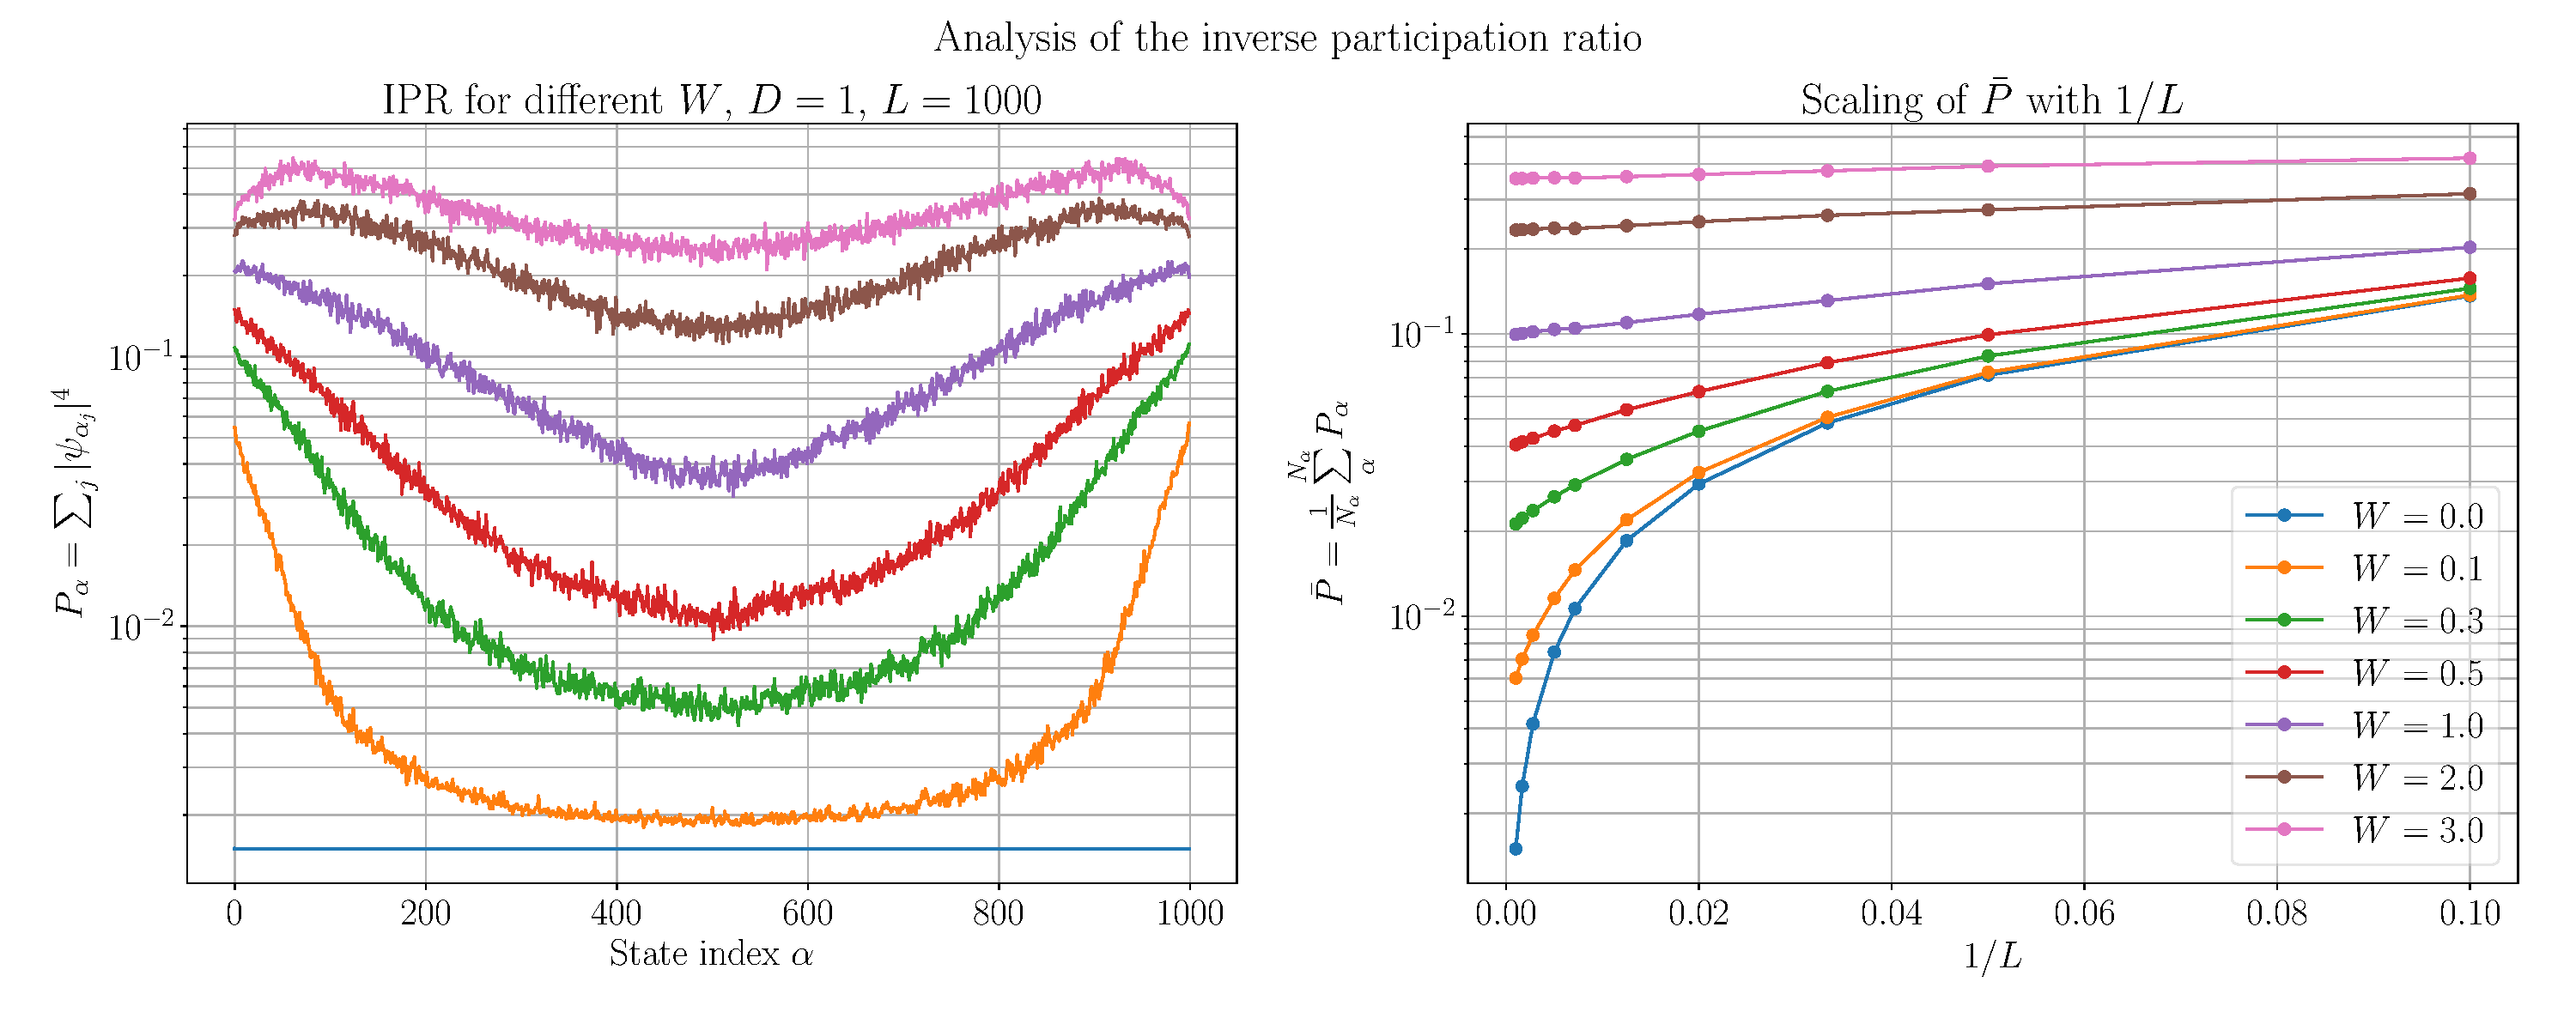
\includegraphics[width=1\textwidth]{1D_Anderson_localization_Seminar_scaling_analysis_D1_shape_1000_ipr_plots.pdf}}
% % %\caption{The continuum splits into discrete states.}
% % \end{figure}
% \end{frame}

% \begin{frame}{IPR - the results}
% \begin{figure}
% \centering{
% 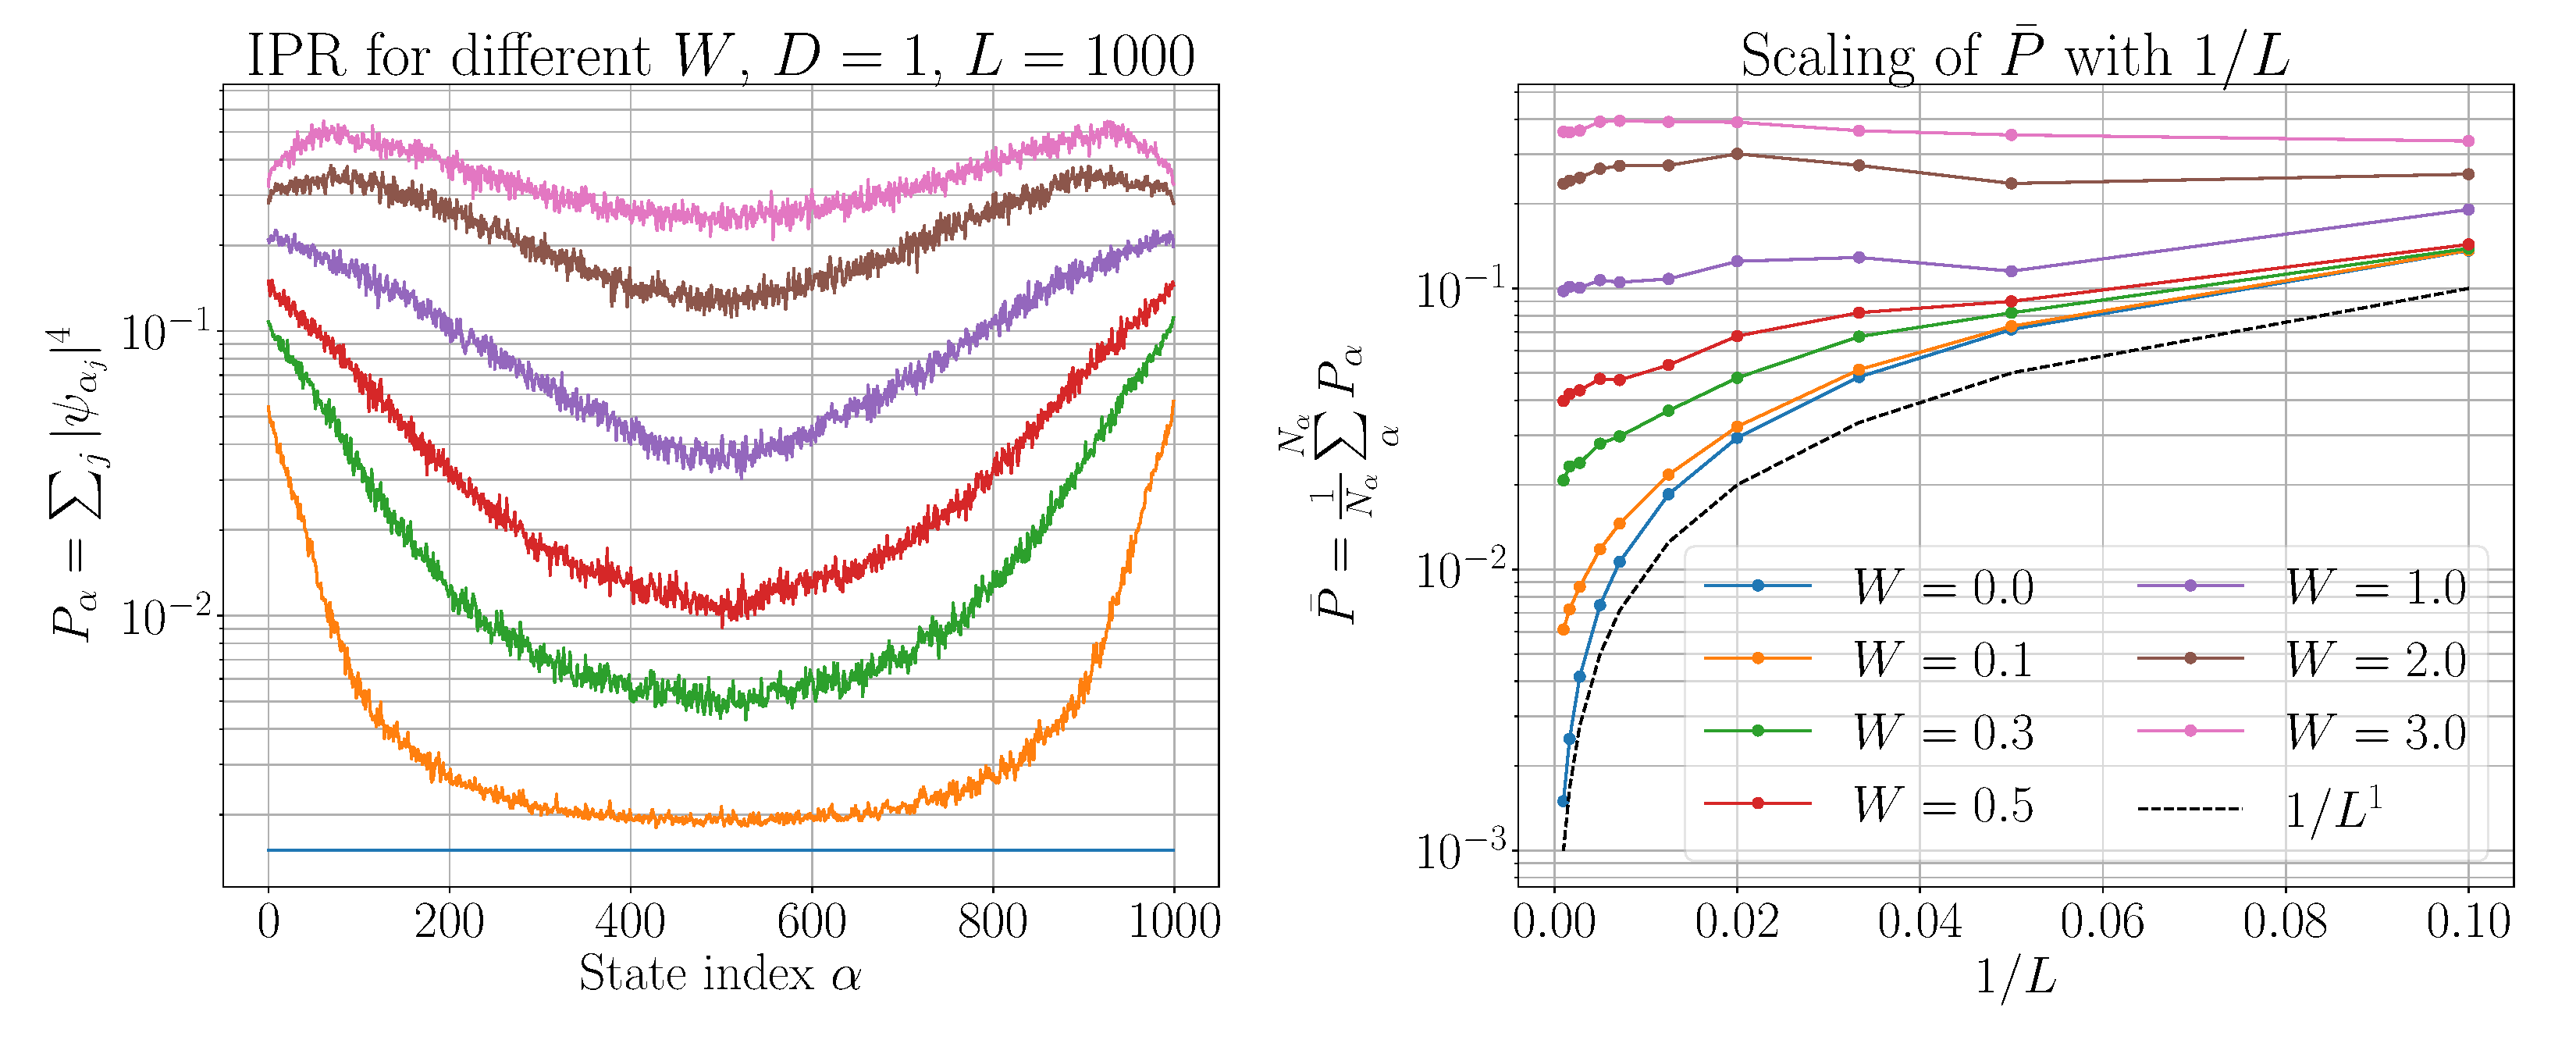
\includegraphics[width=0.75\textwidth]{1D_Anderson_localization_Seminar_scaling_analysis_D1_shape_1000_ipr_plots_presentation.pdf}}
% %\caption{The continuum splits into discrete states.}
% \end{figure}
% \begin{figure}
% \centering{
% 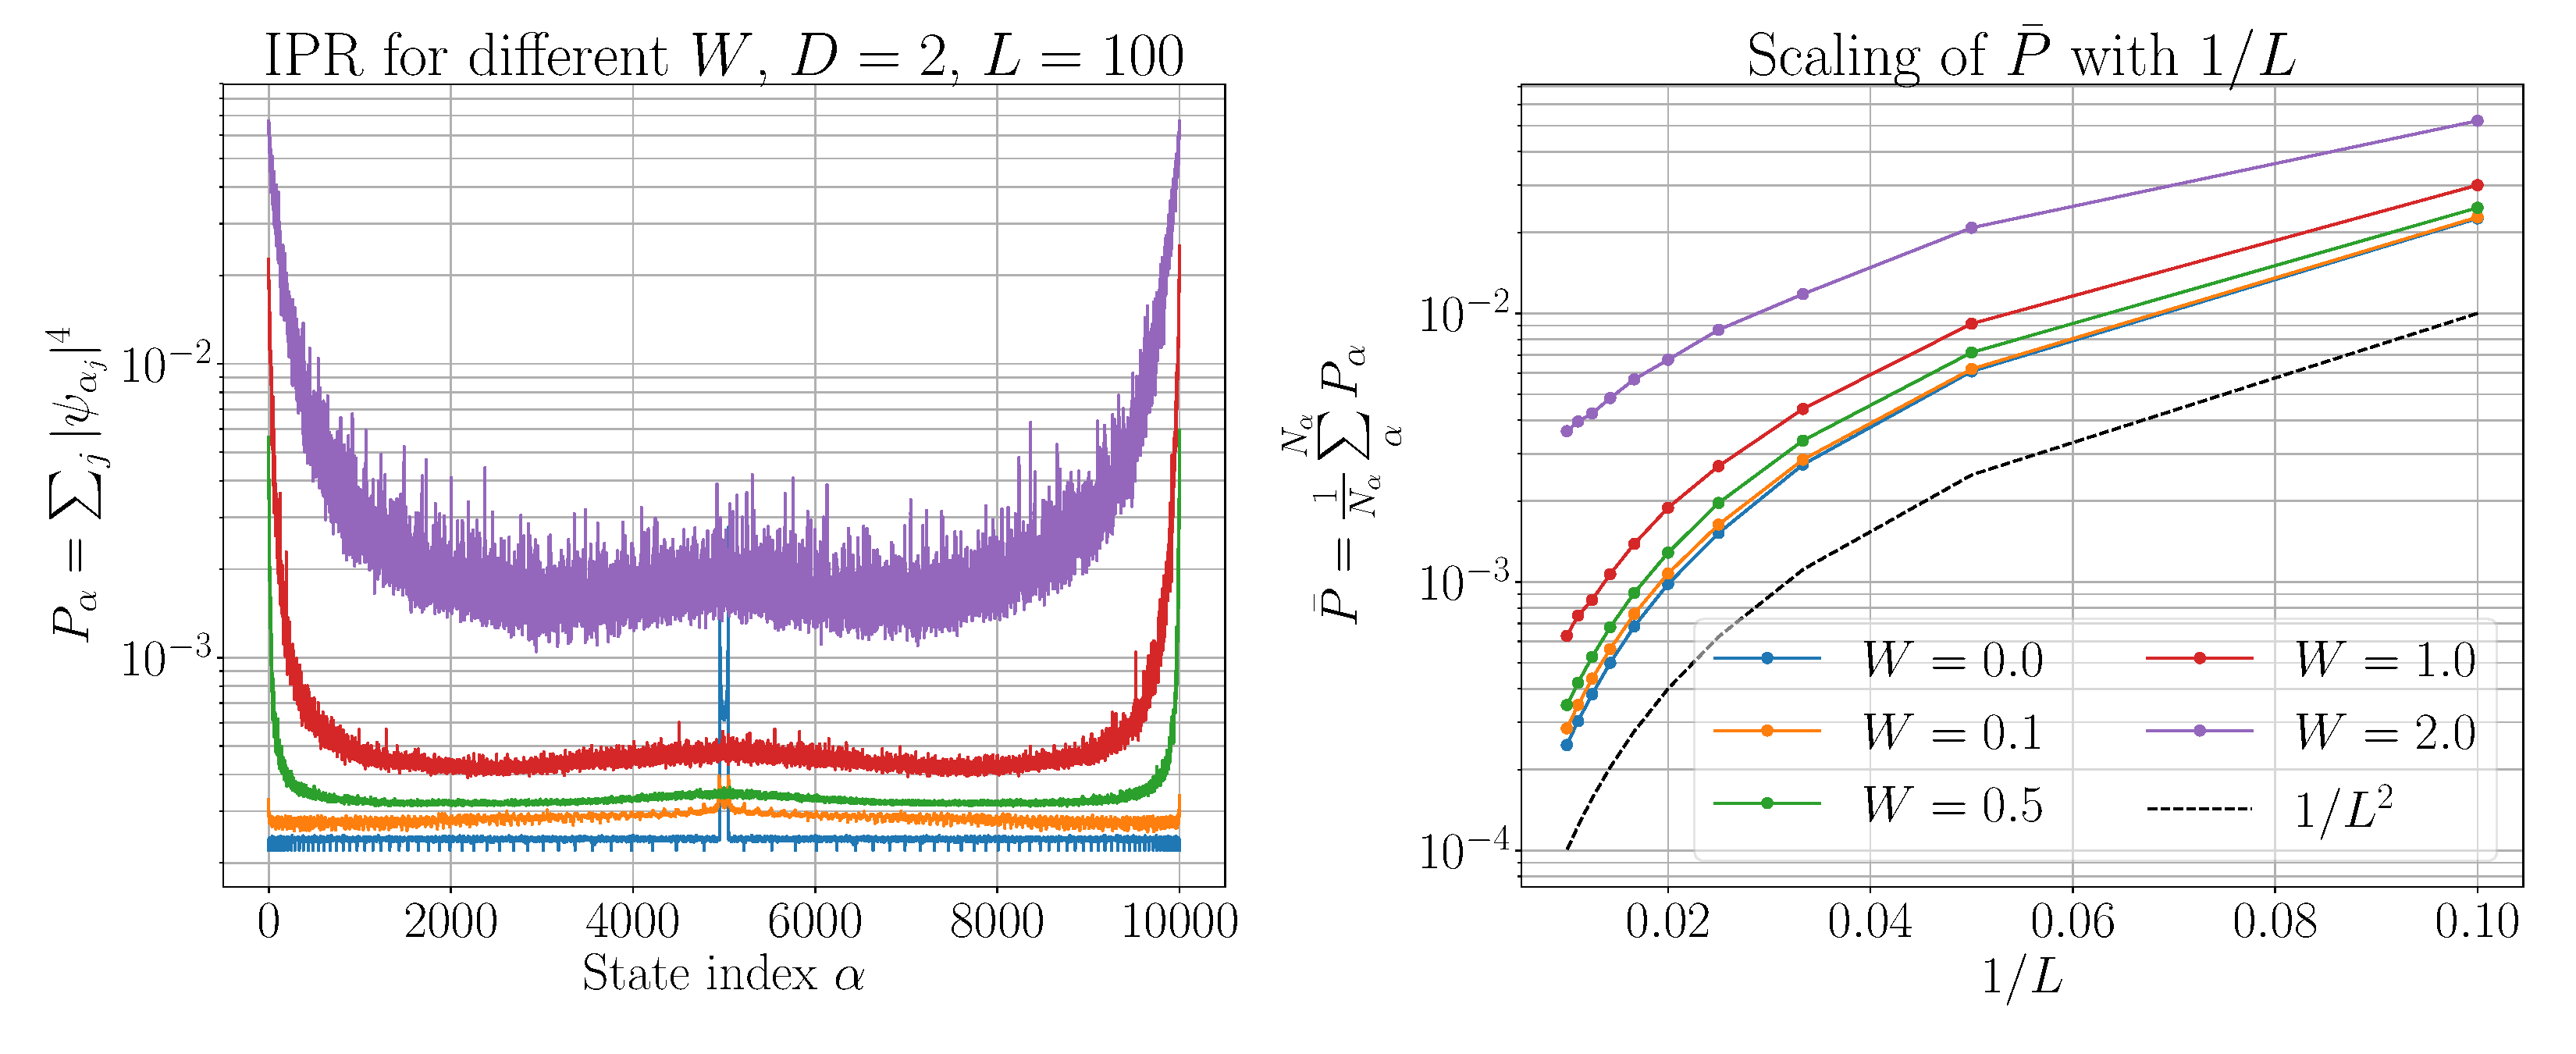
\includegraphics[width=0.75\textwidth]{2D_Anderson_localization_Seminar_scaling_analysis_D2_shape_100_100_ipr_plots_presentation.pdf}}
% %\caption{The continuum splits into discrete states.}
% \end{figure}
% \end{frame}

% \begin{frame}{IPR 3D}
% \begin{figure}
% \centering{
% 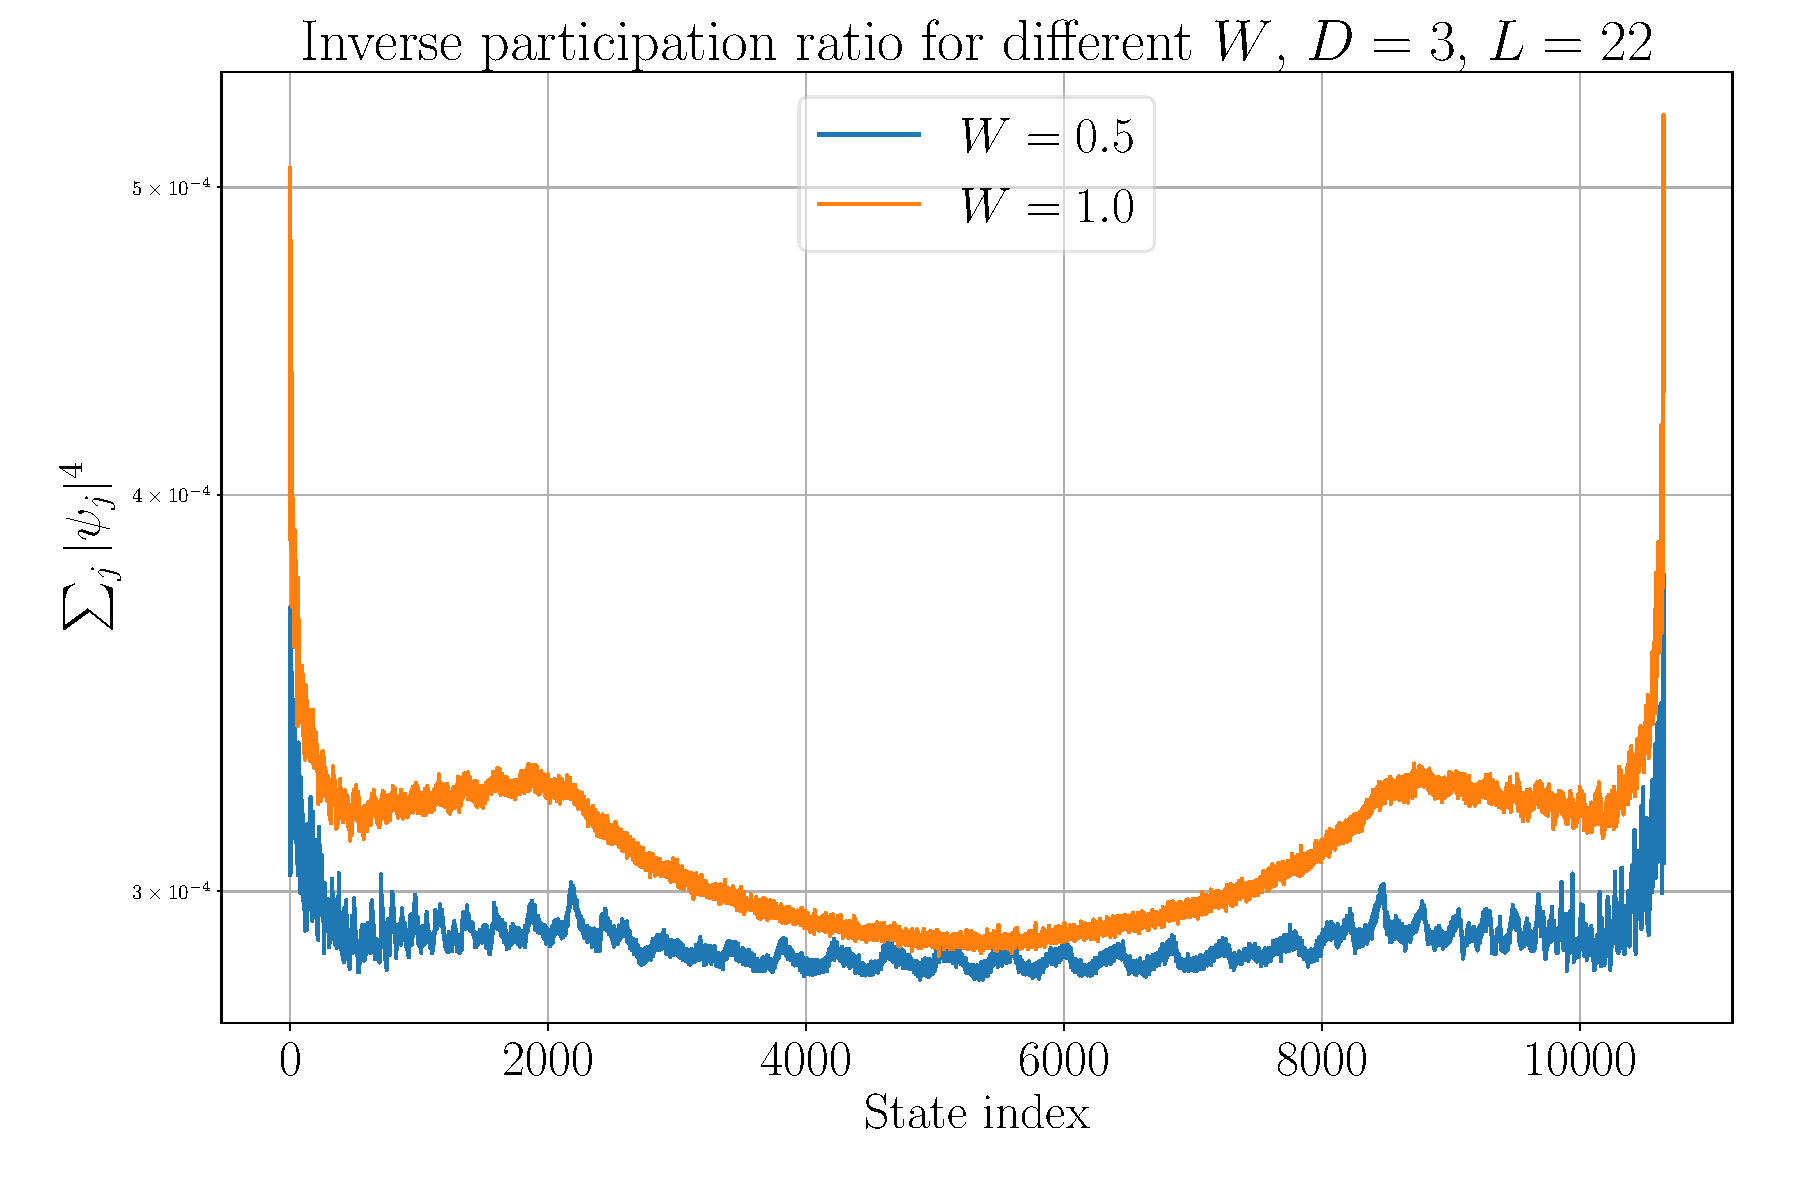
\includegraphics[width=0.9\textwidth]{3D_Anderson_localization_Seminar_scaling_analysis_D3_shape_22_22_22_eigensys_plots_single_presentation_nozero.pdf}}
% %\caption{The continuum splits into discrete states.}
% \end{figure}
% \end{frame}

% \begin{frame}{Absence of diffusion}
% \begin{alertblock}{Time evolution}
% \begin{equation*}
% \ket{\psi, t+\mathrm{d}t}=\exp\left(-\mathrm{i}\hat{H}\dd t\right)\ket{\psi, t},
% \end{equation*}
% \end{alertblock}{}\vspace{2mm}
% \begin{minipage}{0.28\textwidth}
% \begin{alertblock}{}
% $$
% \hat{R^2}=\sum\limits_{\mathbf{r}_j} \mathbf{r}_j^2 \hat{n}_{\mathbf{r}_j}, 
% $$
% \end{alertblock}{}
% \begin{alertblock}{}
% $$
% \beta(t)=\frac{\dd \log R}{\dd \log t}
% $$
% \end{alertblock}{}
% \end{minipage}\hfill
%  \begin{minipage}{0.7\textwidth}
% \begin{figure}
% \centering{
% 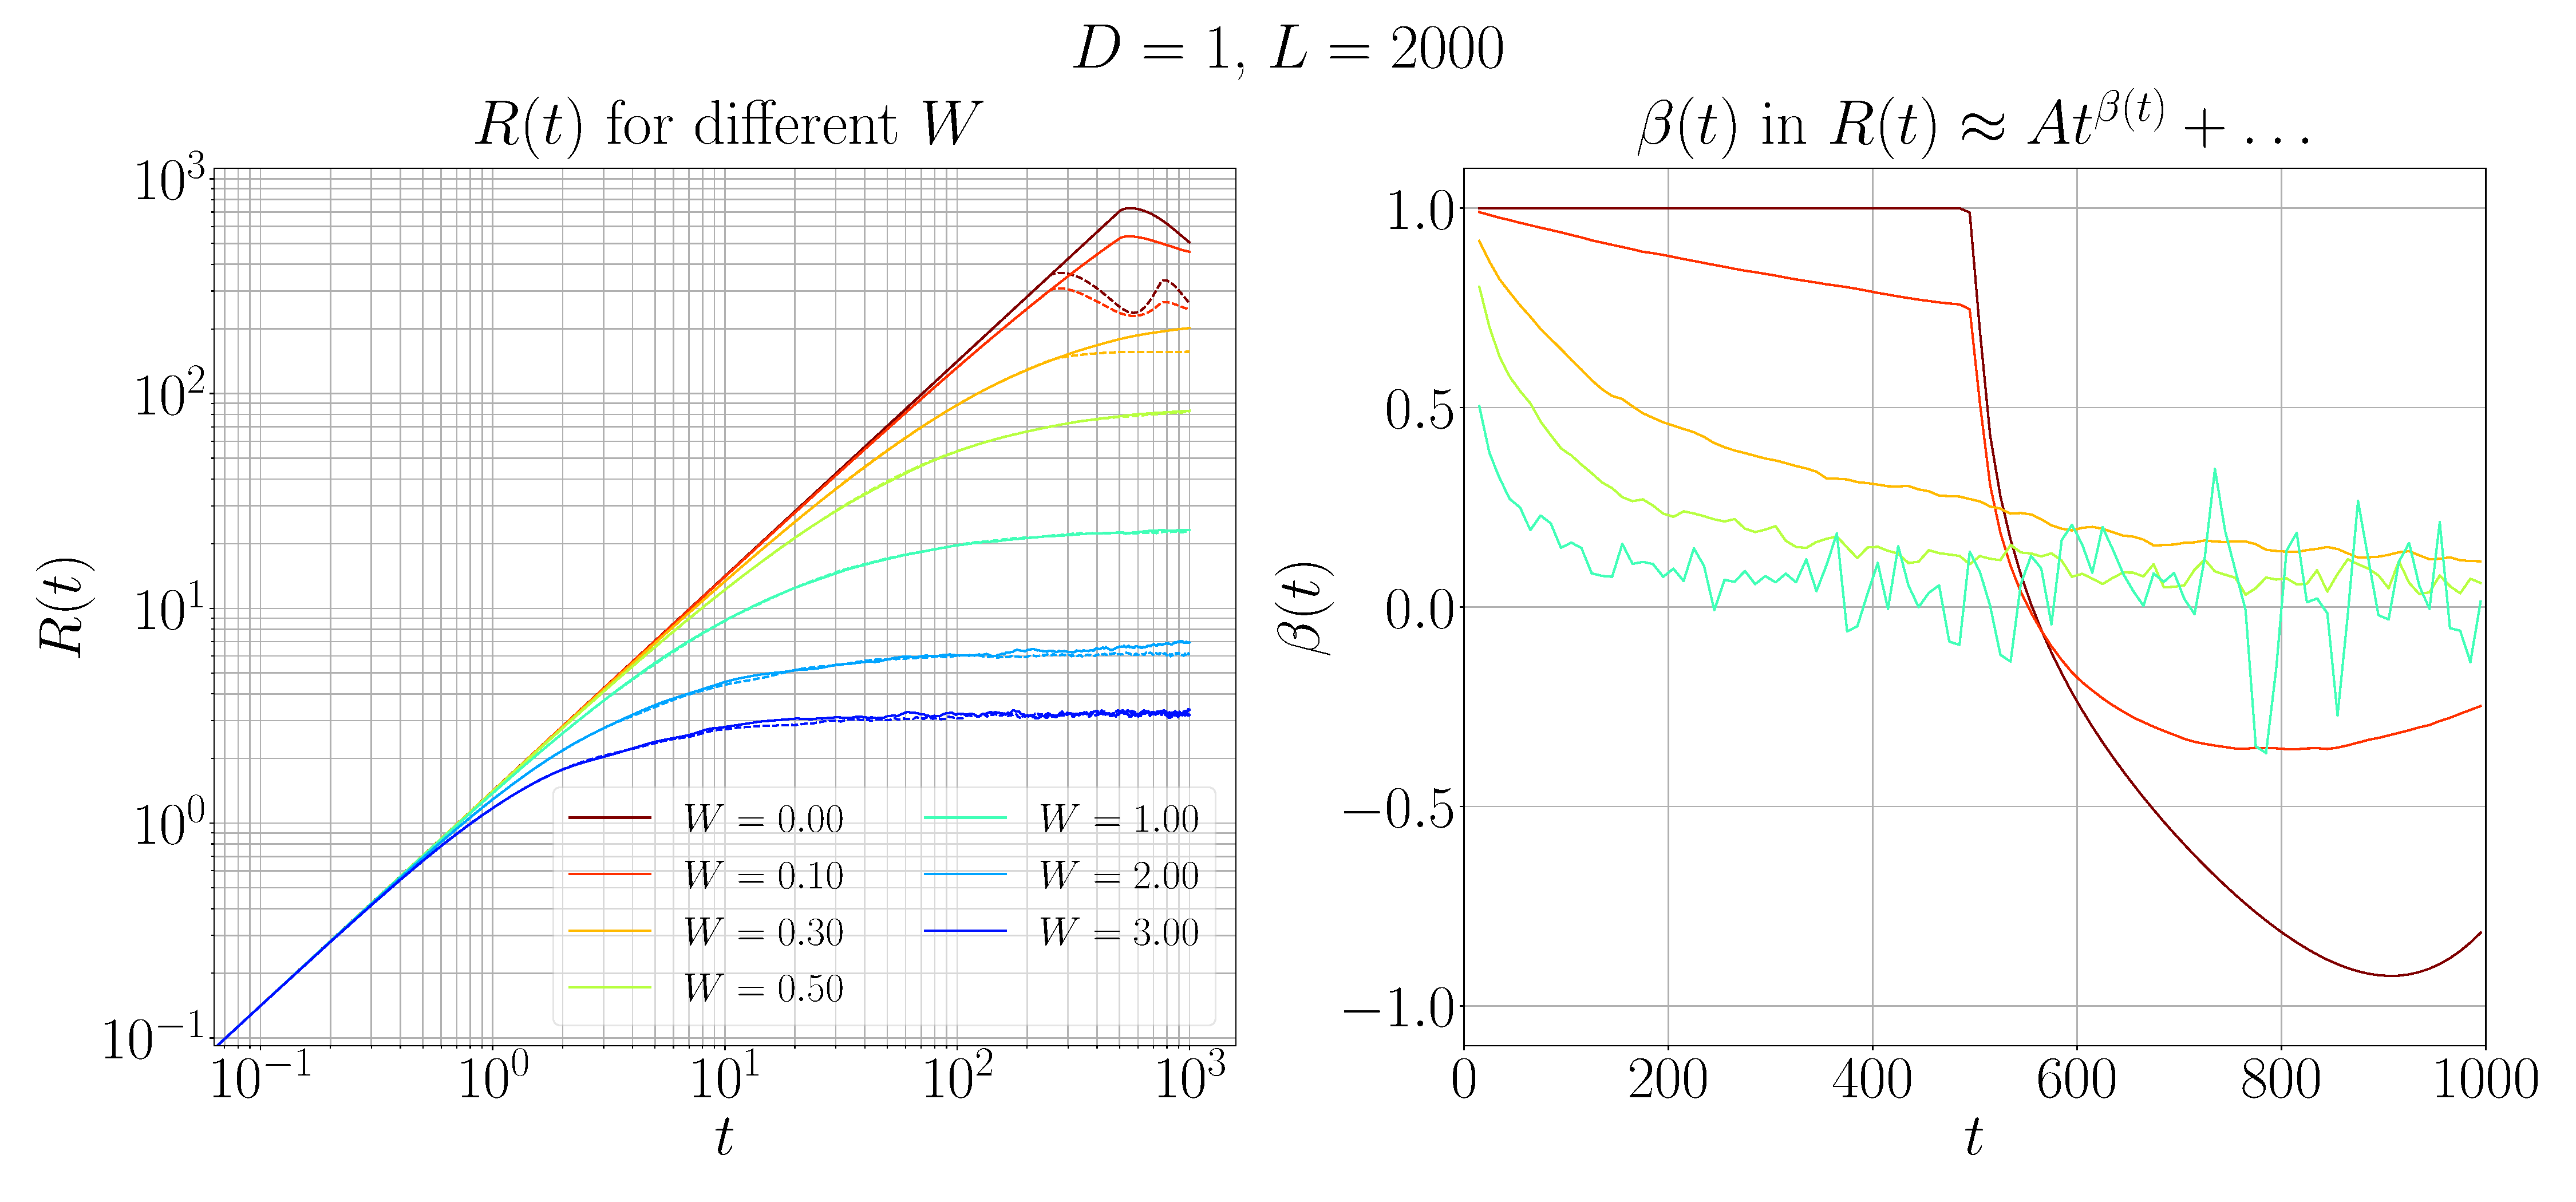
\includegraphics[width=1\textwidth]{1D_Anderson_localization_Seminar_scaling_analysis_D1_shape_2000_r_sq_dynamics_presentation.pdf}}
% %\caption{Single-excitation dispersion relation}
% \end{figure}
% \end{minipage}
% \begin{alertblock}{}
% $$
% R(t)=\sqrt{\bra{\psi,t} \hat{R^2}\ket{\psi,t}-\bra{\psi,0} \hat{R^2}\ket{\psi,0}} 
% $$
% \end{alertblock}{}
% \end{frame}

% \begin{frame}{Absence of diffusion, 2D}
% \begin{figure}
% \centering{
% 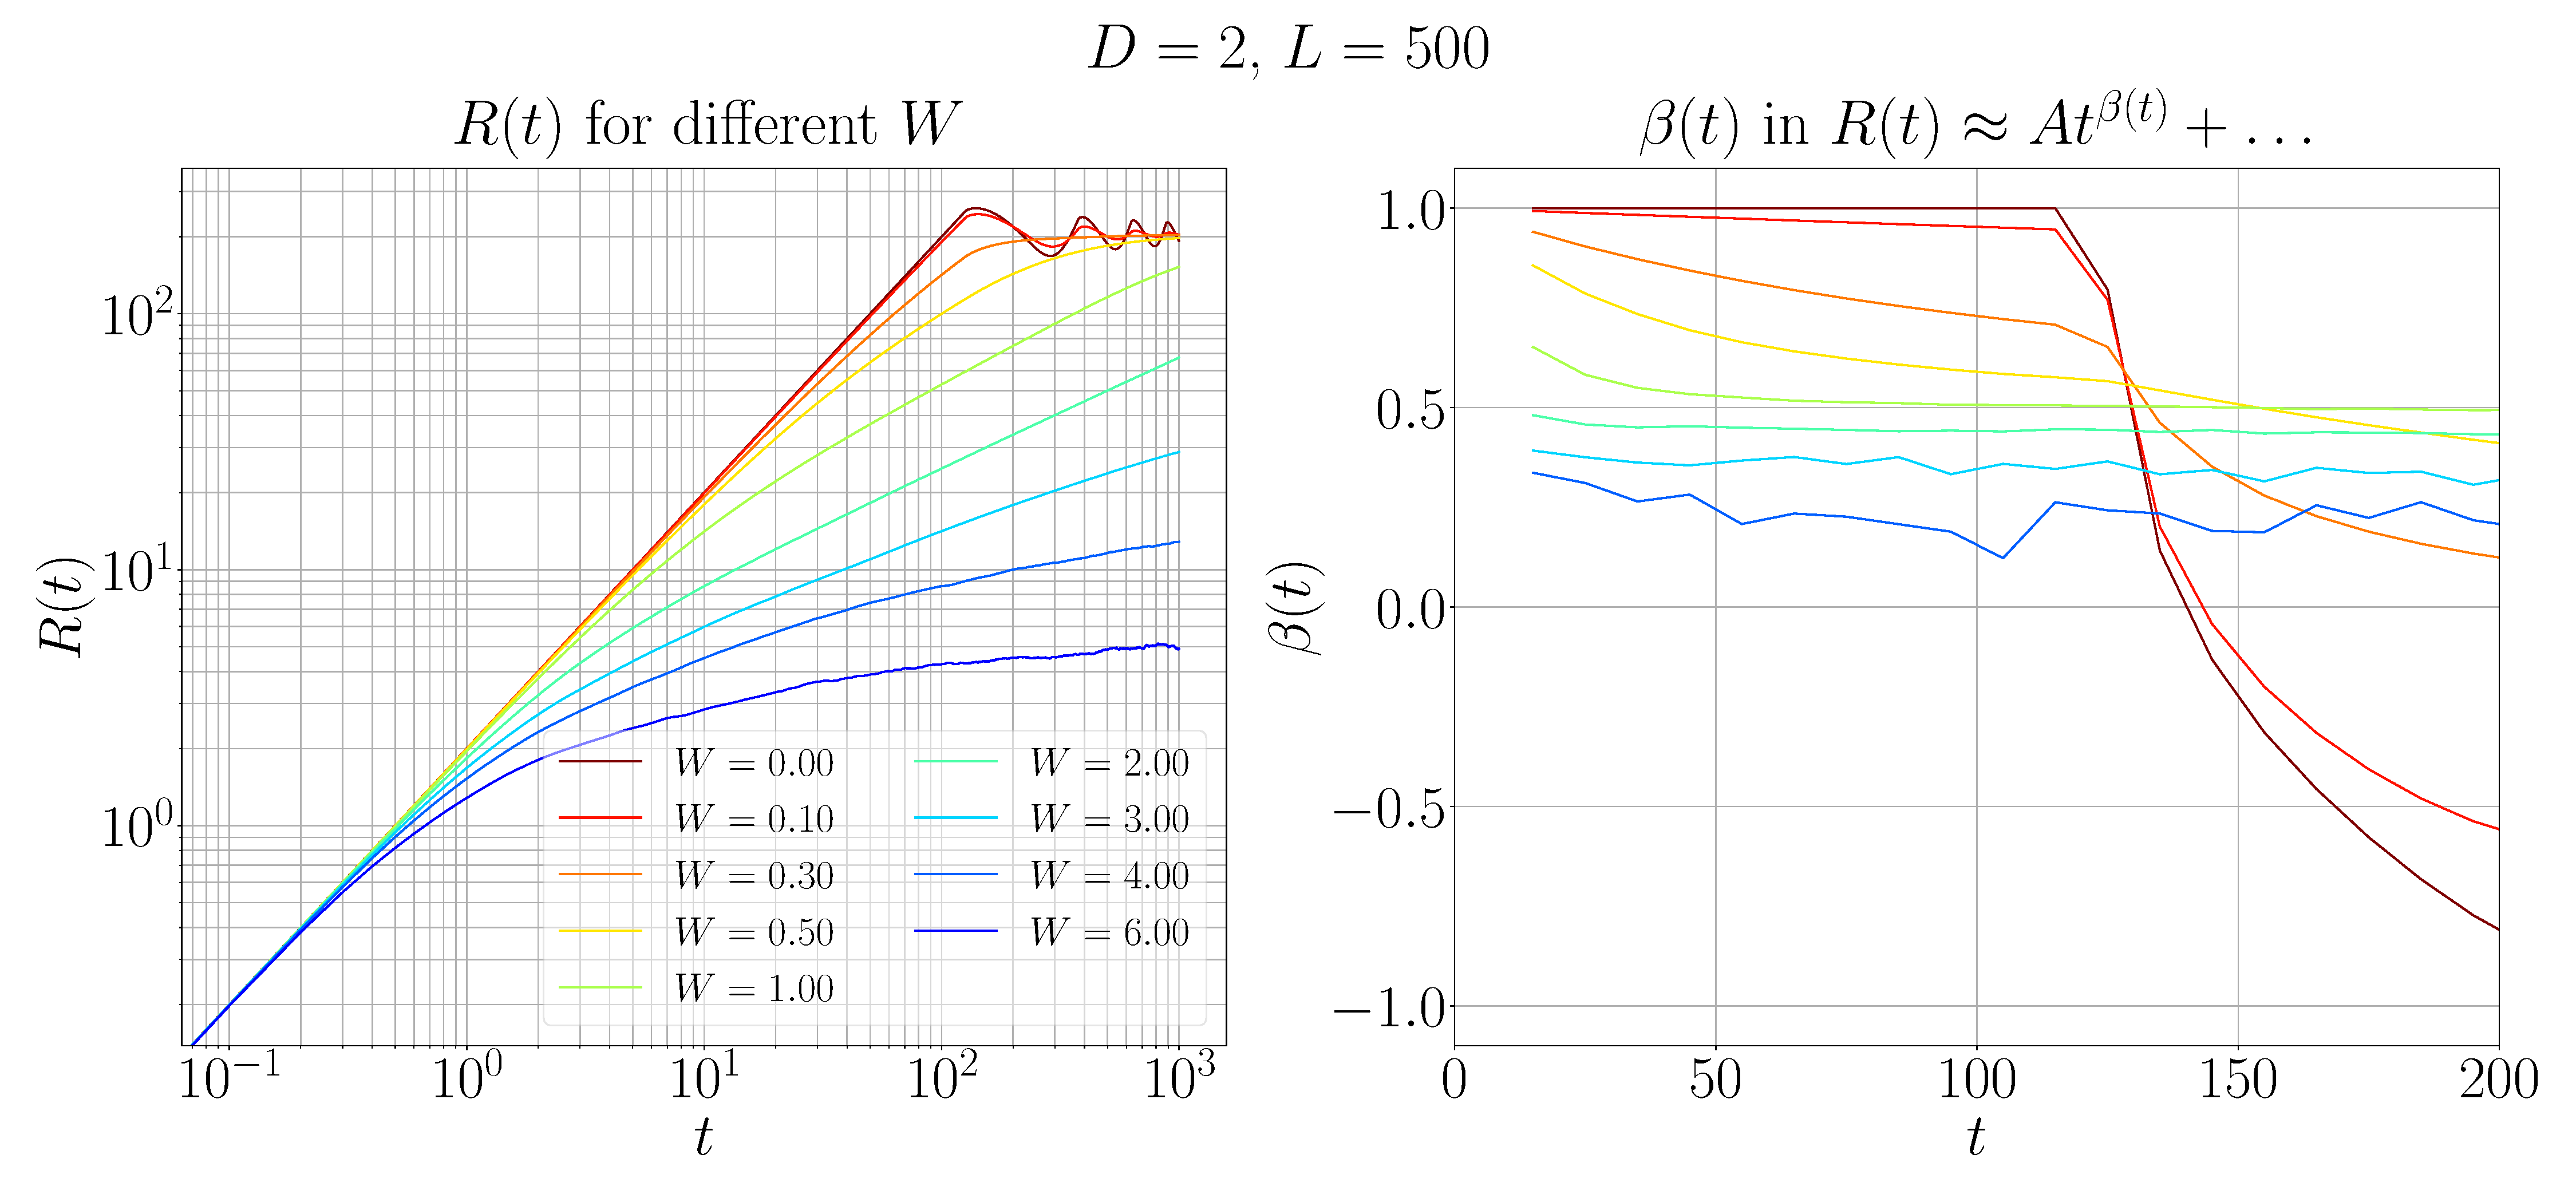
\includegraphics[width=1\textwidth]{2D_Anderson_localization_Seminar_scaling_analysis_D2_shape_500_500_r_sq_dynamics_presentation.pdf}}
% %\caption{Single-excitation dispersion relation}
% \end{figure}

% \end{frame}

% \begin{frame}{Many-body localization}
% \only<1->{\begin{alertblock}{\centering What happens when \textbf{INTERACTIONS} are included?}
% \end{alertblock}} 
% \onslide<2->{
% \begin{minipage}{0.28\textwidth}
% \begin{itemize}
% \item Localization for low T, weak interactions
% \end{itemize}
% \end{minipage}\hfill
% \begin{minipage}{0.60\textwidth}
% \begin{figure}
% \centering{
% \includegraphics[width=0.94\textwidth]<2->{excerpt_basko_smaller.pdf}}
% \caption{Annals of Physics 321 (2006) 1126-1205}
% \end{figure}
% \end{minipage}}
% \onslide<3->{
% \begin{minipage}{0.28\textwidth}
% \begin{itemize}
% \item Localization for any T, any interaction strength
% \end{itemize}
% \end{minipage}\hfill
% \begin{minipage}{0.60\textwidth}
% \begin{figure}
% \centering{
% \includegraphics[width=0.95\textwidth]<3->{excerpt_Oganesyan.pdf}}
% %\caption{Single-excitation dispersion relation}
% \end{figure}
% \end{minipage}}

% % \begin{itemize}
% % \item Quantum many-particle systems with \textbf{INTERACTIONS}
% % \vspace{10mm}
% % \item A mechanicsm of disorder-induced ergodicity breaking
% % \vspace{10mm}
% % \item Explains absence of thermalization in \textbf{CLOSED} systems, ETH does not apply
% % \end{itemize}
% \end{frame}
% \begin{frame}{\textbf{MBL} - keynotes}
% \begin{itemize}
% \item Occurs in \textbf{closed} quantum many-body systems \vspace{7mm}	
% \item MBL systems fail to thermally equilibrate \vspace{7mm}
% \item The \textbf{eigenstate thermalization hypothesis (ETH)} is not valid in such systems
% \end{itemize}
% \end{frame}
% \begin{frame}{Thermalization in closed quantum systems}
% \begin{itemize}
% 	\item closed system $\rightarrow$ no coupling to an external \textbf{reservoir}
% \end{itemize}
% \begin{figure}
% \centering{
% 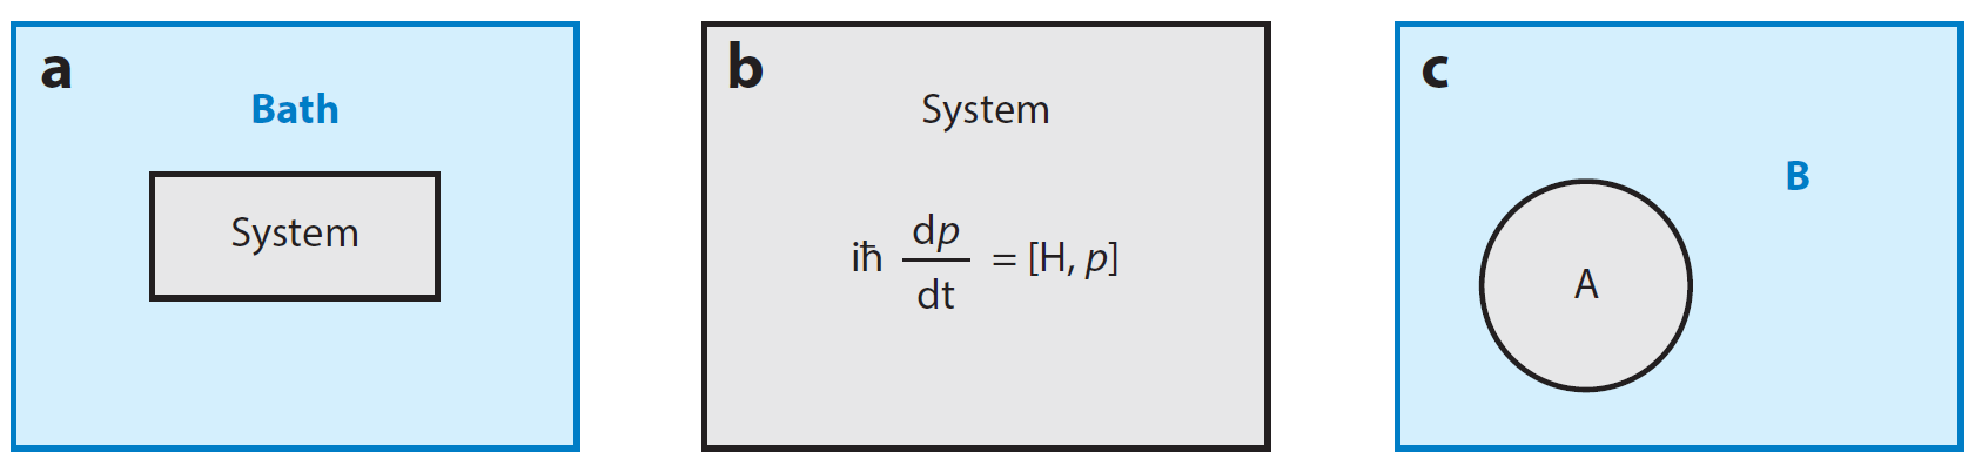
\includegraphics[width=0.8\textwidth]{nandkishore_huse_reservoir.pdf}}
% \caption{Nandkishore, Huse, 2015}
% \end{figure} 
% \begin{itemize}
% \item Thermalization in such systems \textbf{is possible} if subsystem \textbf{B} can act as a reservoir for the subsystem \textbf{A}
% \end{itemize}
% \end{frame}
% \begin{frame}{The eigenstate thermalization hypothesis}

% Thermalization in a system $\Longleftrightarrow$ its \textbf{EIGENSTATES} $\ket{m}$ are \textbf{``THERMAL''}\\\vspace{5mm}
% Eigenstate expectation values equal the ensemble averages at a given temperature:
% $$\bra{m} \hat{O} \ket{m}=\langle \hat{O} \rangle_T$$ \\ \vspace{7mm}
% Not valid for \textbf{INTEGRABLE} and \textbf{MBL} systems

% \end{frame}

% \begin{frame}{Hallmarks of MBL}
% \only<1->{
% \onslide<2->{
% \begin{minipage}{0.3\textwidth}
% \begin{itemize}
% \item \textbf{ABSENCE} of \textbf{ERGODICITY} \vspace{10mm}
% \end{itemize}
% \end{minipage}\hfill
% \begin{minipage}{0.67\textwidth}
% \begin{figure}
% \centering{
% \includegraphics[width=0.67\textwidth]<2->{abanin_thermalization_scheme.pdf}}
% \caption{Abanin, Altman, Bloch, Serbyn, 2018}
% \end{figure}
% \end{minipage}}
% \only<2->{
% \onslide<3->{
% \begin{itemize}
% % \item \textbf{NO} DC conductivity \vspace{7mm}

% \item \textbf{ENTANGLEMENT ENTROPY:}
% 	\begin{itemize}
% 		\item Eigenstates with area-law entanglement
% 		\item Entanglement grows logarithmically in time
% 	\end{itemize}
% % \begin{figure}
% % \centering{
% % \includegraphics[width=0.6\textwidth]<3->{znid_pros_prel_excerpt.pdf}}
% % \end{figure}
% % \end{itemize}}
% % % \only<3->{
% % \onslide<4->{ 
% % \vspace{3mm}
% % \begin{itemize}
% \item \textbf{CHARACTERISTIC ENERGY LEVEL STATISTICS}	
% \begin{itemize}
% 	\item The subject of my current numerical investigations
% 	\end{itemize}
% \end{itemize}}

% \onslide<2->{
% \begin{figure}
% \centering{
% 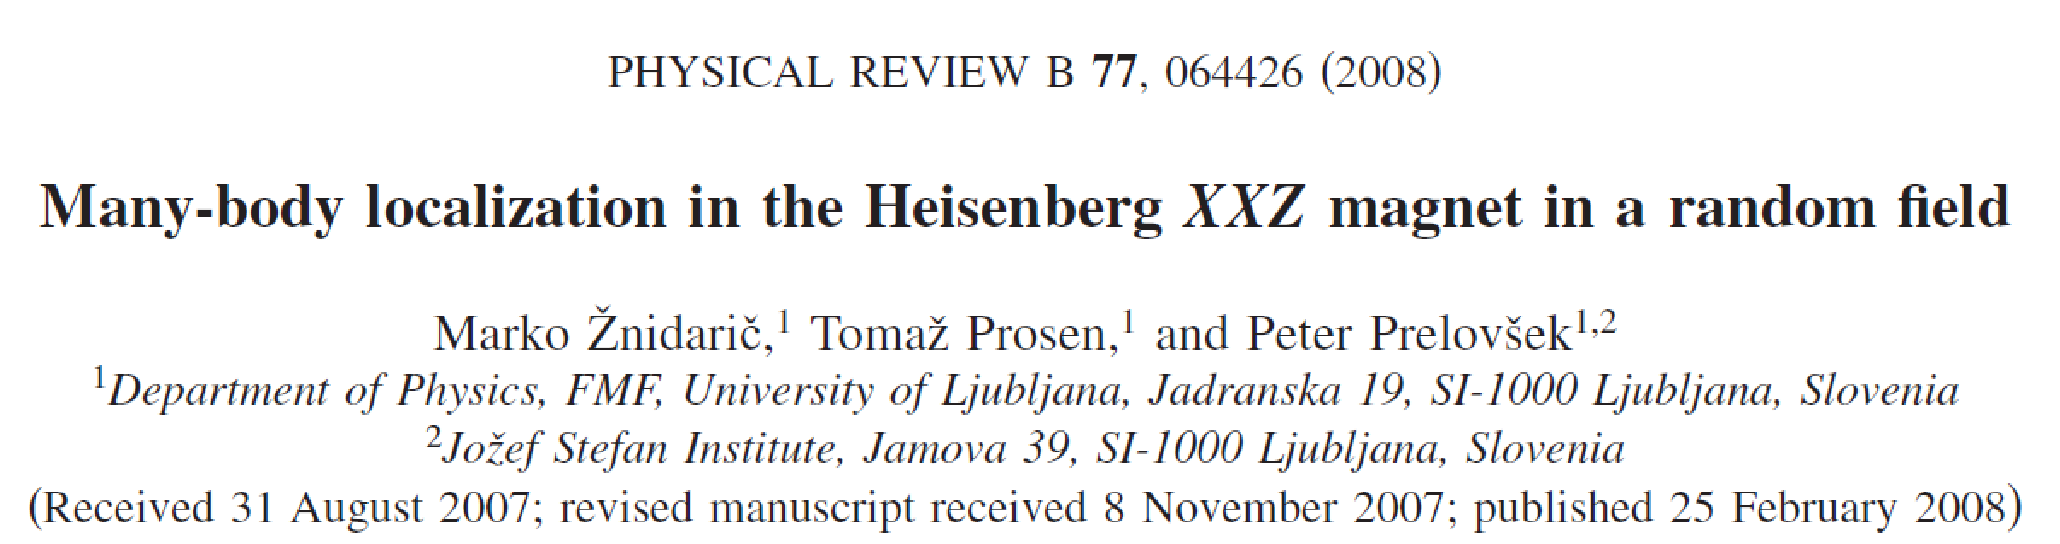
\includegraphics[width=0.6\textwidth]{znid_pros_prel_excerpt.pdf}}
% \end{figure}
% \centering{
% \begin{minipage}{0.4\textwidth}
% \begin{figure}
% \centering{
% 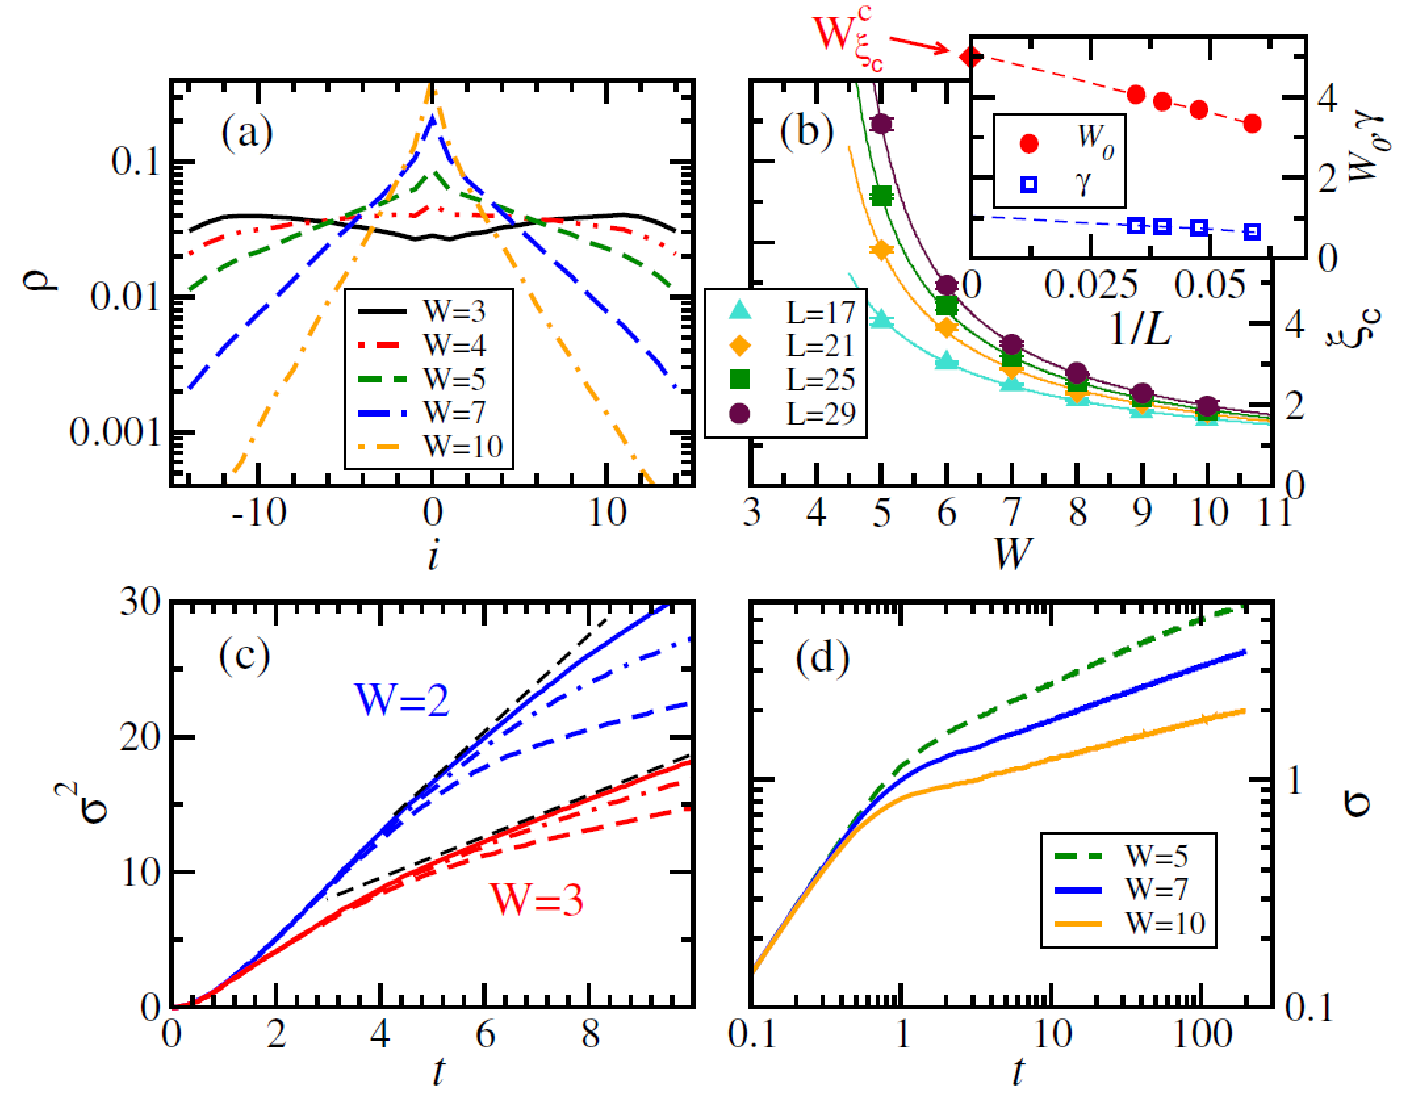
\includegraphics[width=1\textwidth]{gal_bonca_excerpt.pdf}}
% \caption{Lemut, Bonča, Mierzejewski, PRL \textbf{119} (2017)}
% \end{figure}
% \end{minipage}
% \begin{minipage}{0.55\textwidth}
% \centering Absence of ergodicity:
% \begin{figure}
% \centering{
% 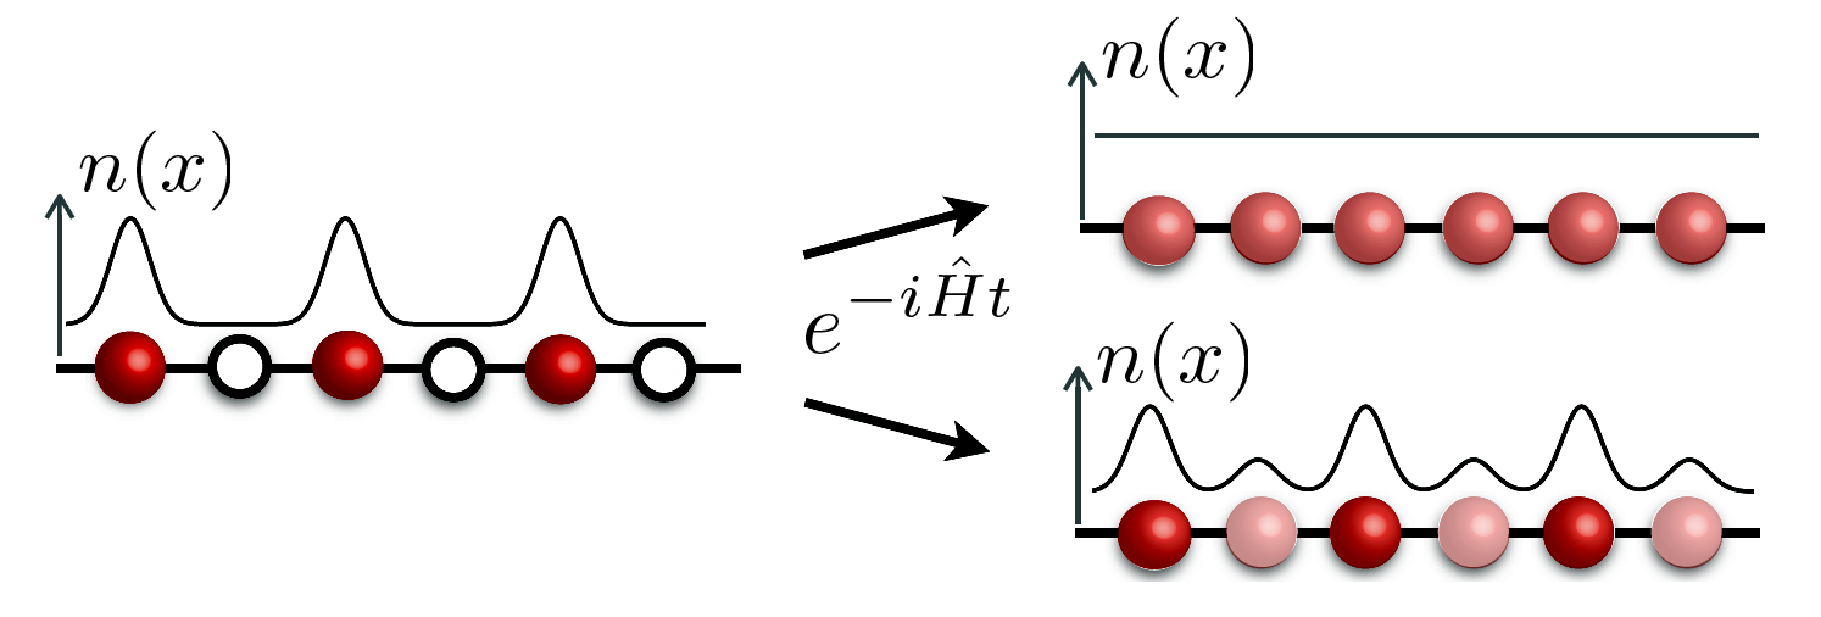
\includegraphics[width=1\textwidth]{abanin_thermalization_scheme.pdf}}
% \caption{Abanin, Altman, Bloch, Serbyn, 2018}
% \end{figure}
% \end{minipage}}
% \begin{minipage}{0.35\textwidth}

% \end{minipage}
% }
% \end{frame}
% \begin{frame}{The tJ model}
% \only<1>{
% \begin{alertblock}{The model Hamiltonian}
% $$H=-t\sum\limits_{i, \sigma} \left(\tilde{c}_{i,\sigma}^\dagger\tilde{c}_{i+1,\sigma} + c.c. \right) + J\sum\limits_i S_iS_{i+1} + \sum\limits_i w_iS_i^z + \sum\limits_{i,\sigma} h_i n_{i,\sigma}$$
% \end{alertblock}
% \begin{itemize}
%  \item The projected fermion operators: $\tilde{c}_{i,\sigma}=(1-n_{i,-\sigma})c_{i,\sigma}$ \vspace{3mm}
%  \item $w_i, h_i$: spin and hole disorder, box distributions with parameters $W$ and $H$ \vspace{3mm}
%  \item We consider the 1D PBC case with $S^z=0$ for a single hole and for finite doping as well
% \end{itemize}}
% \only<2>{
% \textbf{Studies of the hole (sub)diffusion in the tJ model}
% \begin{figure}
% \centering{
% 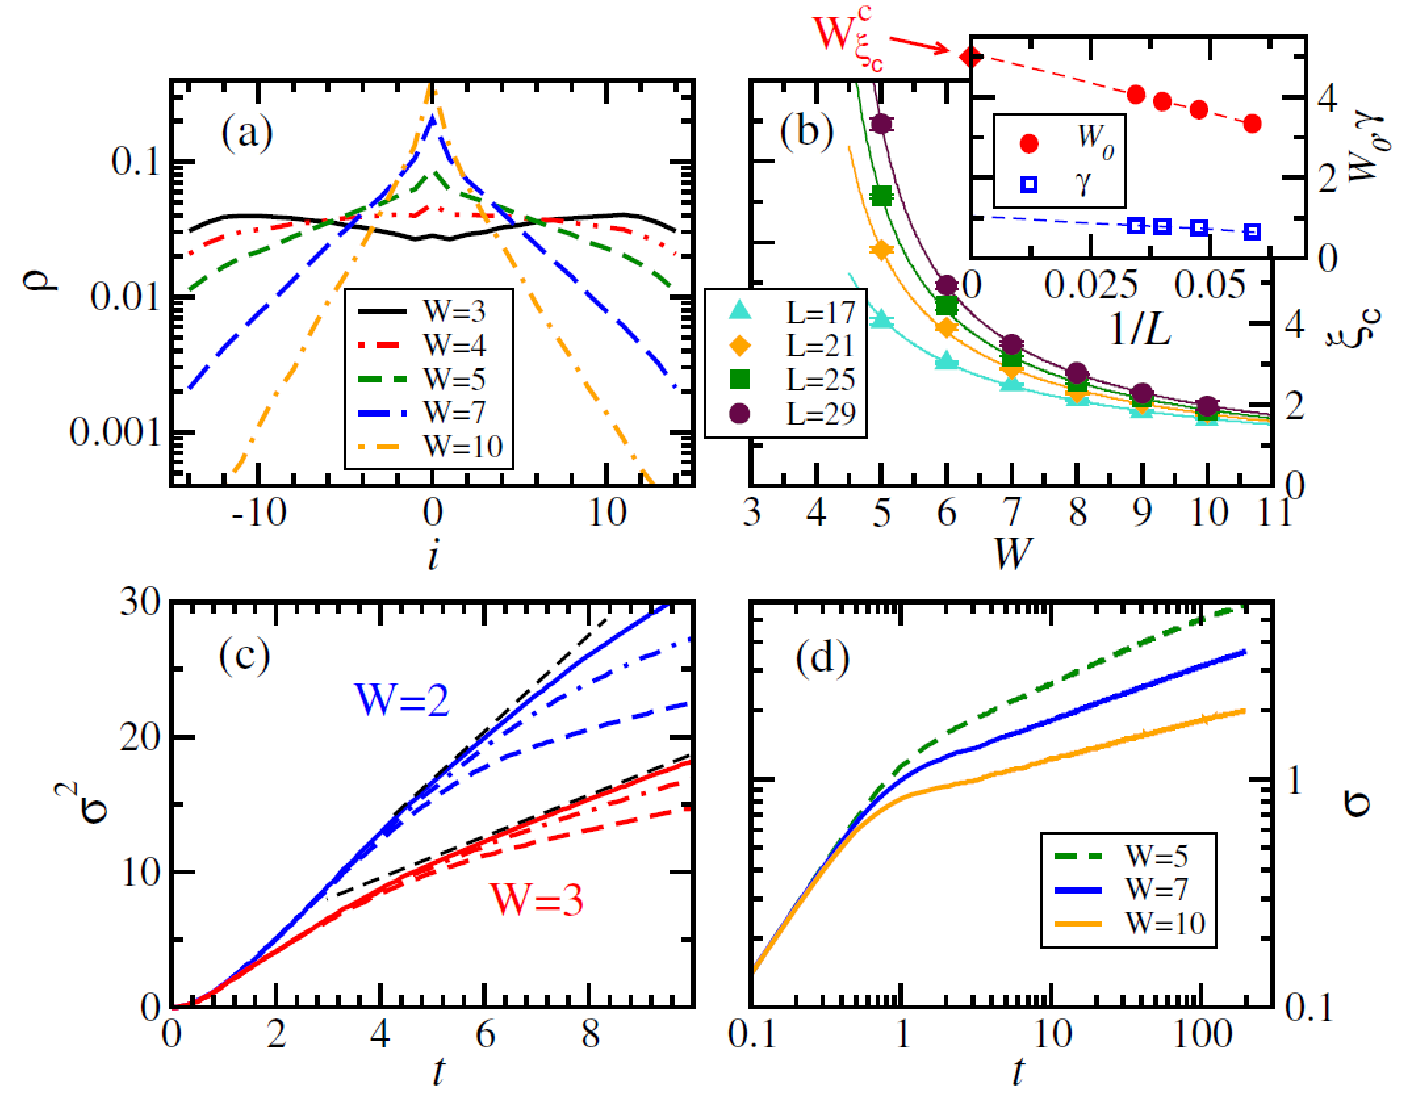
\includegraphics[width=0.65\textwidth]{gal_bonca_excerpt.pdf}}
% \caption{Lemut, Bonča, Mierzejewski, PRL \textbf{119} (2017)}
% \end{figure}


% }

% \end{frame}

% \begin{frame}{Studies of the level statistics}
% \begin{itemize}
% \item We study the \textbf{spectral statistics} of the adjacent energy levels of the tJ Hamiltonian \vspace{7mm}
% \item We lean on the findings of the \textbf{random matrix theory (RMT):} \vspace{3mm}
% 	\begin{itemize}
% 		\item The \textbf{ergodic}/\textbf{quantum chaotic} case: spectral statistics of the Gaussian orthogonal ensemble (\textbf{GOE}) \vspace{3mm}
% 		\item \textbf{MBL} case: no level repulsion, the adjacent energy levels are distributed according to the \textbf{Poisson} distribution
% 	\end{itemize}\vspace{5mm}
% \item Further reading:
% 	\begin{itemize}
% 		\item Oganesyan, Huse, PRB \textbf{75}, 15511 (2007)
% 		\item Y.Y. Atas \emph{et. al.}, PRL \textbf{110}, 084101 (2013)
% 	\end{itemize}
% \end{itemize}

% \end{frame}
% \begin{frame}{Studies of the level statistics}
% \begin{figure}
% \centering{
% 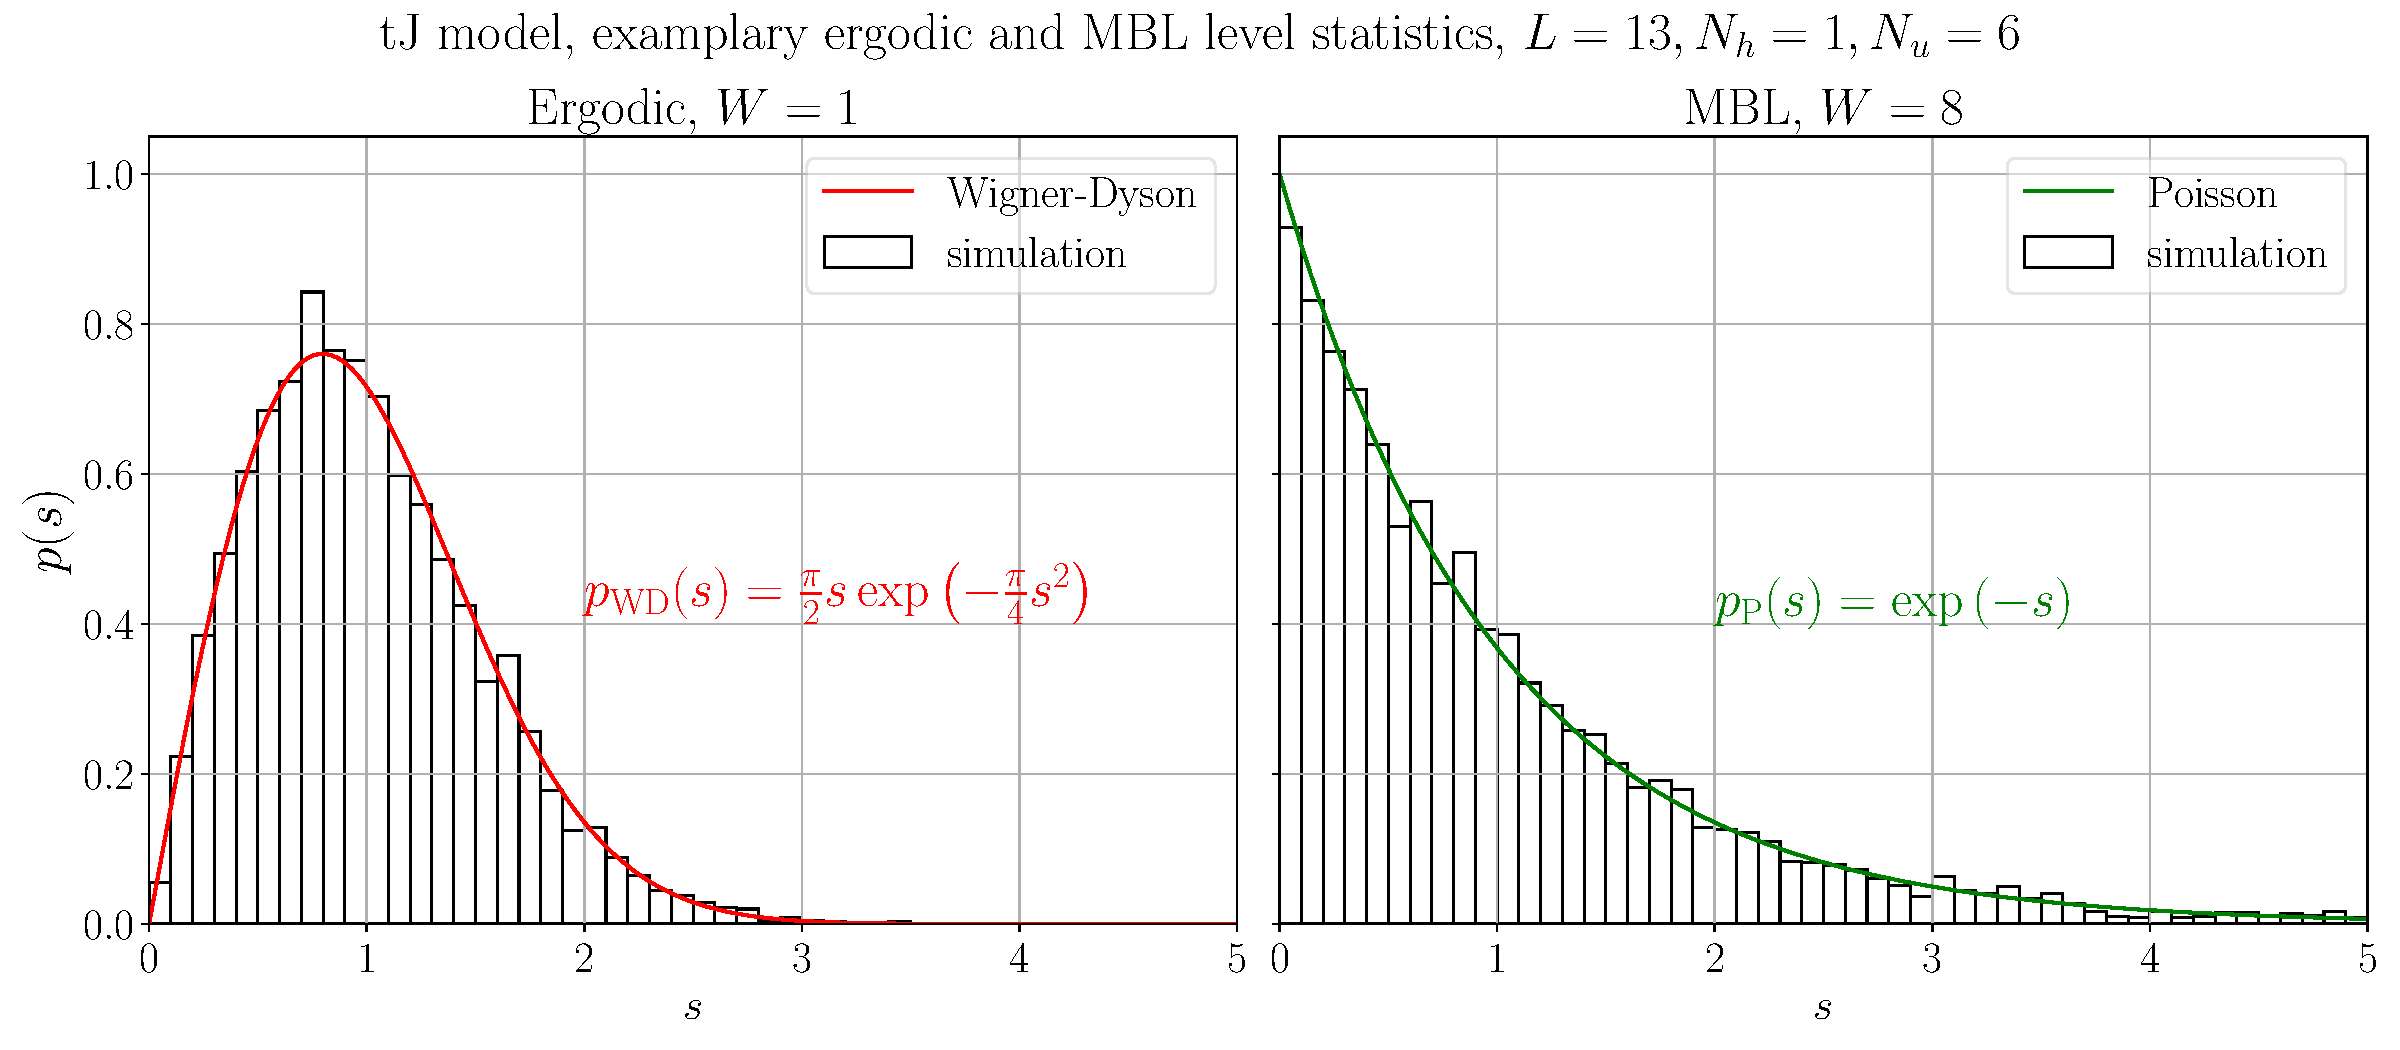
\includegraphics[width=0.9\textwidth]{unfolded_demo_13_1_6.pdf}}
% \caption{$L$ - system size, $N_h$ - number of holes, $N_u$ - number of up spins.}
% \end{figure}
% \begin{minipage}{0.48\textwidth}
% \centering \textbf{GOE:} Wigner-Dyson statistics
% \end{minipage}\hfill
% \begin{minipage}{0.48\textwidth}
% \centering \textbf{MBL:} Poisson statistics 
% \end{minipage}
% \end{frame}
% \begin{frame}{Quantitative analysis}
% \begin{itemize}
% 	\item Gaps between \textbf{adjacent} many body levels:$$\delta_n=E_{n+1}-E_n \geq 0$$
% 	\item We define the \textbf{gap ratio}:\vspace{3mm}
% 	$$0\leq r_n=\min\{\delta_n, \delta_{n-1}\}/\max\{\delta_n, \delta_{n-1}\}\leq 1$$
% 	\item \textbf{GOE} and \textbf{Poisson} average values $\langle r \rangle$ are well known: \vspace{5mm} 
% 	% \begin{itemize}
% 		$$ \langle r \rangle_\mathrm{GOE}=0.5307, \hspace{5mm} \langle r\rangle_\mathrm{P}=2\ln2 - 1 \approx 0.3863 $$
% 		% \item $\langle r \rangle_\mathrm{GOE}=0.5307$ \vspace{3mm}
% 		% \item $\langle r\rangle_\mathrm{P}=2\ln2 - 1 \approx 0.386$
% 	% \end{itemize}
% \end{itemize}
% \end{frame}
% \begin{frame}{Numerical results - single hole case}
% \only<1>{\centering The effect of local symmetry-breaking terms\\ \vspace{4mm}
% \centering  Finite size scaling analysis
% \begin{figure}
% \centering{
% 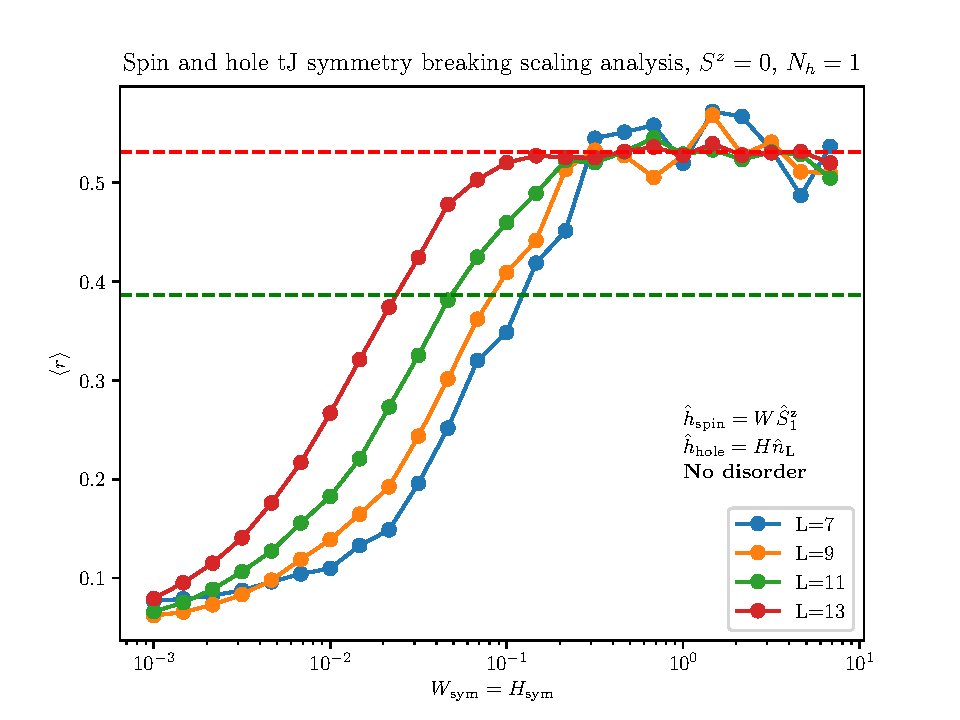
\includegraphics[width=0.7\textwidth]{hole_spin_disorder_sym_break_13_1_6.pdf}}
% % \caption{The effect of weak local symmetry-breaking contributions to the tJ Hamiltonian.}
% \end{figure}}
% \only<2>{\centering Varying spin (left) and hole (right) disorder:
% \begin{figure}
% \centering{
% 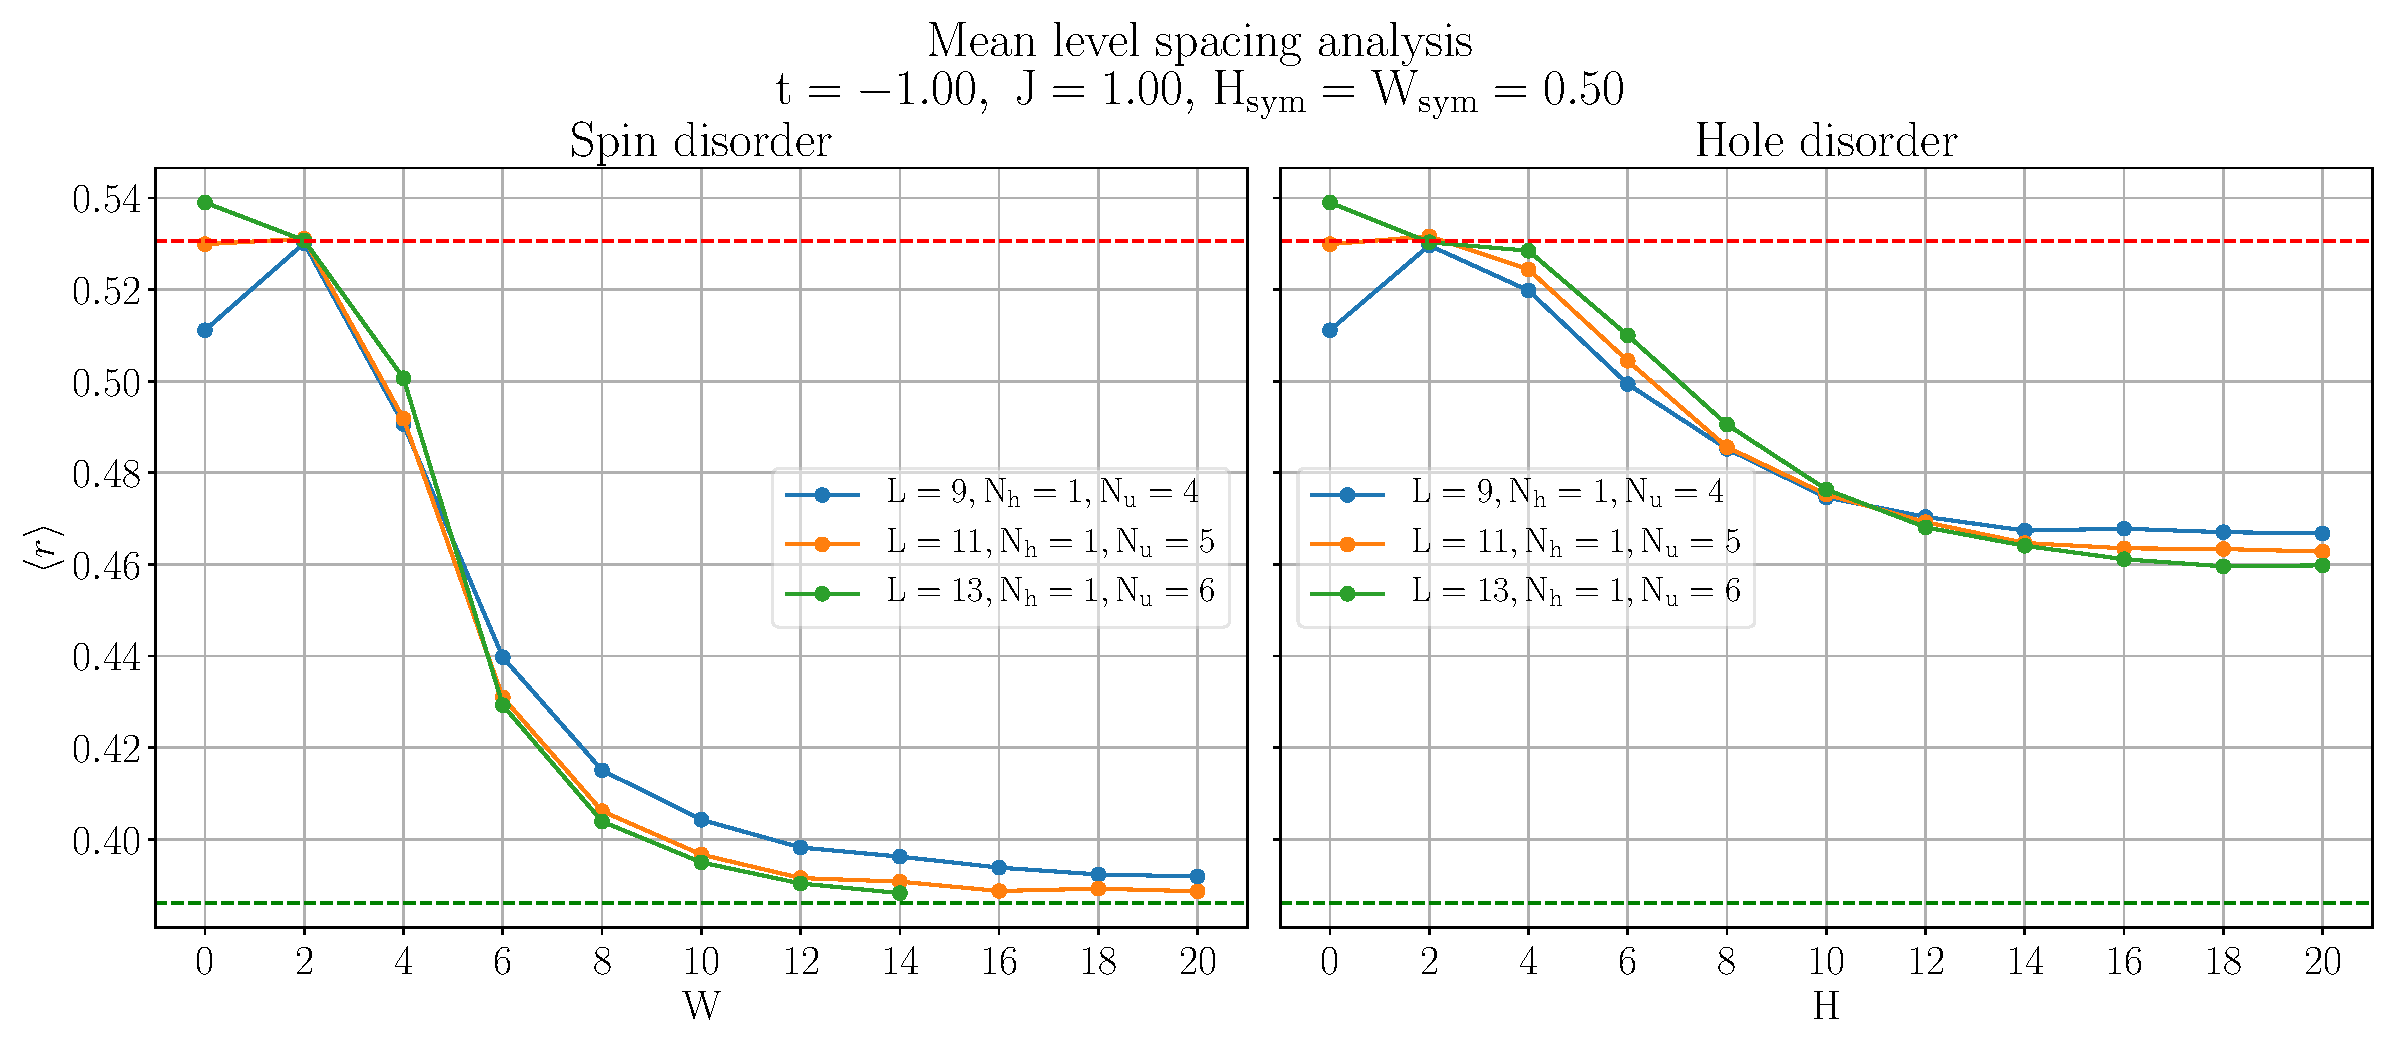
\includegraphics[width=0.9\textwidth]{double_plot_disorder_sym_break_13_1_6.pdf}}
% % \caption{$L$ - system size, $N_h$ - number of holes, $N_u$ - number of up spins.}
% Averaging over different realizations of disorder(s) is performed to obtain final results.
% \end{figure}}
% \only<3>{\centering Finite size scaling analysis\\ \vspace{4mm}
% Hole disorder, no spin disorder.
% \begin{figure}
% \centering{
% 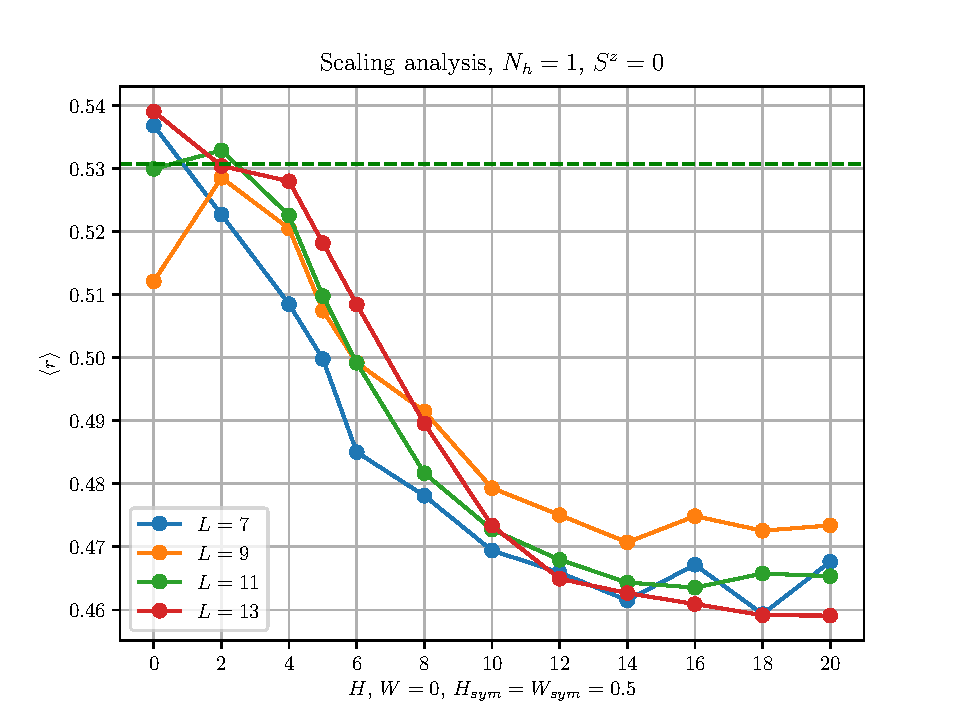
\includegraphics[width=0.68\textwidth]{H_scaling_analysis_sym_break_Nh1.pdf}}
% \end{figure}}
% \end{frame}
% % \begin{frame}{Numerical results - single hole case}
% % % \centering Finite size scaling analysis\\ \vspace{4mm}
% % % \only<1>{
% % % \centering The effect of local symmetry-breaking terms 
% % % \begin{figure}
% % % \centering{
% % % 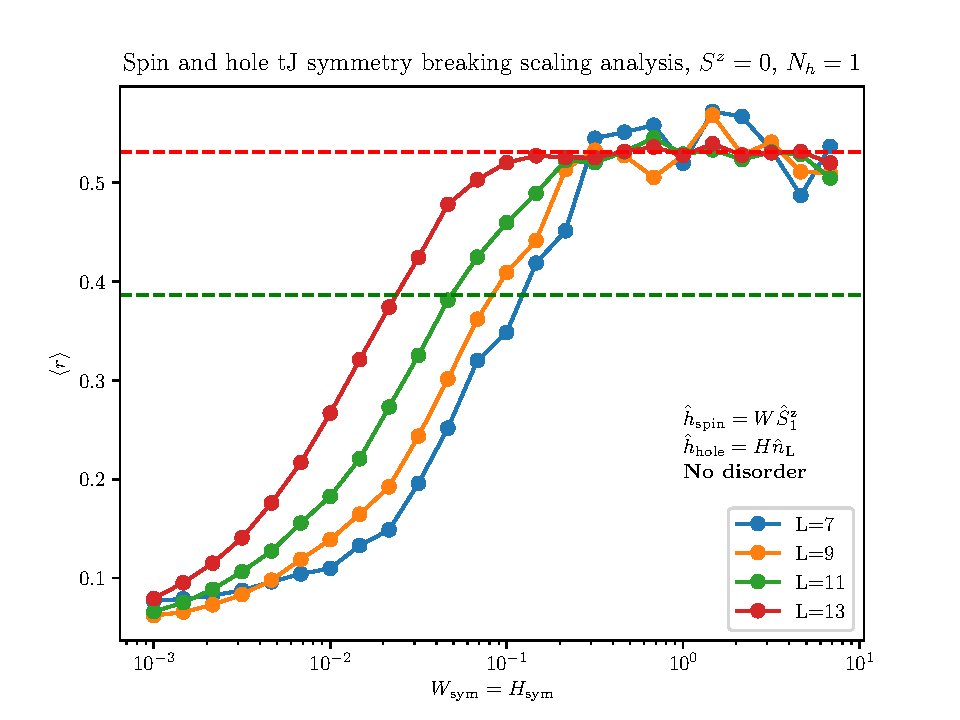
\includegraphics[width=0.7\textwidth]{hole_spin_disorder_sym_break_13_1_6.pdf}}
% % % % \caption{The effect of weak local symmetry-breaking contributions to the tJ Hamiltonian.}
% % % \end{figure}}

% % \end{frame}
% \begin{frame}{Numerical results - finite doping case}
% \centering Varying spin (left) and hole (right) disorder:
% \begin{figure}
% \centering{
% 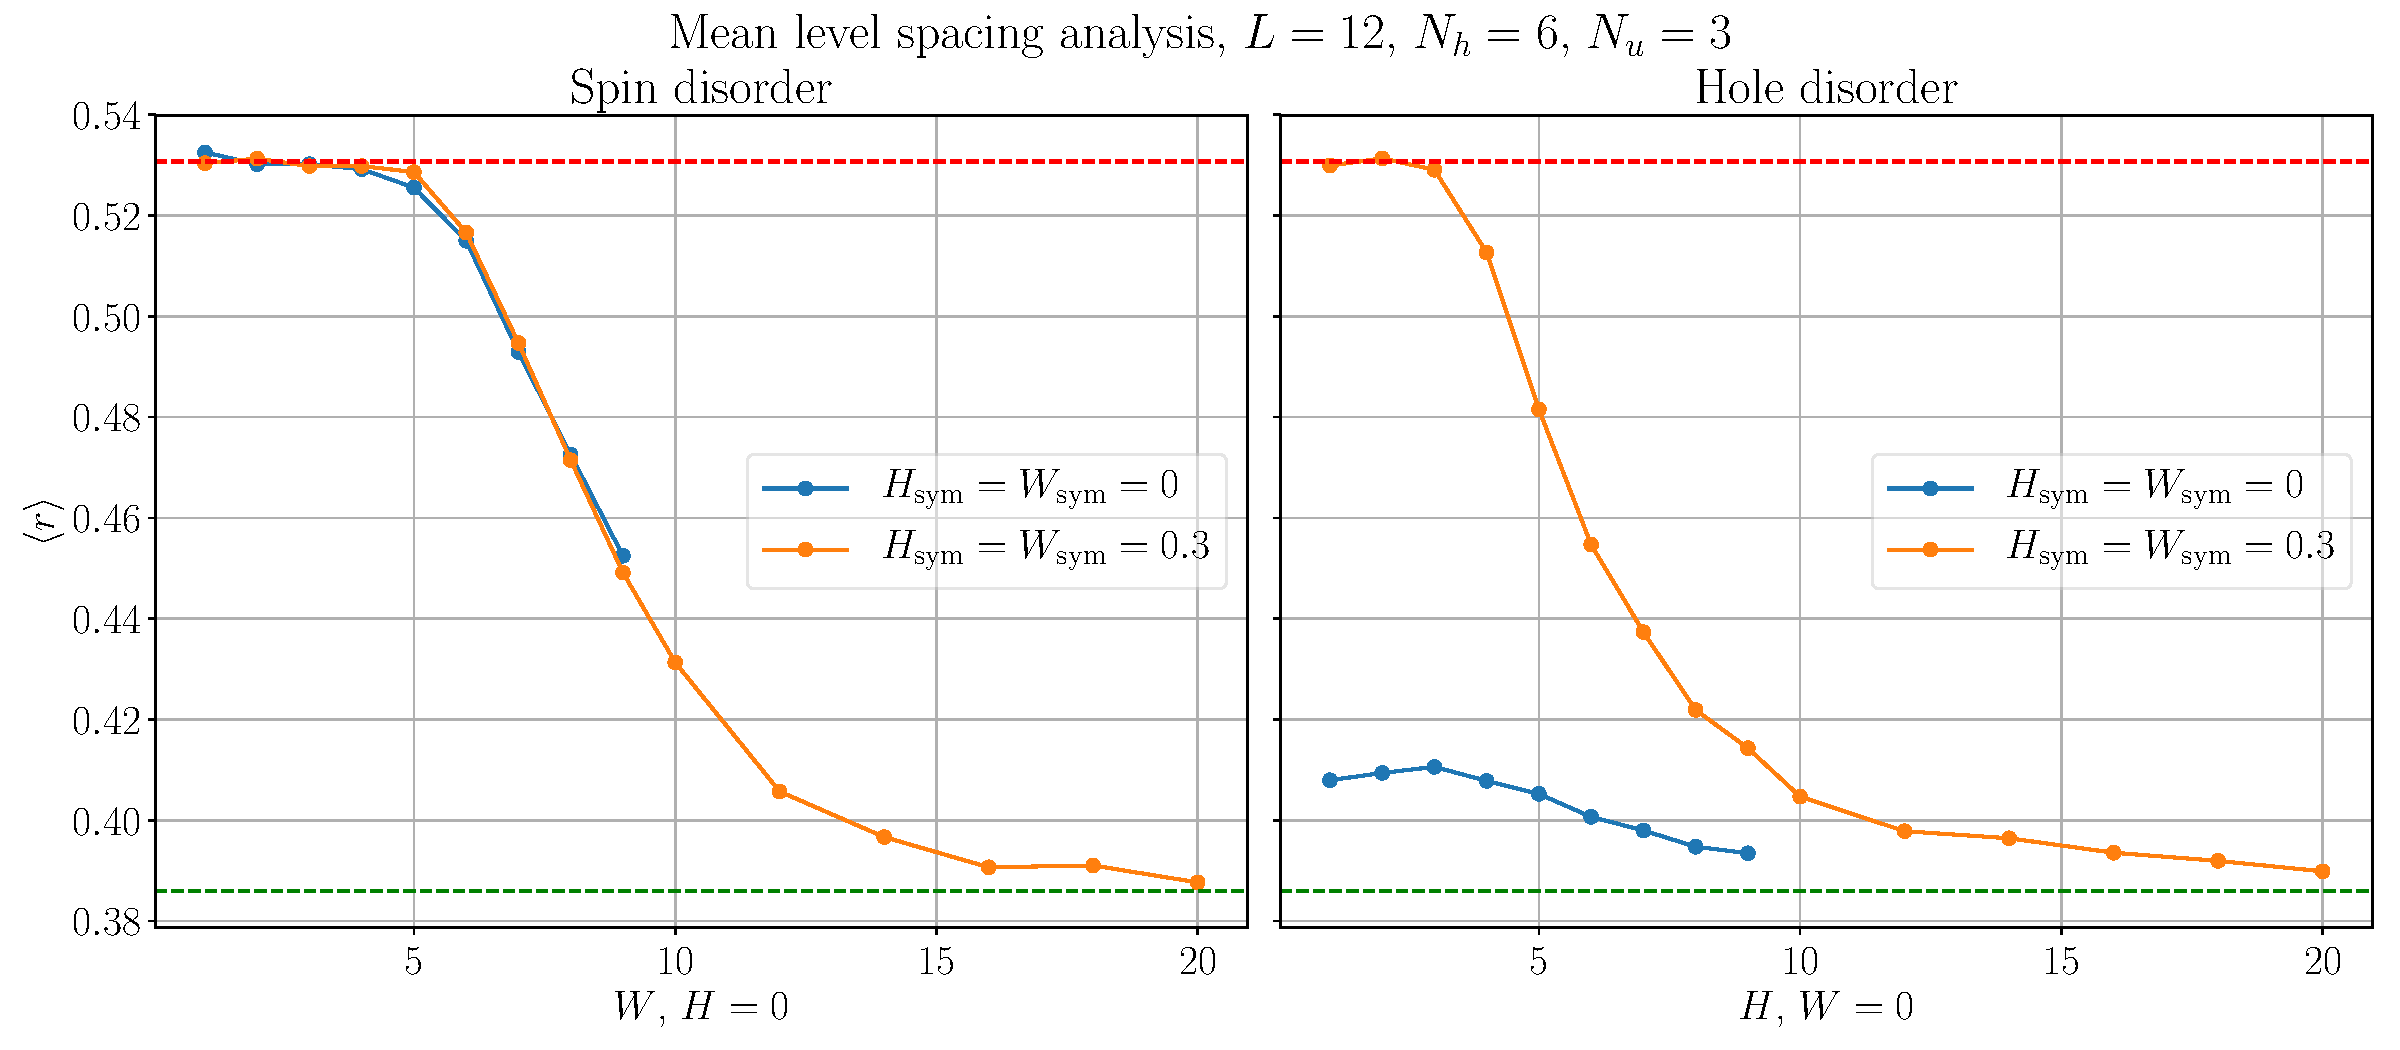
\includegraphics[width=0.9\textwidth]{double_plot_disorder_sym_break_12_6_3.pdf}}
% \end{figure}
% \textbf{Finite hole doping: emergence of MBL for any type of disorder?}
% \end{frame}


% % \begin{figure}
% % \centering{
% % 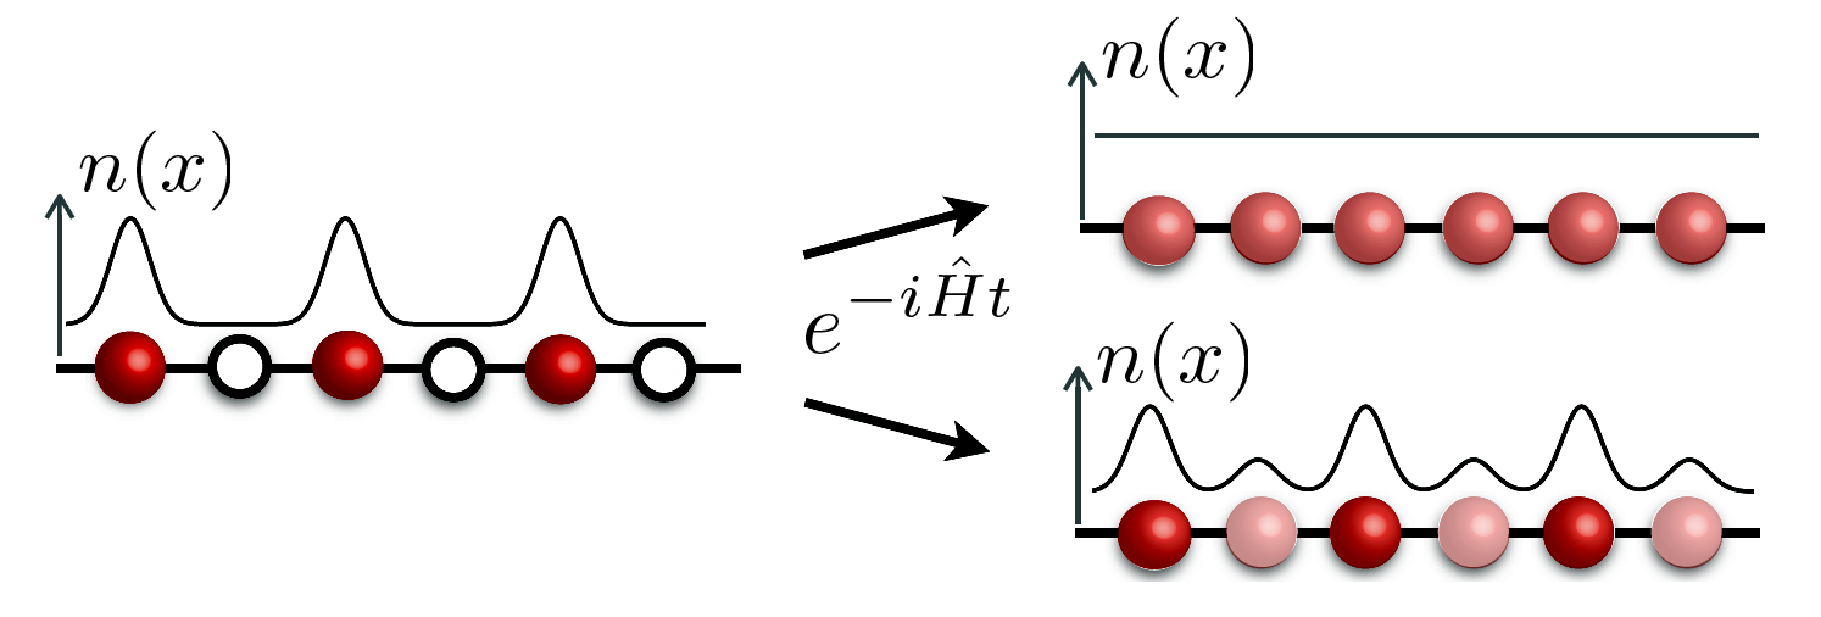
\includegraphics[width=0.8\textwidth]{abanin_thermalization_scheme.pdf}}
% % \caption{Abanin, Altman, Bloch, Serbyn, 2018}
% % \end{figure}
% % \end{frame}
% % \begin{frame}{The eigenstate thermalization hypothesis - ETH}
% % \end{frame}
% \begin{frame}{References and sources of images}
   
%  \begin{thebibliography}{10}
   
%  \beamertemplatebookbibitems
%  % Start with overview books.



   
%  \beamertemplatearticlebibitems
%  % Followed by interesting articles. Keep the list short. 

% \bibitem{Anderson}
% Anderson, P. (1958). \emph{Absence of Diffusion in Certain Random Lattices.} Physical Review, \textbf{109}(5), pp.1492-1505.
% \bibitem{scaling}
% Abrahams E., Anderson P. W., Licciardello, D. and Ramakrishnan, T.V. (1979).\emph{Scaling Theory of Localization: Absence of Quantum Diffusion in Two Dimensions.} Phys. Rev. Lett. \textbf{42}(10), 673
% \bibitem{Kramer}
% Kramer, B. and MacKinnon, A. (1993). \emph{Localization: theory and experiment.} Reports on Progress in Physics, \textbf{56}(12), pp.1469-1564.
% \bibitem{50yearsof}
% Lagendijk, A., Tiggelen, B. and Wiersma, D. (2009). \emph{Fifty years of Anderson localization.} Physics Today, \textbf{62}(8), pp.24-29.



%  \end{thebibliography}
% \end{frame}

\end{document}


